% $Id: phd-thesis-proposal.tex,v 1.5 2008/10/22 12:32:30 rlunsford Exp $
%
\documentclass [11pt] {report}
\makeatletter
\let\orig@xfloat\@xfloat
\makeatother

\usepackage{lscape}		% Allows tables and figures in landscape mode
\usepackage{ohsu-thesis-proposal_3-2012}		% This package is the ohsu thesis style stuff
% \brokenpenalty=100		% uncomment this to see bad word breaks at EOP
% \usepackage{colortab}
\usepackage{epsfig}			% This package allows encapsulated postscript
\usepackage{subfigure}		% This package allows subfigures
\usepackage{graphicx}
\usepackage{footmisc}
\usepackage{amssymb}
%\usepackage[style=acm]{biblatex}
%\renewbibmacro{in:}{%
% \ifentrytype{article}{}{%
% \printtext{\bibstring{in}\intitlepunct}}}
%\addbibresource{nm.bib}

\usepackage{etoolbox}
\makeatletter
\let\@xfloat\orig@xfloat
\patchcmd{\@xfloat}{\columnwidth}{\columnwidth\def\baselinestretch{\@ne}}{}{}
\makeatother

\usepackage{amsfonts}
\usepackage{amsmath}
\usepackage{algorithm}
\usepackage[noend]{algpseudocode}
\usepackage{url}
\usepackage{multirow}
\usepackage{authblk}
\usepackage{rotating}
\usepackage{xr}

% \usepackage{algorithm}
% \usepackage[noend]{algpseudocode}
% \usepackage{url}
% \usepackage{amsfonts}
% \usepackage{amsmath}
% \usepackage{authblk}
% \usepackage{rotating}
% \usepackage{xr}



\renewcommand\floatpagefraction{.9}
\renewcommand\topfraction{.9}
\renewcommand\bottomfraction{.9}
\renewcommand\textfraction{.1} 
\setcounter{totalnumber}{50}
\setcounter{topnumber}{50}
\setcounter{bottomnumber}{50}

\newcommand{\ignore}[1]{}
\newcommand{\rl}[1]{}
\newcommand{\peter}[1]{}
\newcommand{\hints}[1]{}
%\newcommand{\todo}[1]{ **NOW: \emph{#1}**}
%\newcommand{\todolater}[1]{ **LATER: \emph{#1}**}
\newcommand{\todo}[1]{}
\newcommand{\todolater}[1]{}

\makeatletter
\let\latex@xfloat=\@xfloat
\def\@xfloat #1[#2]{%
 \latex@xfloat #1[#2]%
 \def\baselinestretch{1}
 \@normalsize\normalsize
 \normalsize
}
\makeatother

\DeclareMathOperator*{\argmax}{arg\,max}
\newcommand{\degree}{\ensuremath{^\circ}}

%\includeonly{crf}

\begin{document}

% Specify your title here. The "titleline" field should have no line breaks
% in it.
%
\title{Detecting and Analyzing Genomic Structural Variation using Distributed Computing}
\titleline{Detecting and Analyzing Genomic Structural Variation using Distributed Computing}

% Your name (full name, no initials)
%
\author{Christopher Whelan}

% Your previous degree. If you have more than one, use line breaks e.g.,
% \predegrees{degree1 \\ degree2}
%
\prevdegrees{A.B. Computer Science, Harvard University, 1997}
	
	% Heirarchy info
	\discipline{Computer Science \& Engineering}
	\division{Center for Spoken Language Understanding}
	\dept{Institute on Development and Disability}
	\school{School of Medicine}
	\university{Oregon Health \& Science University}

% The following information is for the signature page.
% Note that the definition for principal adviser uses two fields.
% This was needed so that the adviser's name could be placed on the
% abstract page without his title.
%
 %\foursigstrue | \fivesigstrue but don't define BOTH to be true!!
\foursigstrue
\principaladviser{Dr. Kemal S\"onmez}{Associate Professor}
\secondreader{Dr. Brian Roark \\Research Scientist, Google, Inc.}
\firstreader{Dr. Izhak Shafran \\Associate Professor}
\thirdreader{Dr. Lucia Carbone \\Assistant Professor, Dept. of Behavioral Neuroscience}

% This is the expected date that the board of trustee's sign your thesis. They
% meet four times a year and the dates can be obtained from either the Office
% of Admissions and Records (Margaret Day) or from the department secretary.
% In 1991 they were meeting the fourth Monday of each quarter, e.g.,
% January, April, July, October.
\grantdate{June}{2013}

% If you want to copyright your thesis/dissertation remove the line below.
\copyrightfalse		% True by default

% The year of the copyright; usually same as the date the Board of Trustees
% sign the thesis. This won't be printed if \copyrightfalse
\copyrightyear{2013}

% The prefatory section of this style is normally used for the Dedication
% and/or Acknowledgements. You might not want to put this into your thesis
% until the end, to avoid generating it when you are still in the writing
% stage.
%
% The below creates the title page, etc.
\beforepreface

% This is a sample dedication. It should be vertically centered in the page.
% Since the style format doesn't do it for you automatically, you can use
% the following technique.
\ignore{\prefacesection{Dedication}
\vfill
\begin{center}
\end{center}
\vfill
}
% This is a sample acknowledgements page. As in the dedication, it should
% be centered vertically in the page.
%
\ignore{\prefacesection{Acknowledgments}
\vfill
\indent Words.
\vfill
}
% Uncomment the line below if you don't want a list of tables to be printed.
\tablespagefalse

% Uncomment the line below if you don't want a list of figures to be printed.
\figurespagefalse

% \afterpreface generates the table of contents, list of tables (optional),
% and list of figures (optional).
\afterpreface

% Abstract
\abstract{
Genomic structural variations are an important class of genetic variants with a wide variety of functional impacts. The detection of structural variations using high-throughput short-read sequencing data is a difficult problem, with a lack of algorithm implementations that are able to provide the sensitivity and specificity required in research and clinical settings. Meanwhile, the increasing use of high-throughput sequencing is rapidly generating many large data sets, necessitating the development of algorithms that can provide results rapidly and scale to use available cloud and cluster infrastructures. MapReduce and Hadoop are becoming a standard for managing the distributed processing of large data sets, but existing structural variation detection approaches are difficult to translate into the MapReduce framework. I have developed a general framework for structural variation detection in MapReduce, and demonstrated its potential with Cloudbreak, an implementation that detects genomic deletions and insertions with greater accuracy and much faster runtimes than widely-used existing methods. Cloudbreak's formulation of the problem in terms of feature generation makes it amenable to machine learning techniques, which I will demonstrate in a new implementation. In addition to the development of Cloudbreak, I have developed pipelines using existing tools to identify, annotate, and analyze genomic DNA breakpoints within cancer samples and between evolutionarily related species. 
}


% This is where the main body of the thesis starts
%
\body
%\setcounter{chapter}{6}

\chapter{Introduction}\label{chap_introduction}

\todo{comment from Lucia:I really don't like this sentence.
Maybe something along these lines: "Every human cell carries the genetic information needed to accomplish specific biological program. Such information is included in two sets of 23 chromosomes, with each set containing approximately 3 billion DNA bases."

Every normal cell of every human being contains two sets of 23 chromosomes, with the chromosomes in each set holding approximately three billion chained nucleotides of DNA. 

This DNA contains the instructions that the cell uses to code for the proteins that ultimately specify the behavior of the cell, and in aggregate affect the characteristics of the individual to whom the cell belongs. 

The differences between the DNA of the cells in two individuals can explain differences in their physical characteristics, their risk of disease, and their population origin and evolutionary history. 

If one of the cells is cancerous, the differences in the DNA of two cells in one individual can explain the origin of their disease and potentially predict effective treatments.

 through the proteins they code for and the programs of gene expression they regulate}

The aim of the field of \emph{genomics} is to understand the structure and function of the DNA of an organism or population of organisms, with the ultimate goal of understanding how the sequences of nucleotides that make up the genome affect phenotypes and reveal evolutionary history. To do so, it is necessary to identify, characterize, and understand the differences between the DNA from two samples, whether the samples come from two different individuals or two different tissues from the same individual. Given that each sample can contain DNA from multiple cells, and each cell in a human sample contains approximately 3 billion DNA bases packaged into two sets of 23 chromosomes, this is difficult and complex undertaking.

If, as is the case for humans, the species has been widely studied, a \emph{reference genome} is often used in place of one of the samples. This allows variations between individuals to be described as variations between the sample and the reference. Experiments of this type are known as \emph{resequencing} experiments. Assuming that a reference is used, or that the samples come from an individual or individuals from the same or closely related species, the majority of the DNA sequence will be the same between the two samples. In that case, variants can be categorized into one of several forms. The first is a difference of a single base of DNA at a particular location within the genome, or a \emph{single nucleotide variant} (SNV). If the variation is shared between many individuals in a population, these are referred to as \emph{single nucleotide polymorphisms} (SNPs). Another type of variation is the insertion or deletion of a small number of base pairs at a particular location, commonly referred to as \emph{indels}. A final category of variants are genomic \emph{structural variations} (SVs). This term describes variations that affect a large number of bases of DNA (in common usage at least 40 base pairs, ranging up to hundreds of megabases or entire chromosomes). SVs can take a variety of forms: strings of DNA can be deleted, inserted, duplicated, inverted, or translocated to a different chromosome. Because they can be large and frequent, SVs account for the majority of the bases that differ among normal human genomes~\cite{Mills:2011p1611, Conrad:2010ja}.

All of these types of variants can alter the function of a genome in different ways. SNVs can change the sequence of the proteins coded for by genes, sometimes altering their function and sometimes rendering them inactive, or they can alter regulatory elements and cause genes to be expressed at differing levels. Indels typically disrupt the function of a gene or regulatory element. SV's can cause a variety of functional changes, ranging from the deletion of exons to the formation of fusion genes such as the famous Brc-Abl Philadelphia chromosome in chronic myelogenous leukemia~\cite{Kurzrock:2003bz}. 

\todo{change this??}
In fact, SVs are very common in some types of cancer, producing extremely rearranged genomes. Because of this, they have particular importance in cancer research, and it is therefore essential to be able to identify them in biological samples, as well as to characterize their functional impact and the mechanisms of their formation. The SVs that arise in cancer genomes have similarities to those that have arisen between different species in evolution (Figure~\ref{cancer_evolution_breakpoints}). For example, the genomes of gibbon species, while still closely related to humans and other apes, have undergone a variety of chromosomal rearrangements and other structural variations when compared to these other species; many more, in fact, than are typical in species with similar levels of divergence. Understanding the evolutionary changes in gibbons, therefore, may shed light on the much faster processes that take place in progenitor cancer cells.

\begin{figure}
\centering
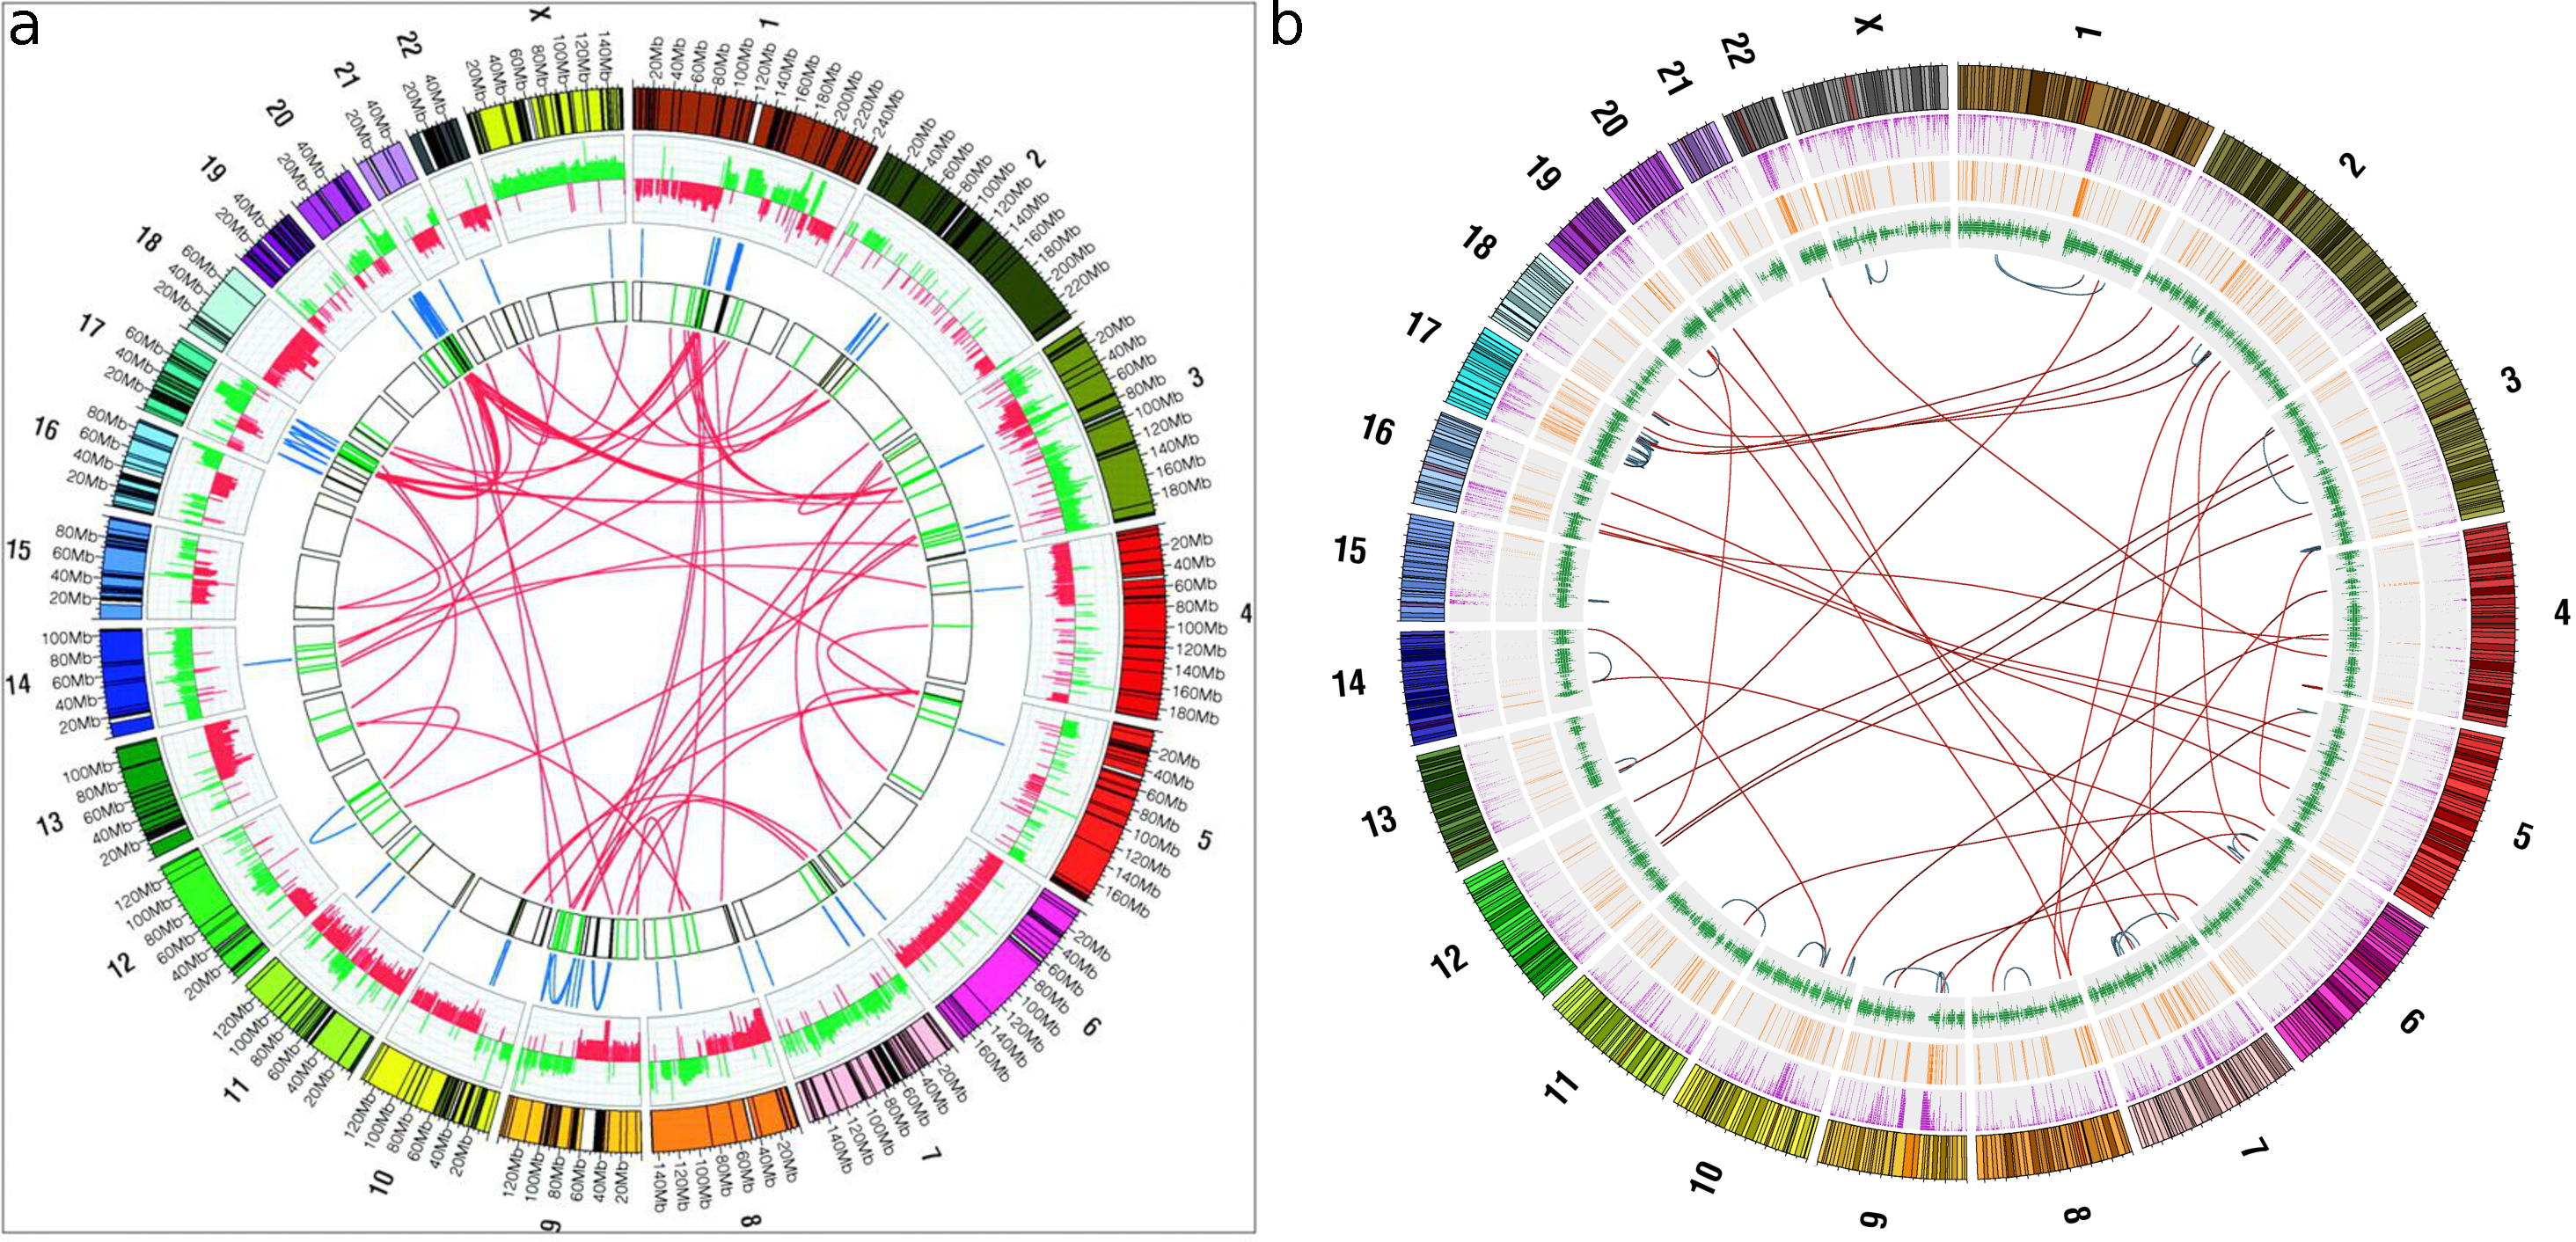
\includegraphics[width=.9\textwidth]{figures/breakpoints_in_cancer_and_evolution.pdf}
\caption{Similarity of genomic breakpoints that occur in cancer and evolution. The regions around the circle represent the human chromosomes. Lines in the centers of the circles show rearrangements between and within chromosomes. A) Somatic rearrangements detected within a breast cancer cell line, adapted from~\cite{Hampton:2009fc}. B) Rearrangements with respect to the human genome sequence present in the gibbon genome, adapted from~\cite{Carbone:2009p1012}.}
\label{cancer_evolution_breakpoints}
\end{figure}

The current technology to detect genomic variations is massively parallel, high-throughput sequencing. This procedure involves amplifying the DNA from a sample and then shearing it into small fragments. The ends of those fragments are then sequenced, producing hundreds of millions or billions of \emph{read pairs} for a sample using current, widely used instruments. The challenge of genomics is then to discover the variants present in the sample using only these short reads. By generating and sequencing enough fragments from a sample (quantified in terms of \emph{coverage}, the average number of reads that cover any one locus in the reference genome), the hope is that it should be possible to capture almost all of the important variants in a given sample. Current practices suggest that 30X average coverage depth is required to achieve accuracy in detecting SNVs. Even with this level of coverage, however, the task is made difficult by errors in the sequencing process, the fact that mammalian genomes are filled with repetitive sequences that make it difficult to ascertain the location in the genome that generated a particular read pair, and the computational challenges of analyzing the volume of data generated.

While SNVs and indels can be characterized relatively well from sequencing data using current algorithmic approaches, the identification of SVs remains challenging. SVs often arise within repetitive regions of the genome, making it difficult to align the reads surrounding them unambiguously to the reference genome. In addition, when the boundaries of an SV (the \emph{breakpoints}) fall within a read sequence, it can be difficult to map that read back to its point of origin in the reference sequence. Although some approaches are based on searching for reads that contain breakpoints, it is often necessary to fall back on other signals present in the read set: the distance between successfully mapped read pairs, which should match the size of the fragments generated in the sequencing protocol, and the depth of reads that cover individual loci along the genome. Detection of SVs with current high-throughput sequencing technology remains a difficult problem, with limited concordance between available algorithms and high false discovery rates~\cite{Mills:2011p1611}.

While current approaches struggle with accuracy, they also often fail to consider speed and scalability. A 30X coverage data set for an individual sample, in compressed format with associated quality scores, is over 100GB of data to analyze. A typical bioinformatic pipeline includes steps to run quality control checks on the raw data; align the reads to the reference genome; perform filtering and recalibration steps after alignment; call SNVs and indels; and finally search for SVs. While a great deal of effort has been put into developing, optimizing, and parallelizing fast methods for alignment and variant calling, SV detection algorithms have not received the same attention, primarily because research in SV detection algorithms has focused on improving accuracy. As large scale sequencing projects like the 1000 Genomes Project and The Cancer Genome Atlas grow, the need for fast and accurate algorithms is becoming more apparent. DNA sequencing is already moving into the clinic, which will only exacerbate this requirement by requiring rapid analysis turnarounds for patients.

One approach to scaling data analysis pipelines is to harness the power of distributed computing using frameworks that tie together clusters of servers. Google's MapReduce~\cite{Dean:2008p277} framework was designed to manage the storage and efficient processing of very large scale data sets across clusters of commodity servers. Hadoop is an open source project of the Apache Foundation which provides an implementation of the MapReduce programming framework as well as a distributed file system (HDFS) for distributing the redundant storage of large data sets across a cluster. Hadoop/MapReduce are rapidly becoming a standard in industrial data mining applications. However, it requires the use of a specific programming model, which can make it difficult to design general-purpose algorithms for arbitrary sequencing analysis problems like SV detection. 

This thesis presents several novel techniques for detecting SVs using distributed computing and machine learning, which derive from the development of an algorithmic framework for SV detection methods in MapReduce. In particular, the main contributions are:

\begin{itemize}
 \item The description of an algorithmic framework for solving SV detection problems in Hadoop and MapReduce based on the computation of local features along the genome from paired end mappings (Chapter~\ref{chap_framework}).
 \item The development in this framework of a software package, Cloudbreak, for discovering genomic deletions up to 25,000bp long, and short insertions, which improves accuracy over existing approaches and uses distributed computing to achieve dramatically faster runtimes (Chapter~\ref{chap_cloudbreak_impl} and Chapter~\ref{chap_cloudbreak_eval}).
 \item An evaluation of the strengths and weaknesses of Cloudbreak when tested on several real and simulated data sets (Chapter~\ref{chap_cloudbreak_eval}).
 \item An exploration of the use of local features as described in Chapter~\ref{chap_framework} to reformulate SV detection as a sequence labeling problem, and the corresponding implementation and evaluation of a conditional random field model to create a novel method for integrating different signals of structural variations (Chapter~\ref{chap_crf}).
\end{itemize}

In separate work not related to the algorithmic developments listed above, we also present the results of data analysis projects which examined the SVs that have massively rearranged the genome of the gibbon in an evolutionary time frame. This has led to the additional contribution of:

\begin{itemize}
 \item Identification of sets of genomic features that are enriched near the breakpoints of the structural variations are present between gibbons and humans. These include segmental duplications and some families of transposable elements, as well as evolutionarily shared transcription factor binding sites. This analysis enhances our understanding of gibbon genome rearrangements. (Chapter~\ref{chap_breakpoint_analysis}).
\end{itemize}

A preliminary version of parts of this work was peer-reviewed and accepted for oral presentation at the Third Annual RECOMB Satellite Workshop On Massively Parallel Sequencing (RECOMB-seq). A preliminary breakpoint analysis was published in~\cite{Capozzi:2012bb}. Throughout this document, I have tried to explicitly identify any work that was carried out by my collaborators.


\chapter{Biological Background}\label{chap_background}

In this chapter we will explore the nature of structural variations, discuss the mechanisms that may be behind their formation, and their effect on phenotypes and disease. We will then describe high-throughput sequencing and discuss the typical informatics pipelines that researchers create to analyze sequencing data, placing SV detection within the context of the other types of computation that must be done to support end-to-end analysis. Finally, we will discus the challenges that the increasing number and size of sequencing data sets represent.

\section{Structural Variations}

As we described in the introduction, structural variations (SVs) are rearrangements, relative to some reference genome sequence, of sequences of DNA with a length longer than 40 or 50bp. These can take the form of deletions of reference sequence, insertions of novel sequence, duplications of sequence, inversions of orientation of a stretch of sequence with respect to the rest of its chromosome, or translocations of sequence from one chromosome to another. Deletions, insertions, and duplications are also frequently referred to as \emph{copy number variations} (CNVs). In addition, many complex SVs exist in which these simple SV types are combined.

SVs can occur and become part of a gene pool on several different biological and time scales. On the smallest level, SVs can rearrange the genomes of individual cells within an organism. If the SV contributes to the cell's ability to proliferate, or occurs in conjunction with another mutation that does so, it can give rise to a tumor, or a new subpopulation or clone within an existing tumor. On a population scale, the genomes of individuals within a species harbor SVs with respect to one another, either because they were transmitted through the germline or because they arose \emph{de novo} in certain individuals. Finally, on a larger scale, SVs within a species may become fixed, contributing to differences between the genomes of varying species on an evolutionary scale.

\subsection{SV Effects on Phenotype and Disease}

On all of these levels, SVs are associated with differences in phenotypes and have been shown to associate with many types of disease, making them an important area of study. Knowledge of these effects has of course been shaped by the types and number of SVs that technology and collected data has allowed us to detect, and is therefore biased towards larger variants that were discoverable before the advent of modern array and sequencing technologies. 
Cancer genomes contain many SVs that have been linked to cancer progression. The famous Brc-Abl mutation~\cite{Kurzrock:2003bz} mentioned previously is the most famous example of a fusion gene, in which portions of the genome coding for two different genes are made adjacent due to an SV. This results in the creation of new gene which can take on novel functions, which in turn drive cancer growth. Fusion genes can be caused through any type of SV that causes a novel adjacency between regions of the genome, including deletions, duplications, translocations, and inversions, and there have been dozens of recurring fusion genes identified across varying cancers to this point~\cite{Annala:2013ks}. In another example, the genomic locus that contains the MYC gene, which among other functions regulates cell proliferation~\cite{Eilers:2008jk}, is frequently duplicated multiple times in breast cancer cells~\cite{Escot:1986tn}. These duplications change the amount of protein made by the cell, causing a dosage-related defect in cell regulation. In other cancer cells, a dramatic process called \emph{chromothripsis} has been observed, in which entire chromosomes appear to ``shatter'' and then be pieced back together. This gives rise to hundreds of SVs, some of which can promote cancer development~\cite{Stephens:2011bm}. On the other end of the spectrum in terms of variant size, small deletions of less than 150bp in untranslated coding regions of genes have been observed to contribute to aberrant gene expression in leukemia~\cite{Hosokawa:1998wi}.

On the scale of the human population, SVs and CNVs have been implicated in a variety of diseases (for a comprehensive recent review see Weischenfeldt et al.~\cite{Weischenfeldt:2013fm}). The best studied of these are large CNVs, including deletions or duplications of genes. These can can include variants that arise \emph{de novo} in individuals, either giving rise to rare disorders~\cite{Lupski:1998ip} or contributing to the risk of more common conditions such as Crohn's disease~\cite{McCarroll:2008jt}, autism~\cite{Sebat:2007bs}, and schizophrenia~\cite{Walsh:2008kp}. However, most CNVs in the human genome are polymorphic within the population and contribute to human genetic diversity~\cite{McCarroll:2008p265}. The rise of microarrays and high-throughput sequencing has sped the discovery of smaller variants that affect coding sequence by deleting exons. To give one recent example, an 8kb deletion of an exon in the BAG3 gene has been tied to risk for cardiomyopathy~\cite{Norton:2011ev}. \todo{etc.}

There are also numerous examples of deletions that affect human phenotypes even though they do not directly overlap with the coding regions of genes, instead interacting with regulatory elements that control gene expression levels. For example, deletions ranging from 36kb to 319kb in size that are over one megabase away from the SOX9 gene locus can alter its expression by removing an enhancer element, giving rise to a rare cleft palate syndrome called Pierre Robin sequence~\cite{Benko:2009dq}. Expanding on this idea, a survey of CNVs between inbred mouse strains showed that 28\% of gene expression differences between strains could be statistically explained by CNVs, but that only 7\% of the identified CNVs directly overlapped one of the differentially expressed genes, suggesting that SVs may shape many aspects of organism phenotypes in complex ways~\cite{Cahan:2009ef}. In another dramatic example from other species, the well-studied stickleback fish, which has repeatedly evolved adaptations to fresh water in several locations around the world as it moved from the sea into lakes, owes one of those adaptations, the loss of spines on its pelvis, to recurrent sub-2kb deletions of an enhancer that regulates the Pitx1 gene~\cite{Chan:2010hz}.

\todo{This last case points to the value that can be gained by studying SVs that have been shaped by, or helped to shape, evolutionary processes. Hahn gene duplications.. Ventura segmental duplications in gorilla.. Gibbon karyotype.. }

\subsection{Mechanisms and Signatures of SV Formation}\label{section_sv_mechanisms}

Given that many of the phenotypic effects of SVs described above are deleterious to the organism, it is natural to ask how they arise in genomes. Biologists have identified several different mechanisms that can cause SVs. By studying many of the genomic disorders mentioned in the previous section, geneticists found that often CNVs recur in different individuals at the same locations in the genome. Examining these locations revealed that they are homologous to genomic sequence repeated elsewhere in the genome in the form of segmental duplications, stretches of DNA that are over 1kb in length with greater than 90\% sequence identity\cite{Sharp:2006fy}. This helped to identify the process of non-allelic homologous recombination (NAHR)~\cite{Liu:2012if}. In the best studied form of NAHR, the cell attempts to repair DNA in the cell that has suffered double-stranded breaks (DSBs). To do so, it attempts to find homologous DNA in the nucleus that can be used as a template to repair the broken strand. However, repeats in the genome provide the opportunity for DNA from the wrong genomic location to be used in this repair process, creating genomic breakpoints in the repaired DNA. In mammals, as little as 295bp of non-allelic homologous sequence can be responsible for NAHR events~\cite{Liskay:1987wt}. The human genome contains many copies of transposable elements, including 500,000 of the LINE family and over one million of the \emph{Alu} family, with average lengths of 6kb and 300bp, respectively. Both \emph{Alu}~\cite{Lehrman:1985tn} and LINE~\cite{Robberecht:2013kw} are frequently involved in NAHR events. As these and other transposons copy themselves into new locations in the genome, they also give rise to their own class of SV, mobile element insertions (MEIs), which leave their own signatures of small tandem site duplications (TSDs) at either end of the insertions.

In contrast to NAHR, other mechanisms can create SVs without extensive sequence similarity at the breakpoint. Non-homologous end joining (NHEJ) and microhomology mediated end joining (MMEJ) are two such processes~\cite{Hastings:2009fv}. Both of these mechanisms involve the repair of DSBs in the cell and typically result in SV breakpoints that have very small (less than 20bp) homologies on either side. Other processes of SV formation that leave a signature of microhomologies at the breakpoint are Fork Stalling and Template Switching (FoSTeS)~\cite{Lee:2007fy} and microhomology-mediated break-induced replication (MMBIR)~\cite{Hastings:2009fv}. In these models, as the cell replicates all of its DNA two replication forks can switch DNA templates, causing complex structural variations to form. Finally, the chromothripsis process mentioned above also gives rise to microhomologies~\cite{Liu:2011p1751}.

Given that different SV formation mechanisms have different signatures that can be determined by the presence of varying amounts of duplication or homology at or near the breakpoints, it is possible to analyze SVs to gain insight into their formation in different contexts. For example, Conrad et al.~\cite{Conrad:2010if} surveyed CNVs from 40 unrelated individuals using a targeted sequencing method that enabled them to determine exact sequences around the breakpoints of some events. They found that although the best studied human genomic disorders are due to recurrent SVs caused by NAHR, NHEJ and MMEJ were responsible for the great majority of CNVs they were able to detect, a result later confirmed by the 1000 Genomes Project~\cite{Mills:2011p1611}, although studies in mice have found that MEI may be more frequent albeit harder to detect~\cite{Yalcin:2011tm}. \todo{cancer?} In Chapter~\ref{chap_breakpoint_analysis}, we will discuss efforts to analyze the sequence context of genomic rearrangements between species.

\section{High-Throughput Short-Read Sequencing}\label{section_sequencing}

The pace of analysis of genome rearrangements and SVs has risen dramatically with the widespread adoption of high-throughput short-read sequencing (for a review see Shendure and Ji~\cite{Shendure:2008jh}). In early projects to interrogate SVs in DNA samples researchers had to painstakingly map individual variants using time-consuming microscopy (for very large rearrangements), fluorescence in situ hybridization (FISH), southern blotting, or polymerase chain reaction (PCR) assays~\cite{Aten:2008dh}. The development of microarray technology allowed simultaneous testing of many genomic probes on a sample, although the probes had to be developed using prior knowledge of what variants to expect. Short-read sequencing, however, allows direct DNA sequence data to be collected in a relatively unbiased way from the entire genome, overcoming these limitations.

High-throughput short-read sequencing technology is currently dominated by Illumina, Inc. (San Diego, CA), and unless otherwise noted we will be referring to data generated by Illumina instruments when we refer to short-read or next-generation sequencing data in this document. The Illumina sequencing process begins with creation of genomic DNA library, which has billions of small fragments of DNA, sheared randomly across the genome, with adapter sequences attached to the ends. These adapters attach randomly to locations on the surface of the sequencing instrument's \emph{flow cell}, and then are amplified in place to form clusters on the flow cell, each consisting of thousands of copies of a DNA fragment from the library. The sequencer then initiates a process in which the complements of each strand of DNA in the clusters are synthesized one base at a time. Each complementary base added to the new molecule contains a fluorescent tag, and the instrument takes a picture of the flow cell at each step. Pooling the color signal from each strand in a cluster, the sequencer optically analyzes the image from each time step to call the base at that position in each cluster. Because all clusters can be analyzed simultaneously in a single flow cell image, Illumina's sequencing instruments can now process billions of fragments at the same time. Illumina's HiSeq 2500 instrument, the current throughput leader, can produce 1.2 billion paired-end reads, or 120Gb of data, in 27 hours. 

While this technique produces unprecedented amounts of sequencing data, the downside is that read lengths are limited by the extent to which the synthesis process can be regulated and kept in sync across all of the clusters on the flow cell. In Illumina's current high-throughput instruments, this limits read lengths to 100bp or 150bp. This can be mitigated somewhat through techniques that sequence both ends of a DNA fragments, producing the paired-end reads referred to earlier. If the size of the fragment is approximately, the distance between the two sequenced ends can be estimated, as we will discuss in detail in Section~\ref{section_read_pair}. These paired-end techniques typically use fragments of between 250 and 500bp, although in some cases \emph{mate pair} fragment sequencing can produce reads from the ends of much larger fragments (6-8kb).

Because nearly half of the human genome is made up of repetitive elements, the analysis of the short reads produced by these sequencing technologies present a unique set of challenges~\cite{Treangen:2011p1810}. As we mentioned earlier, repetitive elements such as \emph{Alu} and LINE appear many times in the genome. If a read, or pair of reads, falls entirely within a single repetitive element, it will be impossible to determine the location in the genome it came from if there has not been enough sequence divergence of the repeat over evolutionary time to distinguish it from the others. Because many SV formation mechanisms depend on sequence homologies at the breakpoints, they are particularly likely to fall into repeats in the genome, complicating the task of SV detection from short-read data.

In addition to making SV detection difficult, short-read sequencing -- by the unprecedented volume of data it produces -- also presents challenges to developing scalable infrastructure and algorithms for processing sequencing data in general. We will return to the problem of SV detection in the next chapter, and in the remainder of this chapter will give an overview of the applications of high-throughput sequencing data, and will discuss the computational challenges they represent.

\subsection{Sequencing Analysis Pipelines}\label{section_pipelines}

To transform raw sequencing reads into usable information typically requires a series of discrete steps. As genomic bioinformatics has matured, these have been increasingly modularized and made into components that can be connected together to create analytics pipelines designed for particular applications. In this section, we will describe pipelines for several of the most popular applications of high-throughput sequencing.

\subsubsection{DNA Resequencing}

As we mentioned in Chapter~\ref{chap_introduction}, resequencing projects attempt to identify variants present in the genomic DNA of samples from a population for which there exists a reference sequence. Variants can then be described in standard formats (typically VCF, the Variant Call Format~\cite{Danecek:2011gz}) that describes them in terms of the sequence and coordinates of the reference. These can then be used in study designs such as case control or genome wide association studies, or, in clinical contexts, can be searched directly using prior knowledge for variants likely to be associated with diseases or conditions.

\begin{figure}
\centering
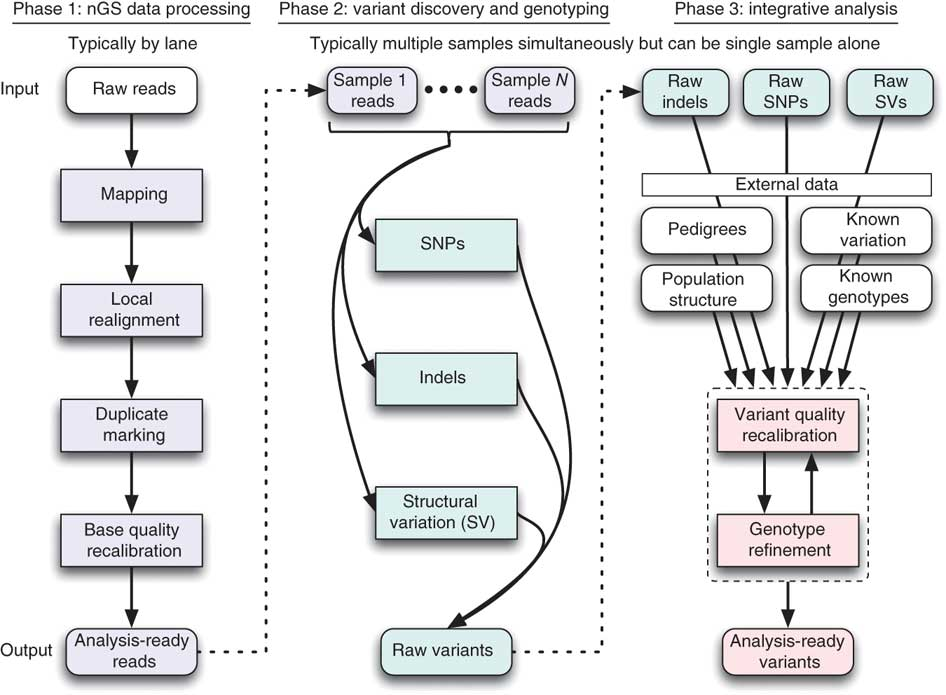
\includegraphics[width=1\textwidth]{figures/ng-806-F1.jpg}
\caption{A full computational pipeline for high-throughput short-read DNA resequencing projects. This figure describes the Genome Analysis Toolkit (GATK) best practices pipeline, and is representative of the computational steps involved in a full resequencing pipeline designed to process many samples simultaneously. Reprinted by permission from Macmillan Publishers Ltd: Nature Genetics 43:5pp491-498~\cite{DePristo:2011fo}, copyright 2011}
\label{gatk_pipeline}
\end{figure}

Figure~\ref{gatk_pipeline} shows a high-level representation of the steps involved in a large-scale resequencing project using the Genome Analysis Toolkit~\cite{DePristo:2011fo}. The main components are:

\begin{enumerate}
\item \textbf{Quality Control and Data Preparation.} Although not shown in Figure~\ref{gatk_pipeline}, most pipelines typically begin by running a set of reports to assess the quality of the raw data, often with a standardized QC suite such as FastQC~\cite{fastqc} and data preparation steps including trimming the portions of the input sequences that have base calls with low confidence scores or that contain sequence that matches known artifacts of the sequencing process (adapter trimming). These components operate on raw data in the FASTQ format~\cite{Cock:2010ky}.

\item \textbf{Read Mapping.} In this phase, reads are mapped to the reference genome to find their most likely coordinates of origin. There exist a wide variety of short-read mappers that are heavily optimized for the task of aligning short DNA sequences to reference genomes (for a survey from several years ago see Li and Homer~\cite{Li:2010p10}). These typically use some form of a seed-and-extend strategy, in which exact matches of portions of the input read to the reference genome are found quickly using pre-computed indices. These indices can take the form of hash tables or some form of enhanced suffix array, or more popularly, the suffix trie equivalent FM-index~\cite{Ferragina:2000vl}, which uses the Burrows-Wheeler Transform (BWT)~\cite{Lossless94ablock-sorting} to convert a suffix trie into a highly compressed structure that is particularly useful for indexing highly repetitive genome sequences while still giving fast (under most conditions linear in the length of the query pattern) lookup times. These exact matches are then extended using direct comparisons or through dynamic programming techniques such as the Smith-Waterman alignment algorithm~\cite{Smith:1981up}. Examples of hash-based aligners include Novoalign~\cite{novoalign} and MOSAIK~\cite{2013arXiv1309.1149L}, while BWA~\cite{Li:2009p836} and Bowtie 2~\cite{Langmead:2012jh} are popular BWT-based aligners. The output of this step is typically in the Sequence Alignment/Map (SAM) format~\cite{Li:2009vz}, which in addition to the reads stores their alignment coordinates on the reference genome, mapping quality scores, and information about mismatches to the reference.

\item \textbf{Local Realignment, Duplicate Marking, and Recalibration.} In some pipelines there is often an additional quality control step after read mapping. PCR amplification in the preparation of sequencing libraries from DNA samples can give rise to duplicate fragments, which are typically identified and removed at this point. In addition, this step can include a more expensive realignment phase for groups of reads that appear to span short insertions and deletions (INDELs, typically under 40bp in size), and a recalibration of the base call quality scores reported by the sequencer based on the empirically observed distribution of mismatches between the reads and the reference sequence~\cite{DePristo:2011fo}.

\item \textbf{Variant Calling.} The next phase includes calling of single nucleotide variants (SNVs), INDELs, and SVs. To call SNVs and indels, algorithms examine each possible variant indicated by mismatches of reads to the reference. They typically evaluate the number of reads supporting the variant against the total number of reads at that location, as well as prior beliefs, in Bayesian framework. Popular SNP and INDEL callers include the GATK~\cite{McKenna:2010p1051}, SAMtools~\cite{Li:2009vz}, and SOAPsnp~\cite{Li:2009p1236}. In some cases, multiple samples from a population are examined simultaneously, giving additional power to detect variants in that population. We will discuss SV callers in more detail in Chapter~\ref{chap_related_work}.

\item \textbf{Integrative Analysis/Filtering.} After raw variants have been called, additional sources of outside information can be used to adjust their confidence scores or filter out false positives. This can include data from existing catalogs of genomic variants or knowledge about the population structure of the samples. If multiple samples from the same pedigree are being sequenced, data can be reconciled based on the principles of inheritance. DePristo et al.~\cite{DePristo:2011fo} describe one such set of filters appropriate for a large scale study involving many individuals from a population. In Section~\ref{section_aml_pipeline} we will describe a simple filtering scheme we implemented for a cancer sequencing project.

\end{enumerate}

\subsubsection{Other Sequencing Applications}

In addition to DNA resequencing to detect genomic variants, there are many other applications of short-read sequencing. We will not go into detail on how each works, but will briefly list the goals and major informatic components of several of the most common so that we can address a full picture of the computational scaling challenges that short-read sequencing represents. 

\begin{itemize}
\item \textbf{RNA-seq.} In RNA-seq (see Oshlack et al.~\cite{Oshlack:2010kr} for a review), the goal is to interrogate the expression of genes across samples, for example in different disease conditions. Rather than sequencing DNA, libraries are constructed from RNA taken from the sample. Similarly to DNA resequencing, the reads are QC'd and aligned to the reference genome, although there are read mappers especially designed for RNA-seq that include functionality to map reads over exon junctions. The reads that map to annotated genes on the reference are then analyzed and quantified to determine  the genes that are being expressed in the sample, along with their relative expression levels and isoforms.

\item \textbf{ChIP-seq} The intent of ChIP-seq (reviewed by Park~\cite{Park:2009gl}) is to determine the locations in which DNA, or the chromatin that contains it, is being bound by protein transcription factors or modified, with the ultimate goal of determining the modifications that are driving gene expression. In this case fragments of DNA that are bound to the protein of interest are preferentially separated and sequenced. After read trimming and mapping, the locations of binding events can be identified by searching for ``peaks'' of coverage on the reference genome.

\item \textbf{\emph{de novo} Assembly} When there is no reference genome present for the organism being sequenced, the goal is to try to reconstruct the full sequence of the input genome based only on the short reads. A full discussion of \emph{de novo} assembly algorithms is beyond the scope of this section; for a review see Nagarajan and Pop~\cite{Nagarajan:2013cq}. The general approach is to build a graph representing overlaps between the reads in the form of either a string graph~\cite{Myers:2005iq} or a \emph{de Bruijn} graph, and then walk the graph to determine the underlying sequence. This is complicated by the fact that mammalian genomes are highly repetitive. The need to construct a graph data structure linking all of the input reads means that assembly is typically an extremely memory-intensive process, making it difficult to distribute computation.

\end{itemize}

There are of course additional sequencing applications, including workflows specifically designed for cancer-related projects and metagenomics, which aims to discover all of the microorganisms present in a diverse sample. 

\subsection{Big Data from Sequencing}

All of these sequencing applications are creating an enormous amount of data that is pushing the limits of the computational infrastructure and algorithms used by biologists. For example, the European Bioinformatics Institute currently stores multiple petabytes of genomic data, and that amount has been taking less than one year to double since the advent of high-throughput sequencing in 2008~\cite{Marx:2013dz}. This has led to increasing calls for new bioinformatics strategies for storing, managing, sharing, and processing that data. An early recognition of the fact that computational requirements would soon outstrip the capacity of the prevailing model of processing data on local servers in individual laboratories created a movement towards centralized databases and processing on remote servers enabled by standardized data formats and annotations~\cite{Stein:2008gh}. After the creation of large scale cloud compute services, bioinformatics leaders quickly realized their potential to ease the burden of processing sequencing data~\cite{Stein:2010gp,Schatz:2010js,Schadt:2010dp}. In particular, they noted that cloud computing would allow the scaling of compute infrastructure to meet demand, rather than having to plan compute clusters capable of handling the predicted peak load. In addition, cloud computing offers a potential solution to the problem of sharing large data sets in the highly collaborative field of genomics; by storing large data sets in the cloud that are accessible to multiple groups, collaborators could become less dependent on the prevalent strategy of sharing data by shipping hard drives to one another. Several of these arguments also noted that cloud computing is a natural fit for creating distributed algorithms that can be scaled to larger data sets by adding more compute resources, in particular through the use of the MapReduce programming model~\cite{Schatz:2010js,Schadt:2010dp}. We will return to the topic of cloud computing in Chapter~\ref{chap_framework}, where we will develop a framework for detecting SVs in MapReduce. Before we do so, however, we will review existing algorithms for SV detection in Chapter~\ref{chap_related_work}.


\chapter{Algorithms for Structural Variation Detection}\label{chap_related_work}

In Chapter~\ref{chap_background}, we described the biological impact of SVs, and the development of short-read sequencing technology, along with the computational challenges they represent. In this chapter we review existing algorithms for SV detection based on short-read sequencing data, with an emphasis on the amount of data they integrate into their analysis and their ability to be parallelized or scaled. We will review the four major computational strategies for SV detection and examine several exemplar approaches in depth. Finally, as a demonstration of how SV detection can fit into the pipeline models we described in Chapter~\ref{chap_background}, we will describe a small pipeline for SV detection that we developed that used an existing tool, BreakDancer, to characterize SVs in a low-coverage cancer sample. 

\section{The Four Signals of SVs in Sequencing Data}

Most popular SV detection algorithms can be placed into one of four categories based on the type of signal it extracts and analyzed from sequencing data sets~\cite{Alkan:2011p547,Koboldt:2012gj}. The first three categories depend upon first aligning short reads to the reference genome. In Section~\ref{section_sequencing}, we described paired-end sequencing, in which both ends of a single DNA fragments are sequnced. Read pair (RP) based methods use the distance between and orientation of the mappings of these sequenced ends to identify the signatures of SVs. RP approaches are the most commonly used based on their ability to detect many types of SVs and their computational tractability~\cite{Alkan:2011p547}. Read depth (RD) approaches identify regions of the genome with anomalous coverage by read mappings, which may indicate the presence of copy number variations (CNVs). Split Read (SR) approaches attempt to find local mappings of portions of individual reads that span SV breakpoints. Finally, assembly-based methods attempt to construct as much of the genome sequence as possible directly from the reads, without first mapping them to the reference genome. The constructed sequence is then compared to the reference to identify SVs. Beyond these four categories, several recent approaches have attempted to integrate more than one type of signal to increase accuracy. In this review of published alogorithms, we will focus on those that are built to handle whole-genome DNA resequencing from a single sample at a time; there are of course other approaches for different applications, including SV detection from targeted resquencing data such as exome sequencing, and approaches which are designed only to operate on many samples at once.

\section{Read Pair Approaches}\label{section_read_pair}

Given correct mappings of paired reads to the reference genome and a reliable estimate of the length of the fragments from which the reads came, it is relatively straightforward to detect SVs. For example, Figure~\ref{rp_signatures} shows the signatures of insertions and deletions based on the insert size of paired-end mappings: deletions lead to a longer distance between read mappings than expected, insertions to a shorter distance. Similarly, because protocols determine the orientation in which the read will be sequenced, inversions can be detected if they diverge from expectations. Finally, inversions can be detected if the reads map to different chromosomes in the reference genome. These ideas were first applied to high-throughput short-read sequencing data by Korbel et al.~\cite{Korbel:2007p544} and Campbell et al.\cite{Campbell:2008p539}, who built upon strategies developed for analyzing SVs through the mapping of sequenced ends of larger DNA fragments (bacterial artifical chromosomes (BACs) and fosmids) from non-high-throughput sequencing data~\cite{Volik:2003fh,Raphael:2003ug,Tuzun:2005bp}.

\begin{figure}
\centering
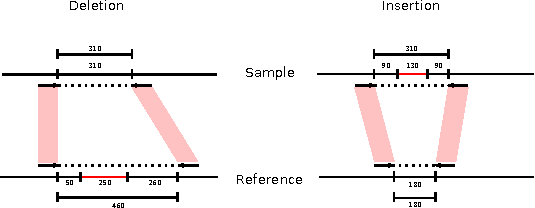
\includegraphics[width=\textwidth]{figures/rp_signatures.pdf}
\caption{Detecting deletions and insertions from the distance between mappings of paired reads. For the case of a deletion, a fragment with a 310bp internal insert size is created from the sample DNA, in a region in which 250bp has been deleted relative to the reference. The two reads when mapped to the reference will be 460bp apart, providing evidence for a deletion if we expect the internal insert size to be approximately 300bp. A 310bp internal insert size fragment that overlaps a 150bp insertion in the sample, conversely, will give a distance between reads of 180bp when mapped to the reference.}
\label{rp_signatures}
\end{figure}

Most read pair approaches use a basic strategy outlined in Figure~\ref{rp_method_workflow}. They begin by separating paired end mappings onto the reference genome into those that are \emph{concordant} and those that are \emph{discordant}, i.e. those which deviate from the expected insert size or orientation of the library. With only a few exceptions, discussed below, RP approaches discard concordant pairs and consider only discordant pairs for the remainder of their analysis. The next step is then to cluster the discordant mappings such that each cluster coherently supports a single candidate SV call. Finally, they filter or rank the candidate SV calls, for example only keeping those with support from multiple discordantly mapped read pairs. 

The BreakDancerMax component of BreakDancer~\cite{Chen:2009p3} is probably the most widely used of these algorithms\footnote{Based on a sampling of Google Scholar citation counts as of 12/28/2013: BreakDancer, 270; VariationHunter, 153; PEMer, 111; GASV, 65; SVDetect, 46.}. As described above, BreakDancer first searches for discordant read pairs based on a hard threshold on the distance between mapped paired reads. It then looks for regions of the genome that anchor more discordant read pairs than expected according to its model; if two of these regions are connected by a minimum number of discordant read pairs, it calls an SV that links them. It calls breakpoints based on the inner boundaries of the two connected regions, as illustrated in Figure~\ref{rp_method_workflow} (d), and then assigns a confidence score by computing the likelihood of the SV based on a null model in which discordant read pairs are distributed across the genome according to a mixture Poisson model.

Other RP-based tools include GASV~\cite{Sindi:2009gu}, PEMer~\cite{Korbel:2009dy}, and SVDetect~\cite{Zeitouni:2010p8} (adds additional filters). These all operate on similar principles, differing primarily in the method used to cluster discordant read pairs that support the same potential SV call. 

Read pair approaches have the advantage of being theoretically able to detect any type of SV except for multiple copy number duplications. Their disadvantages stem from the fact that they depend on comparing mapping distances between reads to the unknown size of the fragments from which they came. This means that they cannot capture the breakpoints of SVs with single nucleotide resolution, and that they depend on having a sequencing library with a tight distribution of fragment sizes in order to have power. In addition, the fact that many SV breakpoints occur in regions with high sequence similarity to other parts of the genome, as discussed in Section~\ref{section_sv_mechanisms}, means that it may be difficult to unambigously map reads to those locations.

\begin{figure}
\centering
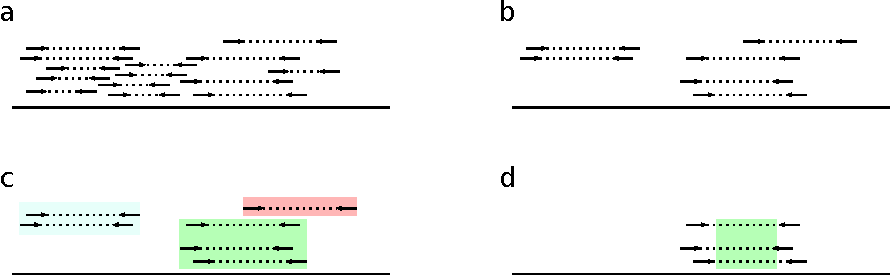
\includegraphics[width=\textwidth]{figures/rp_method_workflow.pdf}
\caption{The general algorithmic steps of a classic read-pair algorithm. a) The algorithm accepts a set of alignments of paired reads to the reference as input. b) The algorithm identifies discordant read pairs. c) Discordant pairs are clustered to find groups that could support the same algorithm. d) Clusters of discordant read pairs are filtered (in this case, by the number of supporting read pairs), and bounds on the potential breakpoints are identified.}
\label{rp_method_workflow}
\end{figure}

\subsection{Ambiguously Mapped Read Pairs}

Many of these approaches use only reads that are unambiguously mapped to the reference genome; this has the advantage of using the same set of alignments that are used for calling SNVs and indels in most sequencing pipelines. A second group of RP methods attempt to include discordant read pairs which cannot be unambiguously mapped to the reference genome in their analysis, in an effort to improve sensitivity in repetitive regions of the genome. One approach to incorporating this type of information can be found in \emph{soft clustering} algorithms, which assign each ambiguously mapped read pair to one of its mappings such that it clusters with other discordant read pairs. These approaches include VariationHunter~\cite{Hormozdiari:2009p284}, which allocates ambiguously mapped reads by optimizing to a maximum parsimony explanation of all discordant reads; HYDRA~\cite{Quinlan:2010gf}, which takes a similar approach based on heuristics, and GASVPro~\cite{Sindi:2012kk}, which uses a Markov-Chain Monte Carlo sampling strategy to assign a read to its correct mapping. Even so, however, most methods use only a limited number of ambiguous discordant mappings per read pair, in part because of the storage and computational requirements necessary to process all or most ambiguous mappings of each read pair in a high-coverage data set.

\subsection{Concordant Read Pairs}\label{section_mixture_of_distributions}

ChopSticks (homozygous deletions only, refine sv calls with concordant pairs)~\cite{Yasuda:2012ij}

Finally, CLEVER~\cite{Marschall:2012ek} took an alternative approach and showed that rather than classifying pairs as concordant or discordant and considering only those that are discordant, considering the distribution of all insert sizes allows the detection of smaller events. 

Another class of hybrid solution explicitly models the expected number of concordant and discordant pairs at normal and variant locations, effectively combining RP and RD strategies. MoDIL~\cite{Lee:2009da} and the BreakDancerMini component of BreakDancer~\cite{Chen:2009p3} model the distribution of insert sizes at candidate locations in the genome using a Gaussian mixture model. This has two advantages: because reads are not categorized as concordant or discordant based on a hard threshold, it is possible to detect smaller insertions and deletions; and these approaches can explicitly model the zygosity (presence of the variant on one or both of the pairs of chromosomes in the cell) of the variant in the sample, and potentially classify the variant as homozygous or heterozygous. The disadvantage of this approach in these implementations has been the computational requirements, although as we shall see in Chapter~\ref{chap_cloudbreak_impl}, this strategy can be effectively parallelized if approached in the right way.

\section{Read Depth Approaches}

Read-depth (RD) approaches consider the changing depth of coverage of concordantly mapped reads along the genome to infer the presence of SVs. For example, a homozygously deleted region will have zero coverage in the reference genome, while a region that has been duplicated many times, as can happen in some regions of the genome and in some cancers, will have a much higher coverage than average. These approaches differ mainly in the statistical and signal processing techniques used to identify anomalous regions. For example, CNVnator~\cite{Abyzov:2011bk} uses a mean-shift approach to segment the genome into CNV regions. Other approaches in this category include MrFAST~\cite{Alkan:2009cr}, Event-Wise Testing~\cite{Yoon:2009kb}, and SegSeq~\cite{Chiang:2009di}.

RD approaches are good at finding large deletions and duplications. As previously noted, they are the only approach that can identify segments of the genome that have been duplicated multiple times. Their disadvantages are their lack of ability to reliably detect smaller events, and their breakpoint resolution, which is even lower than than of RP approaches.

\section{Split Read Approaches}

Split-read (SR) methods look for breakpoints within individual reads by mapping portions of the read to different genomic locations. Due to the computational challenge involved in aligning reads to the reference genome while allowing for very large gaps between portions of the read, they use different strategies to guide the search. Pindel~\cite{Ye:2009p2} looks for paired reads in which one read in the pair aligned to the reference genome but the other did not. Supposing that the other read may contain a breakpoint, it searches the reference nearby for split read mappings. CREST~\cite{Wang:2011p1607} takes advantage of aligners that insert gaps at the ends of read alignments when there are many mismatches between the read and the reference, known as \emph{soft clipping}. By looking for multiple alignments with soft clips at the same reference coordinate, it can identify breakpoints. 

SplazerS~\cite{Emde:2012fb}

Split read approaches can identify SVs with high specificity and single base breakpoint accuracy. They are particularly good at detecting smaller variants. However, their sensitivity is limited by coverage and the length of the reads. As read lengths increase with advances in sequencing technology, they will play a larger role in SV detection.

\section{Assembly-Based Approaches}

An alternative approach to mapping reads to the species reference to discover variants is to first attempt to directly assemble the genomic sequence from which the reads were generated (AS approaches). This typically involves the construction of a \emph{de Bruijn} graph to represent the overlapping k-mers in the entire read set, and then walking the graph to construct the longest possible unambiguous sequence of k-mers. Although most work in assembly is focused on \emph{de novo} assembly, when there is no reference for the organism being sequenced, one approach that is targeted at detecting SV's, among other goals, is Cortex~\cite{Iqbal:2012p1837}. Cortex uses the reference to guide assembly with a colored de Bruijn graph structure, and can therefore identify SVs by walking colored paths in its graph.

\todo{GATK assembly haplotype caller?}

While AS approaches can theoretically identify any type of SV, in practice assembly requires extremely high coverage (typically 100X). In addition, the computational requirements necessitate high-memory servers, making the task difficult to run on widely available, non-specialized hardware. Finally, genome assembly using short reads tends to collapse identical repeats, leading to a loss of visibility in repetitive regions of the genome and in segmental duplications~\cite{Alkan:2011hs}. Because SVs are enriched in these repetitive regions, this could potentially lead to many false negative calls, and potentially even false positives if repetitive regions are assembled incorrectly, as a loss of a set of repeats could look like a deletion.

\section{Hybrid Approaches}

Recently, approaches have started to appear that try to combine multiple signals in order to improve accuracy. These fall into two groups: those that independently execute more than one of the basic approaches described above and then integrate the results, and those that explicitly create new algorithms to process multiple signals simultaneously.

\begin{table}
\begin{center}
\resizebox{\textwidth}{!}{
\begin{tabular}{llll}
\hline
Algorithm	&	Primary Signal	&	Secondary Signals	&	Comments	\\
\hline
GASVPro~\cite{Sindi:2012kk}	&	RP	&	RD	&	support RP predictions with RD signals	\\
DELLY~\cite{Rausch:2012he}	&	RP	&	SR	&	refine RP predictions with SR mappings	\\
PRISM~\cite{Jiang:2012cp}	&	RP	&	SR	&	refine RP predictions with SR mappings	\\
Meerkat~\cite{Yang:2013ih}	&	RP	&	SR	&	refine RP predictions with SR mappings	\\
SoftSearch~\cite{Hart:2013fv}	&	RP	&	SR	&	support RP predictions with softclips	\\
Bellerophon~\cite{Hayes:2013cq}	&	RP	&	SR	&	support RP predictions with softclips (translocations only)	\\
SVSeq~\cite{Zhang:2011ku}	&	SR	&	RP	&	support SR predictions by at least one discordant RP	\\
CNVer~\cite{Medvedev:2010bm}	&	RD	&	RP	&	support RD predictions with discordant RP mappings	\\
inGAP-sv~\cite{Qi:2011gu}	&	RD	&	RP	&	refine RD predictions with discordant RP mappings	\\
Nord et al.~\cite{Nord:2011ks}	&	RD	&	SR	&	support RD predictions with softclips	\\
PeSV-Fisher~\cite{Escaramis:2013dm}	&	RP	&	RD	&	support RP predictions with RD signals	\\
SVMerge~\cite{Wong:2010p1271}	&	Pipeline	&	SR,RP,RD,AS	&	combines BreakDancer, Pindel, RDXexplorer, others	\\
HugeSeq~\cite{Lam:2012jy}	&	Pipeline	&	SR,RP,AS	&	combines BreakDancer, Pindel, BreakSeq, others	\\
iSVP~\cite{Mimori:2013wx}	&	Pipeline	&	SR,AS,RP	&	deletions only; merges GATK, Pindel, BreakDancer	\\
Zinfandel~\cite{Shen:2011ku}	&	Integrative	&	RP,RD	&	HMM based on RD, RP distances	\\
forestSV~\cite{Michaelson:2012fj}	&	Integrative	&	RP,RD	&	Random forest classifiers on RD and RP features	\\
SVMiner~\cite{Hayes:2012ia}	&	Integrative	&	RP,RD	&	GMM clustering based on RD, RP features	\\
\hline
\end{tabular}
}
\end{center}
\caption{A summary of published SV detection algorithms that combine more than one sequencing signal. Most use one primary signal and then either discard those predictions not supported by the secondary signal or refine the breakpoints of the primary prediction using secondary data. Pipelines independently run several modules based on different signals and then merge the results. Integrative approaches generate primary predictions based on a statistical model that includes features from multiple signals.}
\label{deletionGenotypeaccuracy}
\end{table}

\subsection{Pipelines}

Pipelines such as SVMerge~\cite{Wong:2010p1271} and HugeSeq~\cite{Lam:2012jy} independently execute multiple algorithms of different types and then attempt to merge the results together. 

While the integration of these approaches could detect any type of variant detectable by any individual algorithm, it is difficult to combine results from different approaches in a principled manner, and the large number of dependencies and complex parameterization and configuration required has prevented adoption of these pipelines outside of the laboratories in which they were created.

iSVP (deletions only; merges GATK, Pindel, BreakDancer)~\cite{Mimori:2013wx}

\subsection{Modified Basic Algorithms}

Other tools use one of the four principle approaches outlined above, but have incorporated other signals into their algorithms to improve accuracy. GASVPro~\cite{Sindi:2012kk} is primarily an RP based method, but it used RD signals to validate its predicted breakpoints, assuming that coverage directly around the breakpoint, and in predicted deleted regions, should be reduced. DELLY~\cite{Rausch:2012he} and PRISM~\cite{Jiang:2012cp}, meanwhile, use RP based approaches to identify candidate SV regions, and then guide an SR search for the exact breakpoints of those SVs. Typically, these modifications seem to improve specificity at the expense of sensitivity.

SVSeq~\cite{Zhang:2011ku} (split read mapping first, support by paired end read)
Meerkat~\cite{Yang:2013ih} (refine discordant RP preds with SR)
SoftSearch~\cite{Hart:2013fv} (seprately look for soft clips and discordants, merge results)
inGAP-sv~\cite{Qi:2011gu} (RD, refined by RP)
Bellerophon~\cite{Hayes:2013cq} (refine with softclips, look for signatures of particular types of translocations only)
Nord et al.~\cite{Nord:2011ks} (RD, refine with softclips)
PeSV-Fisher~\cite{Escaramis:2013dm} implements classical RP and RD approaches and then integrates and filters the results.

\subsection{Machine Learning Based Approaches}

SVMiner~\cite{Hayes:2012ia} follows a somewhat similar approach but does not explicitly model the distribution of insert sizes of read pairs; rather, it created feature vectors based on the number of concordant and discordant read pairs at each locus for deletions, or the number of pairs in each orientation for inversions, and fits a mixture model to the observed distribution of feature vectors across all candidate SVs.

forestSV~\cite{Michaelson:2012fj}

Zinfandel~\cite{Shen:2011ku} (HMM based on DOC, mate pair distance)

\section{Development of an SV Detection Pipeline for a Cancer Dataset}\label{section_aml_pipeline}

To illustrate how these tools are used in practice, in this section we describe our experiences in developing a pipeline for SV detection using existing tools to try to detect genomic rearrangements in a low-coverage cancer data set. We will return briefly to this data set in Section~\ref{section_cloudbreak_eval_aml}.

The data came from samples taken from a patient with acute myelomonocytic leukemia (AML). Our collaborator Dr. Jeffrey Tyner collected peripheral blood under a written and oral informed consent process reviewed and approved by the Institutional Review Board of Oregon Health \& Science University. Known cytogenetic abnormalities associated with this specimen included trisomy 8 and internal tandem duplications within the FLT3 gene. He then isolated cells for sequencing by separating mononuclear cells on a Ficoll gradient, followed by red cell lysis. Mononuclear cells were immunostained using antibodies specific for CD3, CD14, CD34, and CD117 (all from BD Biosciences) and cell fractions were sorted using a BD FACSAria flow cytometer. This enabled us to isolate cell fractions including non-cancerous T-cells (CD3+), malignant monocytes (CD14+), and malignant blasts (CD34, CD117+), which represent an intermediate state between the normal CD3+ T-cells and the CD14+ tumor cells. 

We sequenced all three cell isolates on an Illumina Genome Analyzer II, producing 128,819,200 76bp paired-end reads for the CD14+ cells, 194,945,868 reads for the CD3+ cells, and 172,182,321 reads for the CD117+ cells. We then developed a pipeline to detect somatic SVs in the CD14+ tumor cells. This pipeline roughly follows the form described in Section~\ref{section_pipelines} for variant calling from DNA resequencing data, although we were not interested in SNV calls and therefore did not include them in our pipeline. Our pipeline began with a QC step, in which we gathered statistics on read quality and possible duplication rates using FastQC~\cite{fastqc}, and then trimmed adapter sequence (artifacts of the Illumina sequencing process) using cutadapt~\cite{Martin2011Cutadapt}. We then aligned reads to the hGRC37 human reference genome using Novoalign~\cite{novoalign}. We chose Novoalign because it has higher accuracy than many other aligners, at a cost of significantly longer runtimes~\cite{Ruffalo:2011p1758}; we were able to make Novoalign runtimes managable by splitting input reads into chunks and simultaneously aligning them across a compute cluster using custom scripts to coordinate the HTCondor grid engine~\cite{condor-practice}. We then used Picard Tools~\cite{picard} to identify and remove duplicate reads. To call SVs, we used BreakDancer~\cite{Chen:2009p3}, as a preliminary version of the simulations we will describe in Section~\ref{section_eval_data_sets} showed that it had slightly better accuracy than other the other tools we evaluated. By subtracting SV calls from the CD3+ normal cells from those called for the CD14+ tumor cells, we were able to identify a set of candidate somatic SV calls which might be associated with the patient's AML.

The QC and deduplication steps of our pipeline revealed that due to the small amount of input DNA in our samples, we had very high duplication rates in our sequencing data, with 15.69\% and 85.54\% of the reads being duplicates in the CD14+ and CD3+ data sets, respectively. This led to very low physical depths of coverage of the genome: 8.3X for the CD14+ cells and 1.3X for the C3+ cells. Nevertheless, BreakDancer still made over six thousand SV calls, far more than we could verify. Examination of selected calls, together with the knowledge that the cells' karyotype did not include gross rearrangements, showed that many were false positives due to incorrectly aligned reads in repetitive regions of the genome, particularly in areas with many simple repeats such as the regions near chromosome centromeres and telomeres. Therefore, we developed a filtering pipeline that used BreakDancer SV scores and genome annotations, including interval files containing the genomic coordinates of transposable elements, peri-centromeric and telomeric regions, and segmental duplications. This annotation pipeline is open-source and available at \url{https://github.com/cwhelan/sv-annotate}. 

Using this filtering pipeline we were able to reduce the set of candidate SVs to a small number of high-quality calls that we could verify. This list included 38 deletions, 13 inversions, and 14 translocations. With the help of our collaborators Alberto L'Abbate and Tiziana Storlazzi at the University of Bari, Italy, we were able to test a subset of predictions by PCR. They designed PCR primers using Primer3~\cite{Untergasser01082012}, considering the chromosome localization and orientation of the interval involved in the candidate rearrangement, and checked them for specificity using the BLAT tool of the UCSC Human Genome Browser~\cite{Kent01042002}. All the primer pairs were preliminarily tested on the patient genomic DNA and a normal genomic DNA as control. The PCR conditions were as follows: 2 min at 95\degree C followed by 35 cycles of 30 sec at 95\degree C, 20 sec at 60\degree C, and 2 min at 72\degree C. All the obtained PCR products were sequenced and analyzed by BLAT for sequence specificity. 

Overall, PCR confirmed nine out of eleven tested deletions, two out of seven tested inversions, and only one out of seven tested translocations. Nevertheless, the confirmed SVs included several that might be relevant to the patient's AML, including a deletion in the gene CTDSPL/RBPS3, an AML tumor suppressor~\cite{Zheng:2012kk}; and another deletion in NBEAL1, a gene up-regulated in some cancers~\cite{Chen:2004jo}. We are currently investigating these deletions to determine their functional impact on this patient. 

Our experiences in developing this pipeline illustrate several of the themes of this thesis. Even for a low-coverage data set, to compute high-quality alignments using Novoalign we resorted to data parallelization over a compute cluster coordinated by custom scripting, but were unable to speed up the runtime of BreakDancer. In the next chapter, we will discuss methods to easy distribution of sequencing analysis pipelines over compute clusters and to the compute cloud, and develop a truly distributable algorithmic framework for SV detection. In addition, the high false positive rate of our candidate SV calls illustrates the need for more accurate algorithms; we will develop and evaluate a novel algorithm in Chapters~\ref{chap_cloudbreak_impl} and \ref{chap_cloudbreak_eval}, and discuss a possible method for increasing its accuracy in Chapter~\ref{chap_crf}.

\chapter{A Framework for SV Detection in MapReduce}\label{chap_framework}

In the previous two chapters, we discussed the need for scalable approaches to processing high throughput sequencing data, and explored algorithms for detecting genomic structural variations while noting that efficient processing has not been a primary concern in their design. In this chapter we will explore the MapReduce computing paradigm and its open source Hadoop implementation. We will then discuss ways in which Hadoop has been applied to sequencing tasks. Finally, we will describe a general approach for implementing SV detection algorithms in MapReduce and Hadoop, which we will explore in more detail in later chapters.

\section{MapReduce and Hadoop}\label{section_hadoop_description}

MapReduce~\cite{Dean:2008p277} is a parallel computing framework designed at Google to handle computation over very large data sets - in particular, the vast amounts of data produced by Google's web crawlers. These volumes of data are too large to store and access efficiently on single instances or storage arrays, and must therefore be stored in distributed file systems (DFS), in which portions of the data are stored on individual nodes distributed throughout the cluster, rather than on a central file server; MapReduce runs in conjunction with the Google File System (GFS)~\cite{Ghemawat:2003:GFS:945445.945450}. MapReduce was designed to simplify the development of applications that need to process large volumes of that are distributed across large clusters, while hiding the complexity of data and processing distribution and load balancing from the application developer. An overriding goal in its design was to develop a robust framework in scenarios where clusters are composed of hundreds or thousands of commodity machines, which may have high failure rates and heterogeneous performance characteristics. In particular, it is optimized to provide the following benefits automatically to applications built according to its programming model:

\begin{itemize}
\item \textbf{Fault tolerance.} Both data and processing tasks have redundancy built into the application framework due to the expectation of a certain failure rate among the nodes in the cluster. As mentioned earlier, data is distributed over the file system such that individual blocks of data reside on individual nodes in the cluster. Rather than storing single copies of each block, however, the DFS ensures that multiple copies of each block are stored in the file system on different nodes, and if a node fails, will re-replicate blocks to other nodes so that no data is lost. The same philosophy is also applied to the task scheduler/tracker, which breaks up jobs into many small tasks. If the tracker notices an unresponsive task, for example caused by a hardware error on an individual node, it will restart additional tasks to operate on the same input block of data. In this way jobs can continue processing and complete successfully even when worker nodes fail in the middle of their processing.
\item \textbf{Data locality.} Taking note of the fact that the most expensive part of distributed computing is often transferring data over slower network connections, MapReduce makes every effort to schedule tasks on nodes that physically hold a copy of their input data. This philosophy of ``bringing the code to the data'' is key to processing large data sets quickly without saturating cluster networks.
\item \textbf{Scalability.} The framework's goal is allow the size of both the data sets and the cluster to grow seamlessly. As more data is added to a data set, the DFS divides it into blocks and distributes it across available space on the cluster, avoiding bottlenecks in storage capacity, and increasing the number of nodes that have copies of portions of the data set locally. As more nodes are added to the cluster to increase its capacity, they automatically expand the capacity and have data replicated to them. Since tasks are also broken up into small independent pieces, new nodes can also be seamlessly incorporated into the cluster's processing jobs.
\end{itemize}

Clearly, the desirable properties of the DFS are dependent on being able to divide the data into small blocks that can be distributed easily around the cluster. Similarly, the scalability goals for processing depend on dividing up compute jobs into small tasks that can run independently on different cluster nodes. To achieve this, MapReduce requires that developers structure their application into functional components known, unsurprisingly, as \emph{Map} and \emph{Reduce} tasks. This structure is inspired by a functional technique from the Lisp programming language. In functional programming, \texttt{map} is a function that takes a single-argument function $m$ and a list $l$ as arguments and returns a new list which is the result of applying $m$ to every element of $l$. Meanwhile, \texttt{reduce} is a function that takes a binary operator $r$ and a list $l$, and returns the result $r(r(r(l_1,l_2),l_3),...)$, applying $r$ to every element of $l$ and a running result. Many operations can be expressed as an application of \texttt{map} to a list followed by an application of \texttt{reduce}. For example, to find the sum of squares of a list of integers $l$, one would write \texttt{reduce(sum, map(square, $l$)}. Although the semantics of MapReduce's functions are slightly different than those of functional programming~\cite{lammel20081}, its creators hoped to enable the same expressive power while ensuring that applications are decomposed into parallelizable pieces.

In MapReduce, Map tasks are responsible for examining every record in a block of the input set, and emitting information in the form of $\langle key, value \rangle$ pairs. Reduce tasks then take as input all of the values that were emitted by a mapper under a particular key and and produce one or more outputs that summarize or aggregate those values. In order to accomplish the necessary data handling to ensure that reducers receive all of the keys for a particular value, in between the map and reduce phase MapReduce executes a ``shuffle and sort'' procedure, in which each node sorts the output of all of its mappers by key, sends the results for each key to the machine on which the reducer for that key will run, and then on the reduce machine merges the incoming data from map nodes. This distributed sorting phase is often the key to the efficiency and scalability of MapReduce algorithms.

Figure~\ref{mapreduce_example} shows the canonical example MapReduce application. The task is to count the number of occurrences of every word that appears in a large text corpus. In this simple implementation, mappers take as input blocks of the text input. For every word $w$ that they encounter, they emit the key/value pair $\langle w, 1 \rangle$. Reducers then sum all of the values for each word key $w$, which gives the count of occurrences for that word in the input.

\begin{figure}
\centering
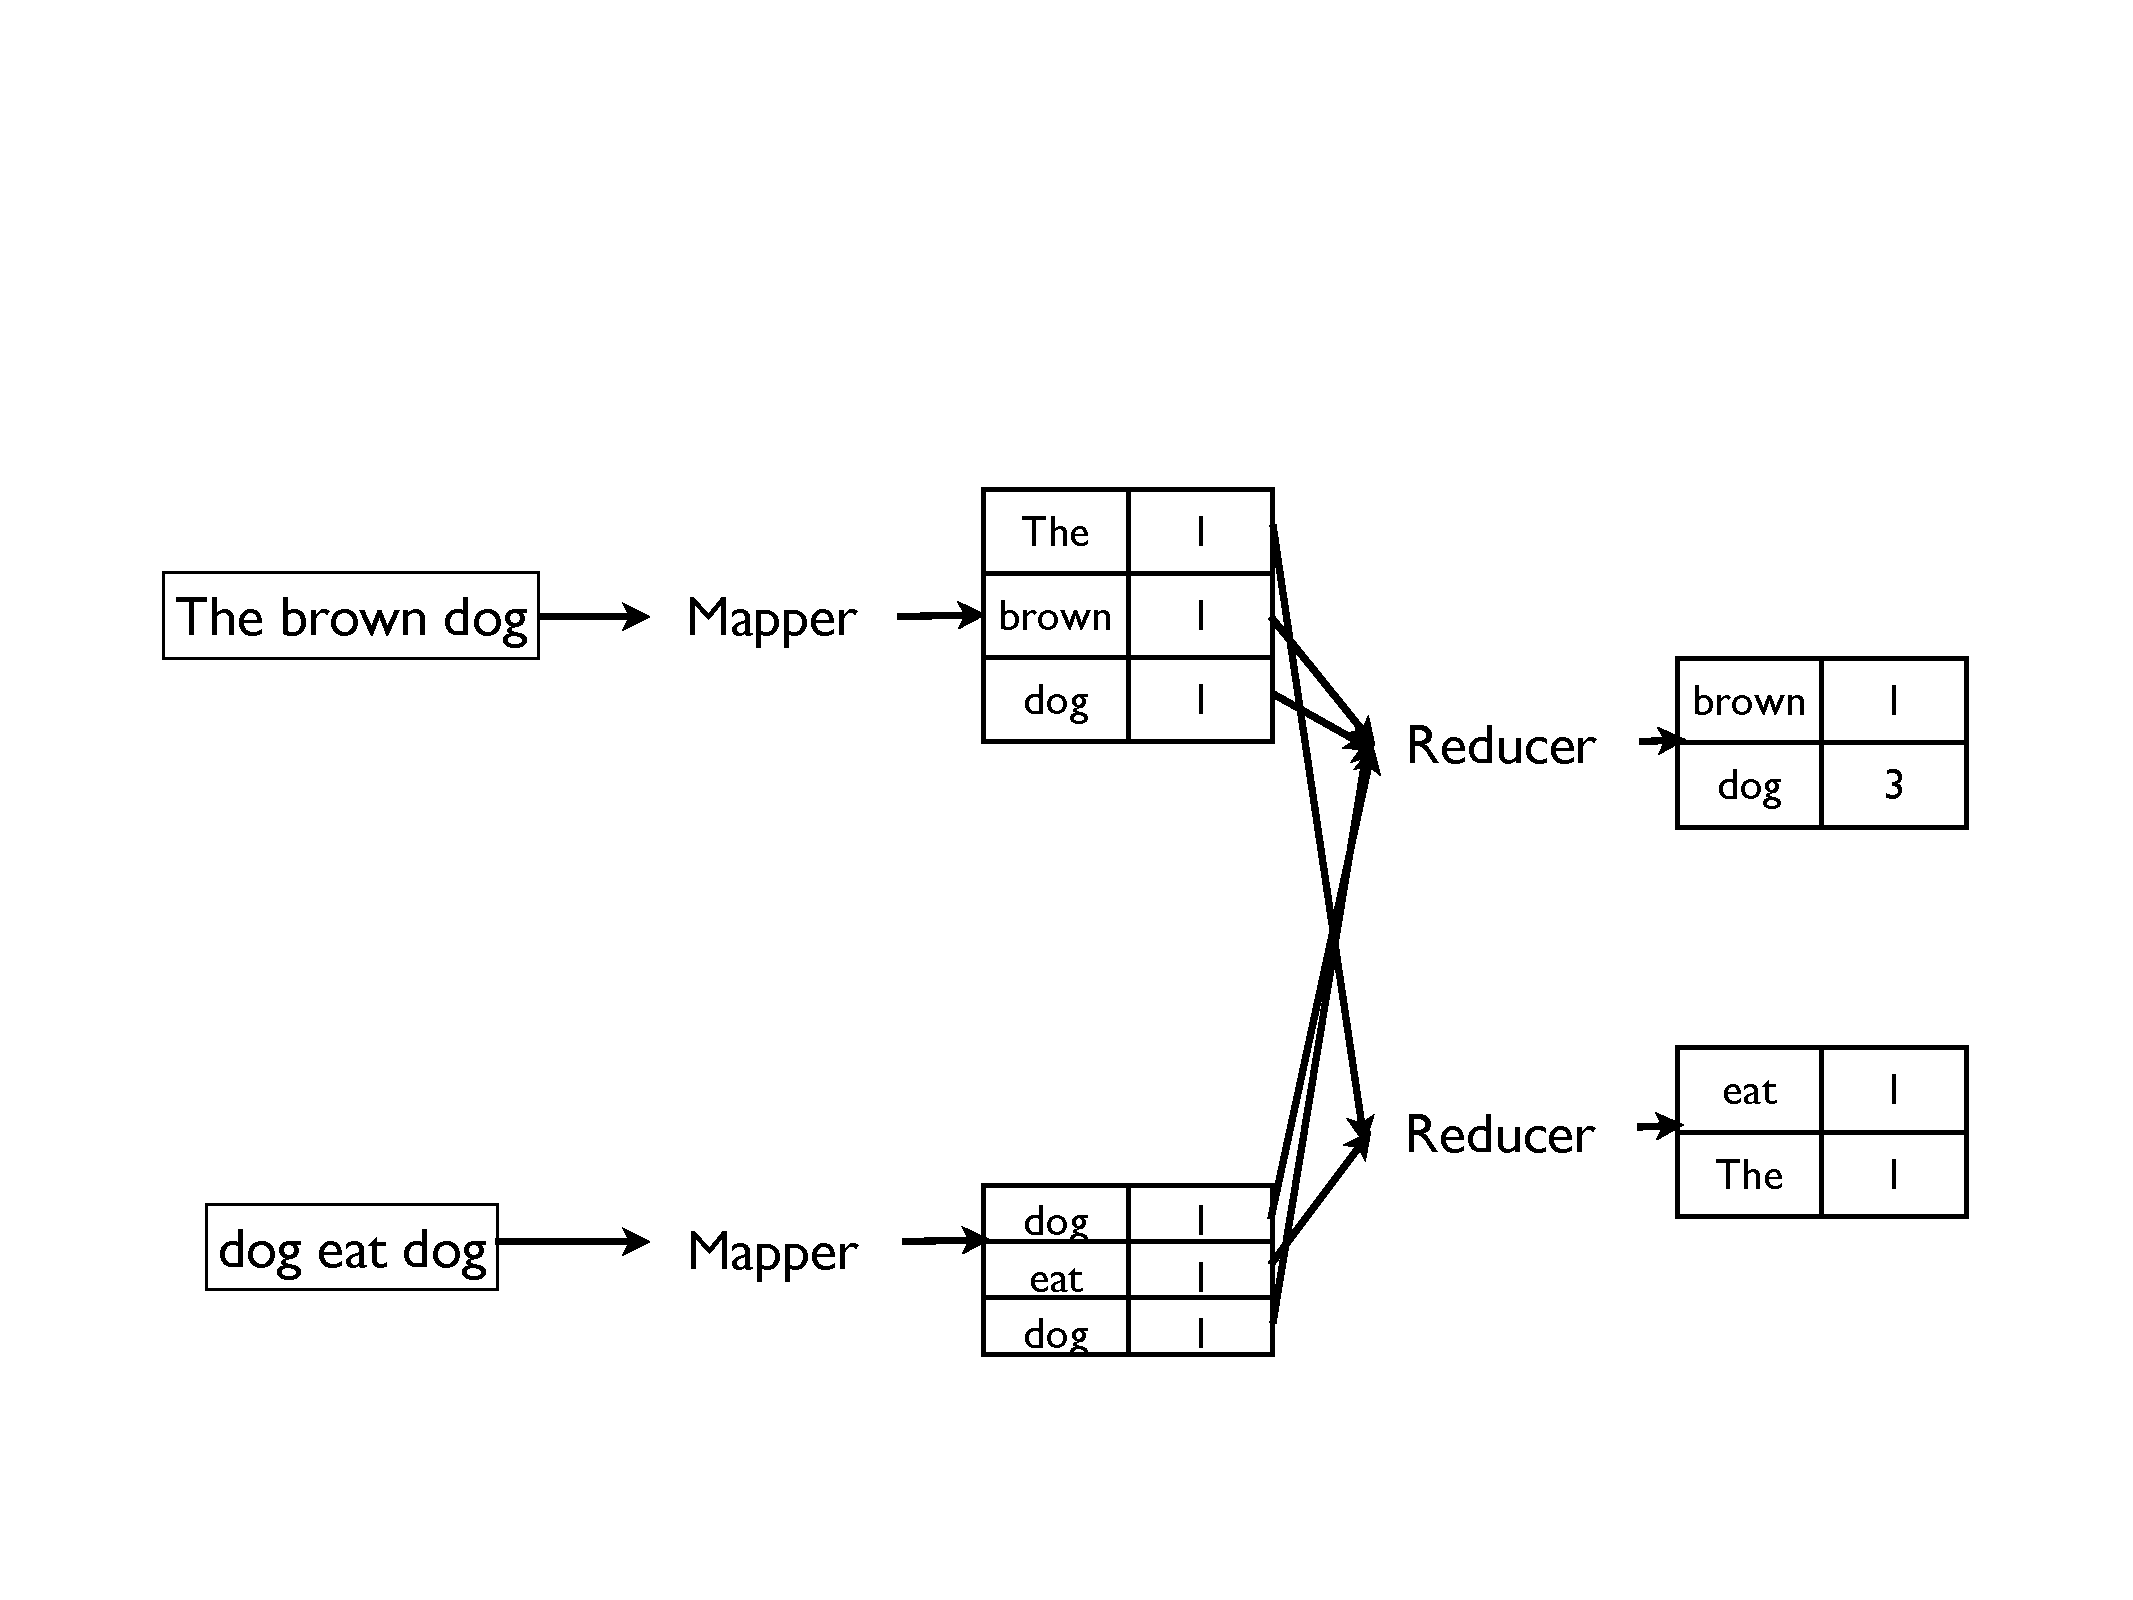
\includegraphics[width=1\textwidth,trim=0in 1in 0in 3in,clip]{figures/mapreduce_example.pdf}
\caption{The word count example MapReduce application. Mappers examine blocks of text data and emit the value one under a key for each word that they encounter. Reducers sum the values they receive for each word, resulting in a count of the number of times each word occurs in the data set.}
\label{mapreduce_example}
\end{figure}

Hadoop is the Apache Software Foundation's open source implementation of the framework described by Google in Dean and Gehemewat's MapReduce paper. It includes an implementation of the MapReduce job scheduler, called the \emph{TaskTracker}, as well as a distributed file system that mimics GFS called HDFS. The open source community has developed Hadoop extensively, with support from many corporations including Yahoo! and Facebook, making it a widely adopted and extended platform for distributed computing.

\section{Uses of Hadoop and MapReduce in Sequencing Tasks}

Now that we understand the components of Hadoop and MapReduce, we can explore its use in sequencing-related bioinformatic tasks. Figure~\ref{bio_hadoop_ecosystem} gives an overview of the published applications of Hadoop to three popular sequencing pipelines: DNA resequencing, RNA-seq, and \emph{de novo} assembly. In some cases, researchers have developed native MapReduce algorithms to solve particular problems. In other instances, Hadoop has been used to run existing tools in parallel; of course, this is only possible when the tasks are embarrassingly parallel at some level. Finally, there are several lower-level APIs, toolkits, and frameworks that have been created in an attempt to ease the development of Hadoop pipelines. These toolkits provide wrappers for reading and writing popular sequencing related file formats, wrappers for commonly used tools, and functions to manipulate short read sequences and alignment records. We will discuss each of these pipelines in more detail in the following sections.

\begin{figure}
\centering
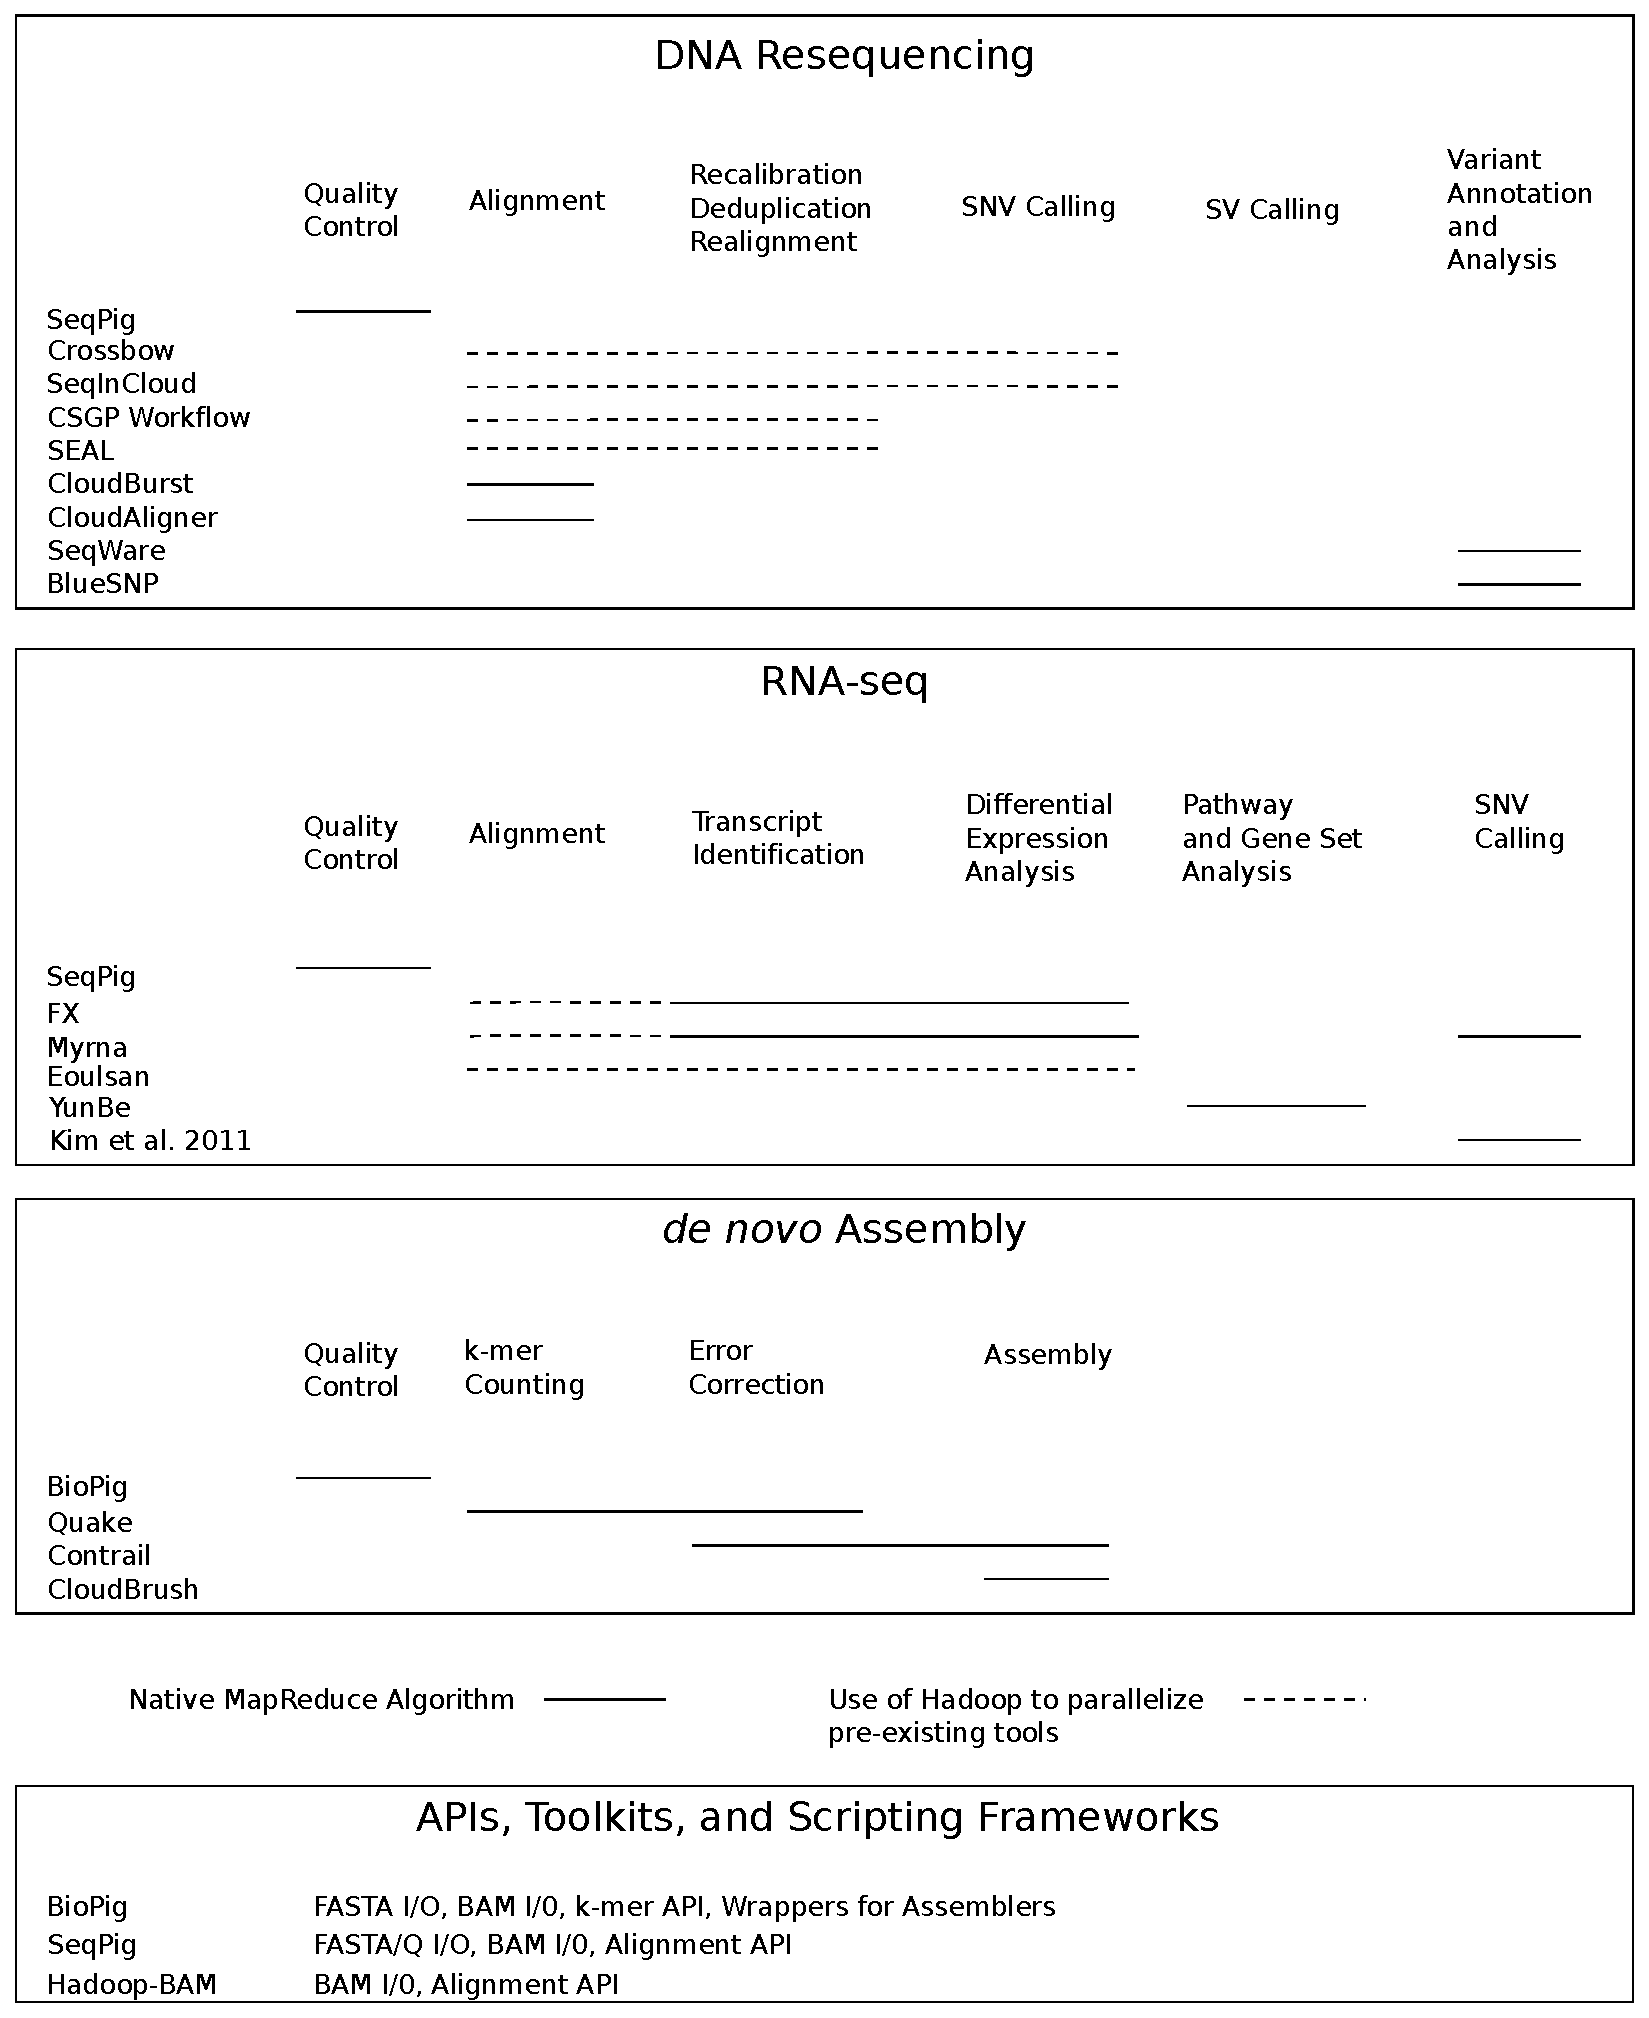
\includegraphics[width=1\textwidth]{figures/bio_hadoop_ecosystem.pdf}
\caption{Hadoop applications to tasks of three popular sequencing analysis pipelines. Solid lines indicate native MapReduce applications developed specifically for Hadoop. Dotted lines indicate pipelines that parallelize the execution of existing tools on splits of the input data using Hadoop. In addition, several toolkits and frameworks are listed that are broadly applicable to many portions of these pipelines.}
\label{bio_hadoop_ecosystem}
\end{figure}

\subsection{DNA Resequencing}

As we discussed in Section~\ref{section_pipelines}, there are multiple steps that are typically part of DNA resequencing pipelines. These steps included quality control analysis, alignment to the genome reference, a series of processes including realignment in problematic regions and removal of duplicate reads, steps to call SNVs and SVs, and finally annotation and analysis of the variants that were discovered. 

A native algorithm for mapping short reads to a reference genome was first demonstrated in Cloudburst~\cite{Schatz:2009p278}. This algorithm creates keys for each k-mer that appears in both the reads and the reference. The reducers then bring together the reads and portions of the reference that match on the same k-mer, and determine whether the match on the seed can be extended to an alignment of the entire read to the reference. Because the read and reference portions are each transferred to the reducers for every single k-mer which appears in them, this algorithm, while accurate, generates large amounts of data that must be shuffled, sorted, and potentially cross the network. Therefore, it is difficult to scale it to very large read sets. This shows the difficulty of designing true MapReduce algorithms that can scale and take advantages of Hadoop's infrastructure. CloudAligner~\cite{Nguyen:2011p1832} uses a similar seed-and-extend algorithm, although the exact details of their map and reduce steps are not specified.

Since short read mapping is an embarrassingly parallel task and highly optimized non-MapReduce alignment tools with full feature sets are readily available, it is more efficient in practice to use the map phase of a Hadoop job to align splits of input reads with existing tools, and then merge results in the reduce phase. SEAL~\cite{Pireddu:2011fj} and the CRS4 Sequencing and Genotyping Platform's CSGP workflow~\cite{Pireddu:2011:MGS:1996092.1996106} are two such pipelines which use the BWA~\cite{Li:2009p836} aligner in each map task. By emitting mappings under a key for the alignment location, they are then able to accomplish the duplicate removal step in the reduce function in a manner similar to that of the popular non-MapReduce tool Picard~\cite{picard}. Similarly, Crossbow~\cite{Langmead:2009p1225} uses Hadoop to parallelize Bowtie~\cite{Langmead:2009p768}. Crossbow then calls single nucleotide variants in the reduce phase using SOAPsnp~\cite{Li:2009p1236}, allowing it to function as a minimum viable pipeline for sequencing. Crossbow also includes infrastructure for running in the Amazon Elastic Compute Cloud, which has contributed to its popularity. SeqInCloud~\cite{nabeel-bicob13-genome-analysis-cloud} similarly combines BWA with the GATK's~\cite{McKenna:2010p1051} realignment and SNV calling steps, along with infrastructure to run in the Microsoft Azure cloud computing platform.

After variant discovery, the usual next step in a resequencing project is to analyze the variants found to detect functional impact (i.e. what genes might be disrupted by the variants found) or to find associations between variants and phenotypes, as in case-control sequencing projects. SeqWare~\cite{Oconnor:2010p1835} uses HBase~\cite{hbase}, a Hadoop database based upon Google's BigTable~\cite{Chang:2008:BDS:1365815.1365816}, to provide functionality to annotate and query the variants. SeqWare uses the genomic coordinates of variants and coverage information as schema keys within HBase's MapReduce queries. BlueSNP~\cite{Huang:2012bb}, meanwhile, implements Hadoop algorithms for finding significant loci and estimating p-values through permutation analysis in genome wide association studies.

To our knowledge, Hadoop/MapReduce have not been used for SV detection. Several non-Hadoop pipelines such as HugeSeq~\cite{Lam:2012jy} and SVMerge~\cite{Wong:2010p1271} use grid scheduling engines like SGE to distribute SV detection tasks across compute clusters. For example, the HugeSeq pipeline is an end-to-end pipeline for DNA resequencing that integrates BreakDancer~\cite{Chen:2009p3}, Pindel~\cite{Ye:2009p2}, CNVnator~\cite{Abyzov:2011bk}, and BreakSeq~\cite{Lam:2010p1383} for SV calling. However, these pipelines can only achieve parallelization by sample or at most by chromosome of the reference, limiting their scalability.

\subsection{RNA-seq}

The goals of RNA-seq are to determine the transcripts and isoforms being expressed, quantify their differential expression, and potentially call DNA variants based on the sequences of the RNA transcripts.  Myrna~\cite{Langmead:2010p1268} and FX~\cite{Hong:2012du} are Hadoop pipelines that execute alignment, transcript identification, and differential expression calculations in multiple Hadoop jobs. Myrna uses Bowtie in each mapper to distribute alignment work across the cluster, and then parallelizes each of the differential expression calculations by first assigning alignments to transcripts, gathering the data by sample to compute normalization factors, and then re-gathering the normalized counts under keys representing transcripts to compute statistics. FX has a less complex workflow, in which alignments are executed in a map-parallel fashion using the GSNAP alignment tool~\cite{Wu:2010p875}, and then has simple steps to count reads by gene for differential expression statistics, and to call SNPs in genes. Both Myrna and FX have infrastructure to automatically create Hadoop clusters in Amazon EC2. Eoulsan~\cite{Jourdren:2012dc} is a very similar workflow, which allows a number of aligners to be used in the mapping step, and then computes read counts per gene in parallel, before computing differential expression statistics outside of the Hadoop environment using existing tools. For use after expression levels have been computed, YunBe~\cite{Zhang:2011p1823} computes statistics to determine whether particular gene pathways have been perturbed in two sets of samples, using a MapReduce strategy where mappers produce expression values from the sample data under keys that represent specific pathways, and reducers aggregate all data for each pathway to determine a ``perturbation statistic'' between sample conditions. Finally, Kim et al.~\cite{Kim2011RNASEQ} described a pipeline for SNV detection from RNA-seq data based on a Hadoop job in which the mappers emit each base and quality score from the aligned reads under a key representing the genomic coordinate, and reducers call the absence or presence of a SNV at each location.

\subsection{\emph{de novo} Assembly}

The third major pipeline for which there has been significant interest in applying Hadoop and MapReduce is \emph{de novo} assembly. Most state-of-the-art algorithms for assembly depend on building large data structures that model the overlaps between reads (in the case of string graph based approaches) or between k-mers found in the reads (in the case of de Bruijn-graph algorithms) as edges in a graph. Given the high depth of coverage that is needed to produce a quality assembly, these graphs become very large, and the need to traverse them requires random rather than sequential access to the data. This would seem to make the problem a poor fit for Hadoop, which is optimized for sequential access of large data sets on commodity hardware. Nevertheless, several groups have attempted to create assembly algorithms using MapReduce. Contrail~\cite{schatz2010novo} builds a de Bruijn graph by emitting each pair of consecutive k-mers from the reads as a key-value pair to form a k-mer adjacency matrix. CloudBrush~\cite{Chang:2012hd} uses a ``prefix-and-extend'' strategy~\cite{10.1109/CLOUD.2012.123}, in which all k-mers that appear in the reads are used as keys, with the reads themselves as values. Extension procedures then test whether the k-mer is the prefix of one of the reads and the suffix of another. Both of these tools have then developed MapReduce procedures for graph pruning and traversal that are necessary to produce contigs from their respective graph data structures. Finally, some helpful read pre-processing steps for assembly have been implemented in Hadoop: Quake~\cite{Kelley:2010kg} is a widely used MapReduce k-mer counter, and BioPig~\cite{Nordberg:2013ka} also contains facilities for k-mer analysis of large read sets.

\subsection{Frameworks and Toolkits}

In addition to the pipelines listed above, recently several sequencing-related frameworks and toolkits have been created to ease the development of Hadoop applications. These tools include APIs and library code to handle reading from and writing to files in popular sequencing data formats. For example, Hadoop-BAM~\cite{Niemenmaa:2012hu} allows manipulation of data in the SAMtools~\cite{Li:2009vz} binary alignment format BAM. Two libraries, SeqPig~\cite{Schumacher:2013kh} and BioPig~\cite{Nordberg:2013ka}, were also recently published that provide file formats and commonly used functions in the Apache Pig~\cite{pig} environment, which provides a high-level programming language called Pig Latin that allows easy expression of simple data analysis tasks. These libraries allow for rapid development of scripts that gather statistics on read and alignment data sets, and Pig automatically optimizes their execution by translating them into one or more MapReduce jobs. 

\subsection{Other uses of Hadoop and MapReduce}

Although not implemented in Hadoop, the very widely used Genome Analysis Toolkit~\cite{McKenna:2010p1051} (GATK) implements many sequencing and variant calling functions using a MapReduce programming model. Although it currently can only distribute tasks across clusters using traditional grid engines, future versions of this package may be re-implemented to use Hadoop. Other notable sequencing applications that have been implemented in Hadoop include ChIP-seq peak calling~\cite{Feng:2011p1228}, and computing genome mappability scores~\cite{Lee:2012bk}. 

\section{MapReduce Constraints on SV Algorithms}

To this point, we know of no Hadoop-based SV detection algorithms. This may be because the need to separate logic into mappers and reducers makes it difficult to implement traditional RP-based SV detection approaches in MapReduce, particularly given the global clustering of paired end mappings at the heart of many RP approaches. MapReduce algorithms, by contrast, excel at conducting many independent calculations in parallel. The sequencing applications that have been implemented in MapReduce succeed by dividing processing into a series of local computation, for example calling a SNV at a particular location in the genome given the reads that cover it, to use the example of Crossbow~\cite{Langmead:2009p1225}, the most widely accepted sequencing MapReduce algorithm. As we noted in Chapter~\ref{chap_related_work}, SV approaches that are similarly based on local computations have been described: the RP-based SV callers MoDIL~\cite{Lee:2009da} and forestSV~\cite{Michaelson:2012fj} try to solve the SV detection problem by computing scores or features along the genome and then producing SV predictions from those features in a post-processing step. In the remainder of this chapter, we formalize this idea and develop it as a potential framework for implementing SV detection algorithms in MapReduce.

\section{A General MapReduce SV Detection Algorithm}\label{section_general_algo}

Using this strategy, we have developed a conceptual algorithmic framework for SV detection in MapReduce, which is outlined in Algorithm~\ref{cb_algo}. This framework divides processing into three separate MapReduce jobs: an alignment job, a feature computation job, and an SV calling job. The overall workflow of the algorithm and its implementation on a compute cluster or cloud is summarized in Figure~\ref{cloudbreak_workflow}.

\begin{figure}
\centering
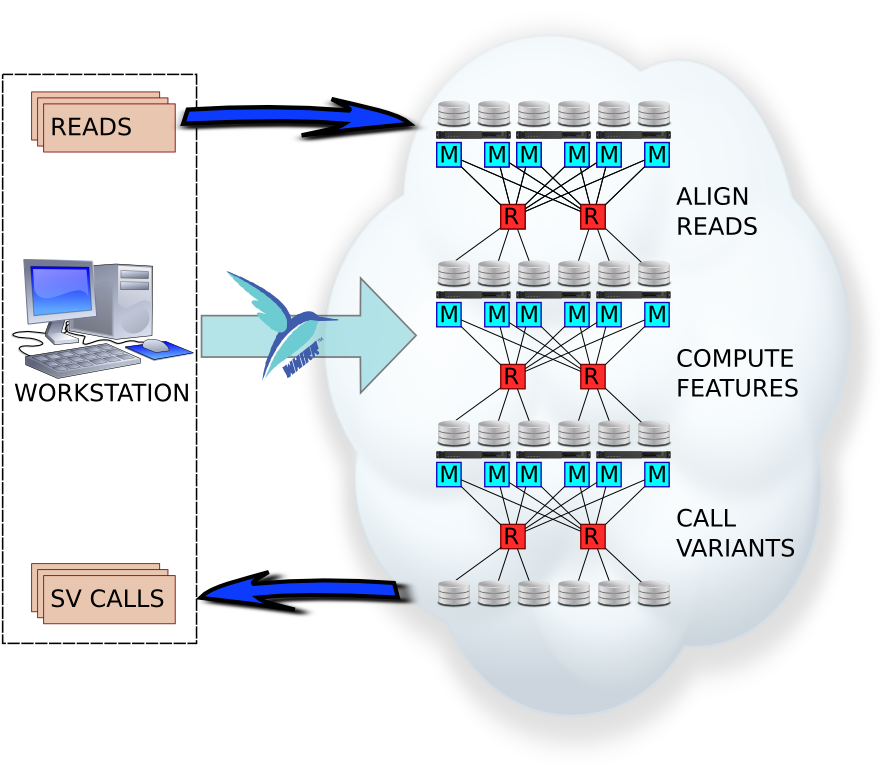
\includegraphics[width=.8\textwidth]{figures/workflow_with_whirr.png}
\caption{An overview of the steps of the MapReduce SV detection workflow. Reads are first uploaded to a Hadoop cluster from local storage. Processing is then then divided into three MapReduce jobs: 1) Mapping with sensitive settings. 2) Computation of features across the genome. 3) Calling structural variations based on the features computed in the previous step. Finally, SV predictions can be downloaded from the Hadoop cluster and examined and annotated. Cloudbreak can also use the Apache Whirr library to automatically provision Hadoop clusters on and deploy data to cloud providers such as Amazon Elastic Compute Cloud.}
\label{cloudbreak_workflow}
\end{figure}


The \textsc{Align Reads} job uses existing alignment tools to discover mapping locations for each read pair. Aligners can be executed to report multiple possible mappings for each read, or only the best possible mapping. Given a set of read pairs, each of which consists of a read pair identifier $rpid$ and two sets of sequence and quality scores $<s,q>$, each mapper aligns each pair end set $<s,q>$ in either single- or paired end mode and emits possible mapping locations under the $rpid$ key. Reducers then collect the alignments for each paired end, making them available under one key for the next job. 

In the \textsc{Compute Features} job, we compute a set of features for each location in the genome. To begin, we tile the genome with small fixed-width, non-overlapping intervals. For the experiments reported in Chapter~\ref{chap_cloudbreak_eval} we use an interval size of 25bp (see Section~\ref{section_window_size} for an exploration of the effects of different window sizes on accuracy and runtime). Let $L = \left\{l_1,l_2,\ldots,l_N\right\}$ be the set of intervals covering the entire genome. Let $R^1 = \left\{r^{1}_{1},r^{1}_{2},\ldots,r^{1}_{M}\right\}$ and $R^2 = \left\{r^{2}_{1},r^{2}_{2},\ldots,r^{2}_{M}\right\}$ be the input set of paired reads. Let $A^1 = \left\{a^{1}_{m,1},a^{1}_{m,2},\ldots,a^{1}_{m,K}\right\}$ and $A^2 = \left\{a^{2}_{m,1},a^{2}_{m,2},\ldots,a^{2}_{m,L}\right\}$ be the set of alignments for the left and right reads from read pair $m$. For any given pair of alignments of the two reads in a read pair, $a^{1}_{m,i}$ and $a^{2}_{m,j}$, let the $\textrm{ReadPairInfo } rpi_{m,i,j}$ be information about the pair relevant to detecting SVs, e.g. the fragment size implied by the alignments and the likelihood that the alignments are correct. We then leave two functions to be implemented depending on the application:
\begin{flalign*}
 \textsc{Loci } :& \langle a^{1}_{m,i},a^{2}_{m,j} \rangle \rightarrow L_m \subseteq L \\
 \Phi :& \left\{\textrm{ReadPairInfo }rpi_{m,i,j}\right\} \rightarrow \mathbb{R}^N \\
\end{flalign*}

The first function, \textsc{Loci}, maps an alignment pair to a set of genomic locations to which it is relevant for SV detection; for example, the set of locations overlapped by the internal insert implied by the read alignments.  We optimize this step by assuming that if there exist concordant mappings for a read pair, defined as those where the two alignments are in the proper orientation and with an insert size within three standard deviations of the expected library insert size, one of them is likely to be correct and therefore we do not consider any discordant alignments of the pair. The second function, $\Phi$, maps a set of ReadPairInfos relevant to a given location to a set of real-valued vectors of features useful for SV detection. 

Finally, the third MapReduce job, \textsc{Call Variants}, is responsible for making SV calls based on the features computed at each genomic location. It calls another application-specific function: 

 \[ \textsc{PostProcess} : \left\{\phi_1,\phi_2,\ldots,\phi_N\right\} \rightarrow \left\{\langle  \textrm{SVType } s, l_{start}, l_{end} \rangle\right\} \]

This function maps the sets of features for related loci into a set of SV calls characterized by their type $s$ (i.e Deletion, Insertion, etc.) and their breakpoint locations $l_{start}$ and $l_{end}$. We parallelize this job in MapReduce by making calls for each chromosome in parallel, which we achieve by associating a location and its set of features to its chromosome in the map phase, and then making SV calls for one chromosome in each reduce task.

\begin{algorithm}
\algrenewcommand\algorithmicprocedure{\textbf{job}}
 \begin{algorithmic}[1]
 \Procedure{Alignment}{}
 \Function{Map}{$\textrm{ReadPairId }rpid, \textrm{ReadId }r, \textrm{ReadSequence }s, \textrm{ReadQuality }q$}
 \ForAll{$ \textrm{Alignments }a \in \textsc{Align}(<s,q>)$}
 \State $\textsc{Emit}(\textrm{ReadPairId }rpid, \textrm{Alignment }a)$
 \EndFor
 \EndFunction
 \Function{Reduce}{$\textrm{ReadPairId }rpid, \textrm{Alignments }a_{1,2,\ldots}$}
 \State $\textrm{AlignmentPairList }ap \gets \textsc{ValidAlignmentPairs}(a_{1,2,\ldots})$
 \State $\textsc{Emit}(\textrm{ReadPairId }rp, \textrm{AlignmentPairList } ap)$
 \EndFunction
 \EndProcedure

 \Procedure{Compute SV Features}{}
 \Function{Map}{$\textrm{ReadPairId }rp, \textrm{AlignmentPairList }ap$}
 \ForAll{$ \textrm{AlignmentPairs }<a_1,a_2> \in ap$}
 \ForAll{$ \textrm{GenomicLocations }l \in \textsc{Loci }(a_1,a_2)$}
 \State $ \textrm{ReadPairInfo }rpi \gets <\textrm{InsertSize}(a_1,a_2), \textrm{AlignmentScore}(a_1,a_2)>$
 \State $\textsc{Emit}(\textrm{GenomicLocation }l, \textrm{ReadPairInfo }rpi)$
 \EndFor
 \EndFor
 \EndFunction
 \Function{Reduce}{$\textrm{GenomicLocation }l, \textrm{ReadPairInfos }rpi_{1,2,\ldots}$}
 \State $\textrm{SVFeatures } \phi_l \gets \Phi(\textrm{InsertSizes }i_{1,2,\ldots}, \textrm{AlignmentScores }q_{1,2,\ldots})$
 \State $\textsc{Emit}(\textrm{GenomicLocation }l, \textrm{SVFeatures } \phi_l)$
 \EndFunction
 \EndProcedure

 \Procedure{Call SVs}{}
 \Function{Map}{$\textrm{GenomicLocation }l, \textrm{SVFeatures } \phi_l$}
 \State $\textsc{Emit}(\textrm{Chromosome}(l), <l,\phi_l>)$
 \EndFunction
 \Function{Reduce}{$\textrm{Chromosome }c, \textrm{GenomicLocation } l_{1,2,\ldots},\phi_{1,2,\ldots}$}
 \State $\textrm{StructuralVariationCalls } svs_c \gets \textsc{PostProcess }(\phi_{1,2,\ldots})$
 \EndFunction
 \EndProcedure
 \end{algorithmic}
\caption{The algorithmic framework for SV calling in MapReduce.}
\label{cb_algo}
\end{algorithm}

\section{Discussion}\label{section_framework_discussion}

The framework that we have just described is agnostic to the type of structural variations that the user wishes to detect. In the next chapter, we describe Cloudbreak, our implementation of this framework that identifies small deletions and insertions. To do so, it defines the relevant information from each pair (the ReadPairInfo) as information about the insert size implied by the mapping of the paired reads, sends them to every location which is spanned by that read pair in the reference genome, and then computes features from them by modeling the expected distribution of insert sizes at each location with a Gaussian Mixture Model. We demonstrate some of the strengths of this particular implementation in Chapter~\ref{chap_cloudbreak_eval}. However, we believe that this general framework could be applied to many other SV detection problems. For example, to detect inversions, one might define a different ReadPairInfo for each pair that includes information about the orientation of the mappings. Translocation detection programs might emit ReadPairInfos that contain information about the chromosomes linked to by interchromosomal mappings, which the $\Phi$ function would then cluster to see if a preponderance of those mappings point to the same breakpoint location. In addition to paired mapping locations, it would also be possible to design ReadPairInfo and feature function definitions that allowed the computation of read depth or split read related features, enabling the integration of more of the signals available in the data set. We will explore one possible way to integrate disparate features such as these in Chapter~\ref{chap_crf}. Use of the Hadoop/MapReduce computing framework would ensure that any of these applications, if carefully designed, could enjoy the benefits of redundancy, data locality, and scalability we described in Section~\ref{section_hadoop_description}, and therefore will be able to grow to meet the rising demands of genomics applications in the near future.

\chapter{Cloudbreak}\label{chap_cloudbreak_impl}

In the previous chapter, we described and formalized a general strategy for building SV detection algorithms in MapReduce and Hadoop. In this chapter, we describe an software package, Cloudbreak, that we have developed using this algorithmic framework. To build Cloudbreak, we implemented the infrastructure necessary to support the algorithmic framework we described in Section~\ref{section_general_algo}, and also provided implementations of the three application-specific functions we described there. Here we will describe this implementation, as well as our choices for the three user-defined functions we specified in the framework definition, and additional functionality we developed to genotype calls and to facilitate the deployment of Cloudbreak on public cloud platforms including Amazon's EC2. In Chapter~\ref{chap_cloudbreak_eval}, we will provide an evaluation of the algorithm's accuracy and performance characteristics.

\section{Variant types detected}

Cloudbreak is our implementation of a detection algorithm for genomic deletions (40bp-25,000bp) and small insertions based on examining the insert sizes of paired end mappings. We chose this application because small deletions in the range of 50bp to 150bp are particularly difficult to detect using many existing SV algorithms~\cite{Alkan:2011p547,Mills:2011fi}. This is because most read-pair based algorithms use a hard cutoff based on the variance of the fragment size distribution to select discordant read pairs, as described in Section~\ref{section_read_pair}. By taking advantage of many compute cores using MapReduce, we can design an algorithm that considers all of available data (both concordant and discordant read pairs) in a generative statistical framework, as we will describe in Section~\ref{section_user_defined_functions}.

\section{Framework infrastructure}

In addition to the specific algorithm for detecting deletions and insertions (which take the form of implementations of the user-defined functions we described in the previous chapter), the Cloudbreak package also contains the infrastructure necessary to implement the three MapReduce jobs defined in our MapReduce algorithmic framework. Providing a fully featured, multi-job Hadoop application requires several implementation decisions:

\begin{itemize}
\item \textbf{Programming language and method of interacting with Hadoop.} Hadoop applications can be developed in several ways. A native application is written in Java and directly uses the Hadoop application programming interface (API) to start jobs, implement Map and Reduce functions, and set advanced Hadoop configurations. Alternatively, applications can be developed in any language using the Hadoop \emph{streaming} interface, as long as the input to and output from all map and reduce tasks is textual and certain conventions are followed with respect to data format. Finally, for C/C++ applications, the Hadoop \emph{pipes} interface can be used to marshal input and output data from tasks. Each method has its own advantages and disadvantages. Native applications constrain the developer to Java but enjoy the best performance when the jobs are data intensive rather than CPU bound~\cite{Ding:2011:MCM:2103380.2103444}. Streaming applications allow greater programming language flexibility but make it somewhat more difficult to organize complex applications and take advantage of advanced Hadoop features. Pipes, meanwhile, allow for maximum performance for CPU intensive applications. We opted to develop Cloudbreak as a native application to take advantage of the tight integration with the Hadoop API improved I/O performance on data intensive portions of the workflow. For the \textsc{Align Reads} job, which executes existing short-read alignment tools, a mapper class written in Java invokes the external tools using the system runtime environment.

\item \textbf{File formats and compression.} Hadoop applications usually store their data in HDFS in text format or in sequence files, a binary format that allows numeric or complex data types to be stored in a key-value pair structure easily accessed by Hadoop. In addition, varying levels of compression can be used, although only certain compression types allow Hadoop to automatically split large files by HDFS blocks for processing by different map tasks, which is a key consideration for building fully parallelized applications. Cloudbreak uses sequence files for input and intermediate files, although for alignments the values are stored as text strings containing full records in the Sequence Alignment Map (SAM) format~\cite{Li:2009vz}, to allow for easy exports of data. For compression we use the Snappy~\cite{snappy} compressor/decompressor (codec), a compression scheme developed at Google which aims for reasonable file size reduction with very fast compression and decompression speeds. This makes it ideal for data-intensive Hadoop applications. Given that the output data from the \textsc{Align Reads} job is alignment records, a future implementation goal is to switch to using Hadoop-BAM~\cite{Niemenmaa:2012hu}, a library for storing SAM/BAM records efficiently in HDFS; Hadoop-BAM did not posses necessary functionality at the time of Cloudbreak's initial implementation and so we proceeded with a text-based representation of alignment records.

\item \textbf{Distribution of auxiliary files.} In some cases all tasks require access to large input files, such as genome reference indices for alignment, or genome annotation files. Hadoop offers a \emph{distributed cache} service, which places copies of the files on each node that will host tasks for the job so that they will not all need to copy the files over the network. Cloudbreak makes use of the distributed cache to distribute index and annotation files, as well as the alignment executables for the \textsc{Align Reads} job.
\end{itemize}

Our implementation of the \textsc{Align Reads} job contains wrappers to execute the aligners BWA \cite{Li:2009p836}, GEM \cite{MarcoSola:2012hm}, Novoalign \cite{novoalign}, RazerS 3 \cite{Weese:2012by}, mrFAST \cite{Alkan:2009cr}, and Bowtie 2 \cite{Langmead:2012jh}. This job can also be skipped in favor of importing a pre-aligned BAM file directly into HDFS. The code is structured in such a way that to add a new aligner, developers would simply create a class that finds the necessary index files in the distributed cache and determines the proper command line parameters for aligner execution, and parses the aligner output if it is in a non-standard format.

Cloudbreak can be executed on any Hadoop cluster; Hadoop abstracts away the details of cluster configuration, making distributed applications portable. We deployed Cloudbreak on an internal 56-node cluster running the Cloudera CDH3 Hadoop distribution, version 0.20.2-cdh3u4. In addition, Cloudbreak can create and operate on Hadoop clusters in the Amazon compute cloud (see Section~\ref{section_cloud_whirr}).

The source code and user manual for Cloudbreak are publicly available at \url{https://github.com/cwhelan/cloudbreak}. We hope that by publishing under an open-source license, we will facilitate the adoption of our Cloudbreak implementation, as well as provide a base from which other computational researchers can develop their own SV detection algorithms for Hadoop.

\section{Implementation of a MapReduce SV Algorithm}\label{section_user_defined_functions}

In Section~\ref{section_general_algo}, we described three user-defined functions that can be implemented to create an SV detection application in our MapReduce framework. These functions were named \textsc{Loci}, $\Phi$, and \textsc{PostProcess}. These functions map aligned read pairs to locations on the genome to which they are relevant, compute a set of local features for each genomic location based on the relevant read pairs, and call variants based on the features computed for neighboring genomic locations. Cloudbreak contains implementations of these functions that combine to allow it to detect deletions (of size 40bp-25,000bp) and insertions. A detailed description of each of these implementations appears below, and an illustration of each phase of the Cloudbreak algorithm working on a simple example in MapReduce is shown in Figure \ref{cloudbreak_example}.

\begin{figure}
\centering
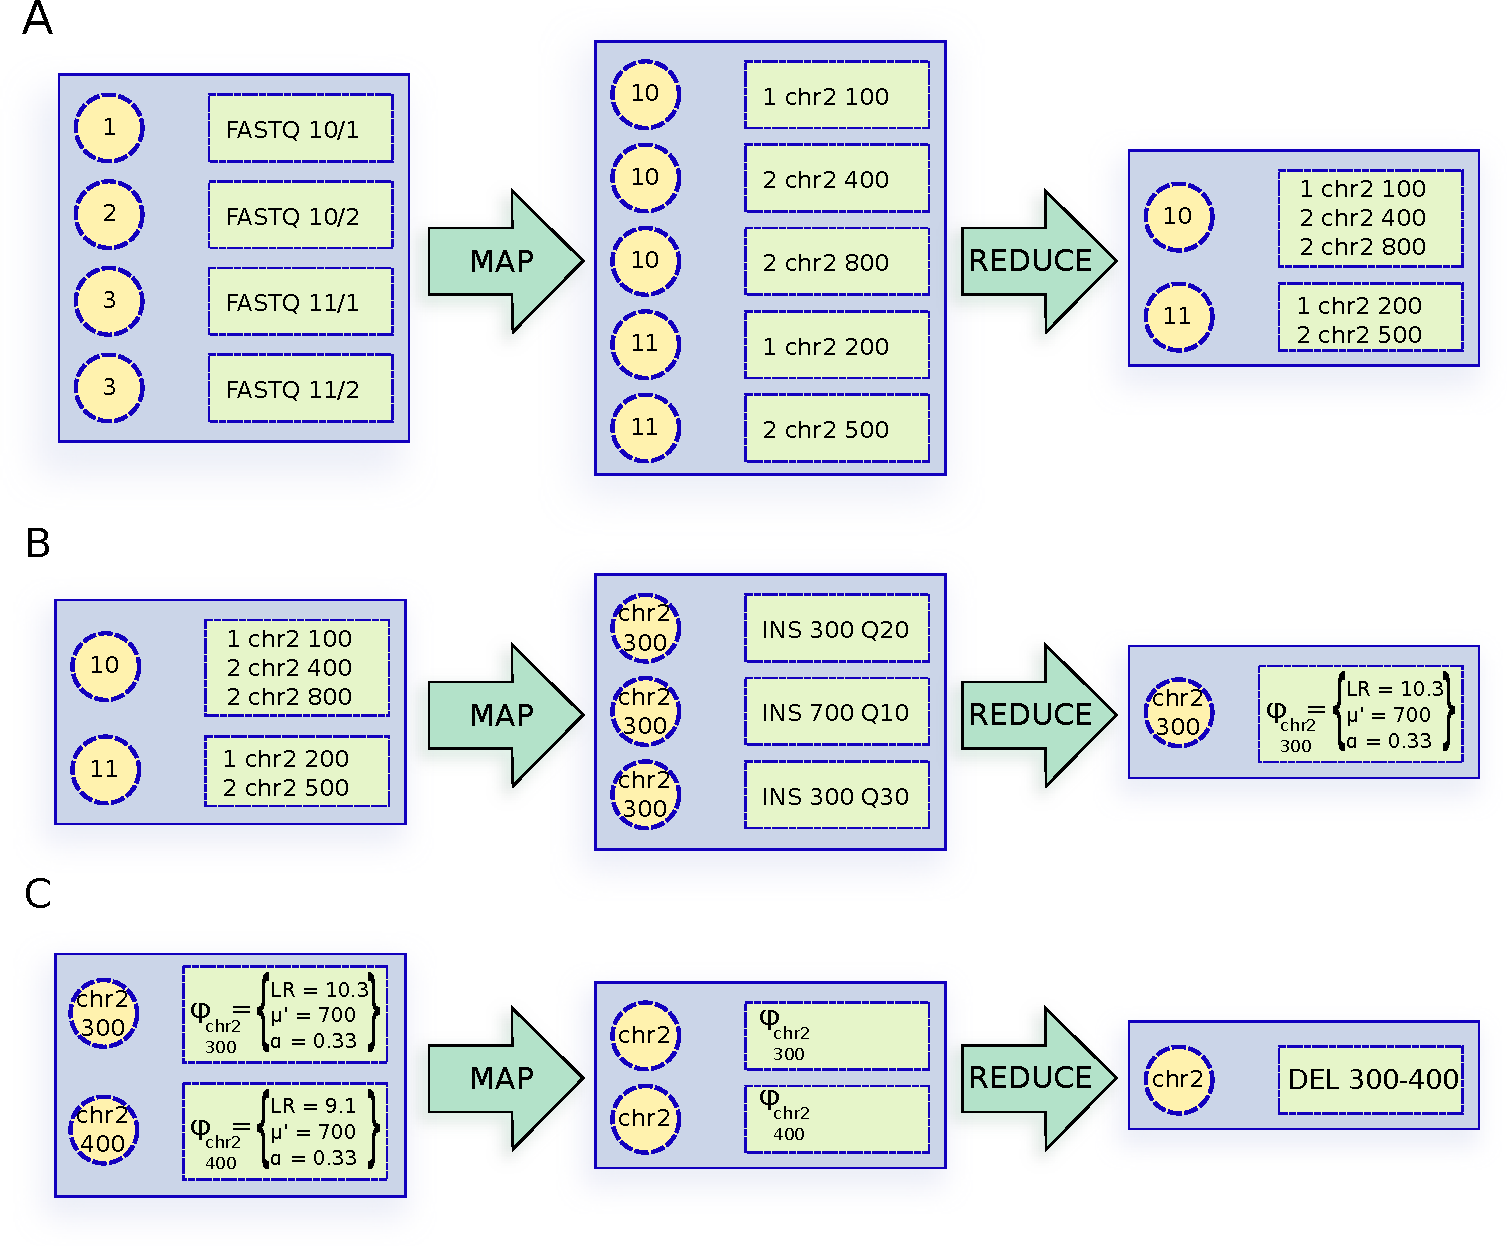
\includegraphics[width=.9\textwidth]{/users/cwhelan/Documents/svpipeline/figures/cloudbreak_mapred_diagram.pdf}
\caption{An Example of the Cloudbreak deletion and insertion detection algorithm running in MapReduce. A) In the first MapReduce job, mappers scan input reads in FASTQ format and execute an alignment program in either paired-end or single-ended mode to generate read mappings. Reducers gather all alignments for both reads in each pair. B) In the second MapReduce job, mappers first emit information about each read pair (in this case the insert size and quality) under keys indicating the genomic location spanned by that pair. Only one genomic location is diagrammed here for simplicity. Reducers then compute features for each location on the genome by fitting a GMM to the distribution of spanning insert sizes. C) Mappers group all emitted features by their chromosome, and reducers find contiguous blocks of features that indicate the presence of a variant.}
\label{cloudbreak_example}
\end{figure}

\begin{description}
\item[\sc{Loci}] Because we are detecting deletions and short insertions, we map ReadPairInfos from each possible alignment to the genomic locations overlapped by the implied internal insert between the reads. For efficiency, we define a maximum detectable deletion size of 25,000bp, and therefore alignment pairs in which the ends are more than 25kb apart, or in the incorrect orientation, map to no genomic locations. In addition, if there are multiple possible mappings for each read in the input set, we optimize this step by assuming that if there exists a concordant mapping for a read pair, defined as a mapping pair in which the two alignments are in the proper orientation and with an insert size within three standard deviations of the expected library insert size, it is likely to be correct and therefore we do not consider any discordant alignments of the pair.

\item[$\Phi$] To compute features for each genomic location, we follow the mixture of distributions approach (see Section~\ref{section_mixture_of_distributions}) first described by Lee et al.~\cite{Lee:2009da}, who observed that if all mappings are correct, the insert sizes implied by mappings which span a given genomic location should follow a Gaussian mixture model (GMM) whose parameters depend on whether a deletion or insertion is present at that locus. Figure~\ref{insert_size_mixes} shows several examples of the mixtures observed for various types of variants. If there is no indel, the insert sizes implied by spanning alignment pairs should follow the distribution of actual fragment sizes in the sample, which is typically modeled as normally distributed with mean $\mu$ and standard deviation $\sigma$. If there is a homozygous deletion or insertion of length $l$ at the location, $\mu$ should be shifted to $\mu + l$, while $\sigma$ will remain constant. Finally, in the case of a heterozygous event, the distribution of insert sizes will follow a mixture of two normal distributions, one with mean $\mu$, and the other with mean $\mu + l$, both with an unchanged standard deviation of $\sigma$, and mixing parameter $\alpha$ that describes the relative weights of the two components. The features generated for each location $l$ include the log-likelihood ratio of the filtered observed data points under the fit GMM to their likelihood under the distribution $N(\mu,\sigma)$, the final value of the mixing parameter $\alpha$, and $\mu'$, the estimated mean of the second GMM component. 

The choice of a mixture of distributions model has several benefits. Firstly, it is a generative model for the entire data set, including concordant and discordant read pairs. This removes the need to set hard thresholds that define discordant read pairs, and allows the detection of smaller variants given a tight enough insert size distribution. Second, the parameters that are estimated can be used to refine and classify predictions. For example, the mixing parameter $\alpha$ can be used to genotype variants, as we will describe in Section~\ref{section_genotyping}. In addition, the estimated $\mu'$ parameter gives a prediction for how many genomic locations the variant might cover, which we leverage in the \textsc{PostProcess} function described below to integrate local features into variant calls.

To implement our model, at each genomic location we fit the parameters of the GMM using the Expectation-Maximization algorithm. Let $Y = y_{1,2, \ldots m}$ be the observed insert sizes at each location after filtering, and say the library has mean fragment size $\mu$ with standard deviation $\sigma$. Because the mean and standard deviation of the fragment sizes are selected by the experimenter and therefore known \emph{a priori} (or at least easily estimated based on a sample of alignments), we only need to estimate the mean of the second component at each locus, and the mixing parameter $\alpha$. Therefore, we initialize the two components to have means $\mu$ and $\bar{Y}$, set the standard deviation of both components to $\sigma$, and set $\alpha = .5$. In the E step, we compute for each $y_i$ and GMM component $j$ the value $\gamma_{i,j}$, which is the normalized likelihood that $y_i$ was drawn from component $j$. We also compute $n_j = \sum_i{\gamma_{i,j}}$, the relative contributions of the data points to each of the two distributions. In the M step, we update $\alpha$ to be $n_2 - \left|Y\right|$, and set the mean of the second component to be $\frac{\sum_m{\gamma_{m,2}y_m}}{n_2}$. We treat the variance as fixed and do not update it, since under our assumptions the standard deviation of each component should always be $\sigma$. We repeat the E and M steps until convergence, or until a maximum number of steps has been taken. Prior to fitting the GMM at each location, we attempt to filter out incorrect mappings for that location using an outlier-detection based clustering scheme and an adaptive mapping quality cutoff; see Section~\ref{section_incorrect_and_ambiguous_mappings} for details.

\item[\sc{PostProcess}] The third MapReduce job is responsible for making SV calls based on the features defined above. We convert our features along each chromosome to insertion and deletion calls by first extracting contiguous genomic loci where the log-likelihood ratio of the two models is greater than a given threshold. To eliminate noise we apply a median filter with window size 5. We end regions when $\mu'$ changes by more than 60bp ($2\sigma$), and discard regions where the average value of $\mu'$ is less than $\mu$ or where the length of the region differs from $\mu'$ by more than $\mu$.
\end{description}

\begin{figure}
\centering
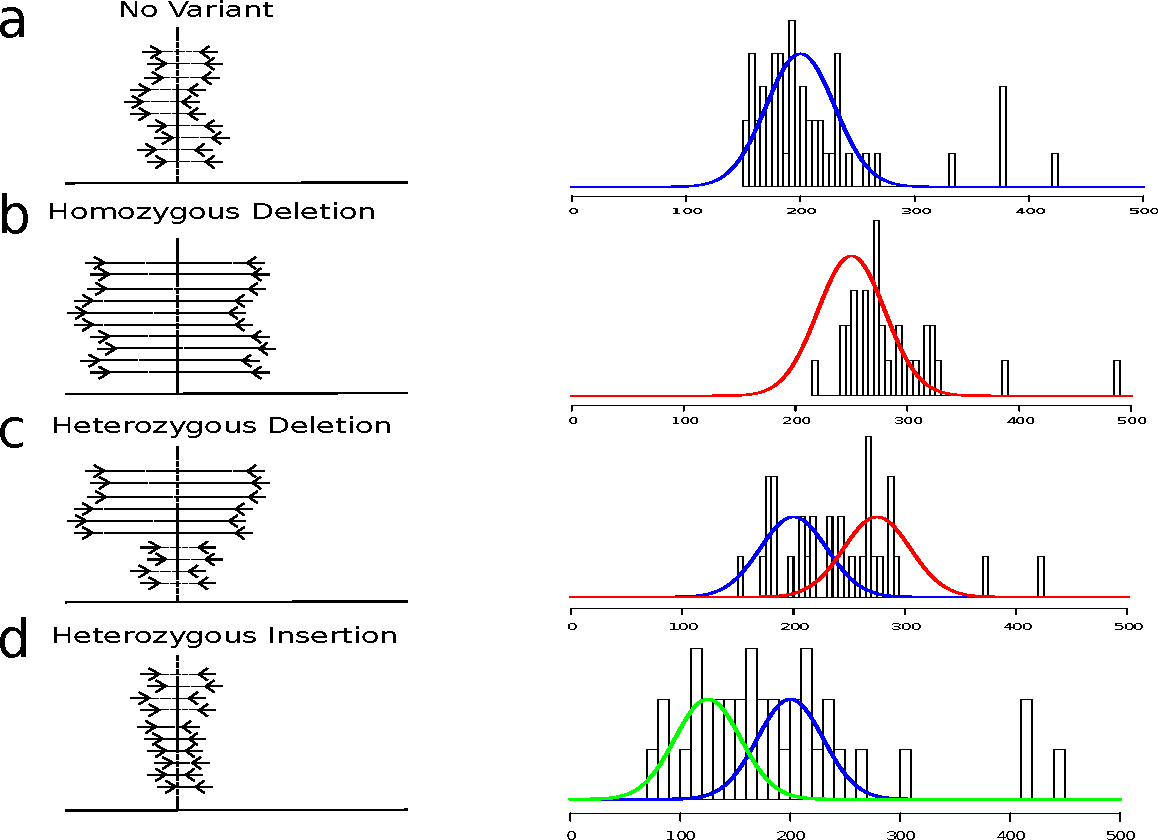
\includegraphics[width=.9\textwidth]{figures/insert_size_mixtures.pdf}
\caption{Illustration of insert size mixtures at individual genomic locations. A) there is no variant present at the location indicated by the vertical line (left), so the mix of insert sizes (right) follows the expected distribution of the library centered at 200bp, with a small amount of noise coming from low-quality mappings. B) a homozygous deletion of 50bp at the location has shifted the distribution of observed insert sizes. C) A heterozygous deletion at the location causes a mixture of normal and long insert sizes to be detected. D) A heterozygous small insertion shifts a portion of the mixture to have lower insert sizes.}
\label{insert_size_mixes}
\end{figure}

\section{Filtering Incorrect and Ambiguous Mappings}\label{section_incorrect_and_ambiguous_mappings}

One of our goals in developing Cloudbreak was to see if the use of distributed computing in the MapReduce framework would allow us to develop an algorithm that could process multiple mappings for ambiguously mapped reads in a reasonable amount of time, especially because the size of the dataset can grow very large if many possible mappings are kept for all ambiguous reads. Most SV detection tools that use multiple mappings attempt to identify the correct mapping for each ambiguously mapped pair; for example, GASVPro~\cite{Sindi:2012kk} uses an MCMC approach to sample from the distribution of possible mapping locations for each read, and VariationHunter~\cite{Hormozdiari:2009p284} attempts to assign mappings to reads through a combinatorial optimization approach. Cloudbreak, in contrast, attempts to solve this problem at the genomic location level by filtering mappings during the feature computation step.

To handle incorrect and ambiguous mappings, we assume that in general they will not form normally distributed clusters in the same way that correct mappings will, and therefore use an outlier detection technique to filter the observed insert sizes for each location. We sort the observed insert sizes and define as an outlier an observation whose $k$th nearest neighbor is more than $n\sigma$ distant, where $k = 3$ and $n = 5$. In addition, we rank all observations by the estimated probability that the mapping is correct and use an \emph{adaptive quality cutoff} to filter observations: we discard all observations where the estimated probability the mapping is correct is less than the score of the maximum quality observation minus a constant $c$. This allows the use of more uncertain mappings in repetitive regions of the genome while restricting the use of low-quality mappings in unique regions. Defining $\textsc{Mismatches}(a)$ to be the number of mismatches between a read and the reference genome in the alignment $a$, we approximate the probability $p^{k}_c$ of each end alignment being correct by:

\[ p^{k}_c(a^{k}_{m,i}) = \frac{\exp({-\textsc{Mismatches}(a^{k}_{m,i})/2)}}{\sum_j{\exp(-\textsc{Mismatches}(a^{k}_{m,j})/2)}} \]

And then multiply $p_c(a^{1}_{m,i})$ and $p_c(a^{2}_{m,i})$ to approximate the likelihood that the pair is mapped correctly.

\section{Genotyping}\label{section_genotyping}

In theory, it should be possible to use the parameters of the fit GMM to infer the genotype of each predicted variant. Assuming that our pipeline is capturing all relevant read mappings near the locus of the variant, the genotype should be indicated by the estimated parameter $\alpha$, the mixing parameter that controls the weight of the two components in the GMM.  We set a simple cutoff on the average value of $\alpha$ for each prediction to call the predicted variant homozygous or heterozygous, and use the same cutoff for deletion and insertion predictions. Somewhat surprisingly, we observed on the cutoff point that distinguishes homozygous from heterozygous variants is significantly less than the expected .5; based on empirical observations on a simulated data set, we set the threshold to .35 (see Section~\ref{section_genotyping_eval} for more details).

\section{Running in the Cloud}\label{section_cloud_whirr}

In Section~\ref{section_seq_big_data}, we discussed the increasing recognition of the genomics community of the need for tools that ease the use of cloud computing resources~\cite{Schatz:2010js,Stein:2010gp}. This has spurred the development of a variety of applications and toolkits that use the APIs of Infrastructure as a Service (IaaS) providers, such as Amazon EC2, to allocate compute resources on public compute clouds. In this section, we will briefly review some of the existing cloud-enabled tools, including those that are based on traditional grid scheduling engines and those that enable Hadoop and MapReduce pipelines. Many of the latter take advantage of Amazon's Elastic MapReduce (EMR) service, an offering from Amazon specifically for creating and running Hadoop jobs that simplifies the creation and monitoring of clusters on EC2. We will then discuss how Cloudbreak enables the use of cloud computing in a provider-neutral way using the Apache Whirr library.

\subsection{Cloud-Enabled Genomics Tools}

Severak groups have created general-purpose toolkits for creating, allocating, and managing cloud resources for biological data processing. For example, the CloudBioLinux project~\cite{Krampis:2012wo} provides virtual machine images for use in Amazon EC2 that are pre-configured with a wide range of open-source bioinformatics applications. Galaxy CloudMan~\cite{Afgan:2010fa} allows for the automatic creation of clusters in the Amazon cloud configured to run workflows in the popular Galaxy environment~\cite{Giardine:2005ig}, backed by the SGE grid scheduling engine and with interfaces to Amazon's S3 storage service. CloVR~\cite{Angiuoli:2011wl} is a newer cloud cluster manager that includes several pipelines for metagenomics managed by SGE. Finally, Elastream~\cite{Issa:2013jp} is a newer offering that can provision and manage cloud clusters using either grid schedulers or EMR. 

Several commercial providers are also offering services that allow elastic cloud computing for sequencing pipelines, including DNAnexus (Mountain View, CA), Illumina's (San Diego, CA) BaseSpace cloud, Seven Bridges Genomics' (Cambridge, MA) IGOR platform, and an offering from Biodatomics (Bethesda, MD). These commercial cloud services are in many cases backed by Amazon's EC2, but are wrapped in additional sequencing-specific APIs and user interfaces by the vendor. To our knowledge Biodatomics is the only commercial bioinformatics vendor that offers automatic Hadoop cluster provisioning, however. 

There are also a number of bioinformatics suites designed for specific applications that are able to allocate resources on EC2 automatically. Apart from those that use Hadoop, which we will discuss in the next paragraph, these include: Atlas2 Cloud~\cite{Evani:2012eq}, which allows users to run the Genboree Workbench workflow for variant calling and annotation in personal genomics DNA resequencing projects; SIMPLEX~\cite{Fischer:2012bt}, which enables cloud processing for an exome alignment and variant calling pipeline based on BWA and the GATK; a set of ChIP-seq tools of the modENCODE and ENCODE projects~\cite{Trinh:2013ii} that can create clusters to run analysis pipelines on EC2 or the Bionumbus private cloud~\cite{bionimbus}.

Finally, several of the Hadoop applications we discussed in Section~\ref{section_mapred_related_work} come with command-line or graphical interfaces that automate their deployment on commercial cloud services. Most of these leverage EMR. The most widely used EMR-enabled tool is Crossbow~\cite{Langmead:2009p1225}, which has a UI that will create Hadoop workflows using EMR. Crossbow's ability to use EMR was recently made more robust by Rainbow~\cite{Zhao:2013hj}, which wraps Crossbow with additional facilities for transferring large files in parallel, monitoring clusters for failing nodes, and aggregating results from multiple samples run simultaneously. As mentioned in Section~\ref{section_mapred_related_work}, FX~\cite{Hong:2012du} and Euolsan~\cite{Jourdren:2012dc} are both Hadoop workflows for RNA-seq processing; both have the ability to automatically create EMR jobs on Amazon EC2.

\subsection{Enabling Cloud Computing with Whirr}

In contrast to the tools mentioned above, Cloudbreak leverages the Apache Whirr~\cite{whirr} library to automatically create Hadoop clusters in the cloud. Whirr differs from the strategies referred to in the last section in that it provides a unified application programming interface (API) for provisioning and running cloud services that is agnostic to the cloud IaaS provider. Although the largest and most popular cloud IaaS is provided by Amazon Web Services though their Elastic Compute Cloud (EC2), Whirr is a facade API that allows the transparent substitution of other cloud services such as Rackspace, Microsoft Azure, or private clouds such as those built with Eucalyptus. Most of the Hadoop-enabled applications and toolkits mentioned in the previous section depend on Amazon Elastic MapReduce to provision Hadoop clusters. Cloudbreak's use of Whirr breaks this dependency on a single vendor.

Using Whirr's API, Cloudbreak can provision of Hadoop clusters which can then be terminated when processing is complete. This eliminates the need to invest in a standing cluster and allows a model in which users can scale their computational infrastructure as their need for it varies over time. Through a command line interface, Cloudbreak uses Whirr functionality to offer commands that:

\begin{itemize}
\item \textbf{Automatically provision Hadoop clusters in the cloud.} After specifying the parameters of the Hadoop cluster desired in a property file, a single Cloudbreak command will request the creation of the necessary compute instances in the cloud, will configure them with the proper Hadoop services to provide a fully functioning cluster, and will start proxies that make the Hadoop cluster's management and reporting UIs available to the user. Cloudbreak users can configure clusters with their credentials for the cloud service provider, the number of worker nodes to include in the cluster as well the hardware requirements for each node, and, if desired, the pricing model. This last point is particularly useful on EC2, where spot pricing allows users to bid for unclaimed compute capacity on Amazon's cloud. Spot pricing can dramatically reduce costs compared to full price on-demand instances. The disadvantage is that instances can be reallocated if a higher bid comes in, resulting in termination of the processes they are running. Hadoop's facility for automatic redundancy of data and tasks can mitigate this risk.

\item \textbf{Transfer data into cloud compute clusters.} Typically when using cloud compute services it is fastest to store large data sets in a cloud storage service such as Amazon's Simple Storage Service (S3). From there it is fast to transfer them into and out of cloud compute services like EC2. However, moving data into S3 can be time-consuming depending on the network connections and number and size of the files in the data set. Cloudbreak includes code which communicates with S3 to do a multi-threaded upload of large data files, enabling much faster transfer times.

\item \textbf{Destroy clusters when processing is complete.} Cloudbreak, by using the Whirr API, can destroy allocated cloud clusters when processing is complete, ensuring that compute costs can be managed efficiently.
\end{itemize}

Cloudbreak's user manual contains detailed instructions and examples describing how to leverage cloud computing. We hope that by making cloud computing readily accessible through Cloudbreak's command line interface, more researchers will have the opportunity to leverage Hadoop's distributed computing model, even if they do not have local Hadoop clusters available at their institutions.

\section{Discussion}

The strategy of fitting a GMM to the distribution of insert sizes at a given genomic location has been used by the SV detection tools MoDIL~\cite{Lee:2009da} and SVM$^2$~\cite{Chiara:2012ey}. SVM$^2$ fits a mixture of distributions only to candidate regions of the genome identified through a preliminary analysis for the purpose of genotyping variants as homozygous or heterozygous. This leaves MoDIL as the only tool that attempts to model the distribution of insert sizes across the entire genome. As we will see in the next chapter, MoDIL is prone to excessively long run times that make it impractical to run for large-scale genomics data sets. Cloudbreak, on the other hand, through its use of MapReduce and Hadoop, is able to efficiently distribute computation so that given a sufficiently large cluster it can deliver the benefits of this strategy with very fast runtimes.

For those researchers that wish to take advantage of cloud computing in order to avoid the expense and maintenance costs of running their own large Hadoop clusters, Cloudbreak is able to automatically provision, transfer data to, and destroy Hadoop clusters using IaaS providers. Although there are other cloud-enabled sequencing analysis tools, Cloudbreak is unique in using the Apache Whirr library to provide an IaaS provider-agnostic solution. In addition to the obvious benefit of avoiding vendor lock-in, we believe that this will become increasingly important in the future as research agencies and clinical providers increasingly set up private or semi-private clouds to manage the analysis of sensitive personal genomic data in a controlled setting.

\chapter{Evaluating Cloudbreak}\label{chap_cloudbreak_eval}

In this chapter we evaluate Cloudbreak and compare its accuracy, runtime, and additional features to a variety of other popular tools. We begin by defining some of the methods and parameters of our tests, and then describe experiments we have done simulated data and two real data sets. Finally, we explore the runtime characteristics of the various tools and the extent to which they can be parallelized.

\section{Evaluation Methods}

\subsection{Choice of SV Detection Tools to Compare To}

We compared the performance of Cloudbreak for detecting deletions and insertions to a selection of popular tools: BreakDancer~\cite{Chen:2009p3}, GASVPro~\cite{Sindi:2012kk}, Pindel~\cite{Ye:2009p2}, and DELLY~\cite{Rausch:2012he}. BreakDancer and Pindel are two of the most highly cited SV detection tools, representing classic RP-based methods and SR-based methods, respectively. GASVPro is a newer hybrid RP method that integrates RD signals and ambiguous mappings into and RP framework based on discordant pairs. DELLY is a more recent hybrid RP-SR method that uses split-read mapping to refine candidate calls made with RP information. DELLY produces two sets of calls, one based solely on RP signals, and the other based on RP calls that could be supported by SR evidence; we refer to these sets of calls as DELLY-RP and DELLY-SR. We also attempted to evaluate MoDIL on the same data given that it is the most algorithmically similar method to Cloudbreak. All of these methods detect deletions. Insertions can be detected by BreakDancer, Pindel, and MoDIL. 

\subsection{Simulated and Biological Data Sets}\label{section_eval_data_sets}

As has been observed elsewhere, there is no available test set of real Illumina sequencing data from a sample that has a complete annotation of structural variations from the reference. Therefore, testing with simulated data is important to fully characterize an algorithm's performance characteristics. On the other hand, it is important that the simulated data contain realistic SVs that follow patterns of SVs observed in real data. To address this, we took one of the most complete lists of SVs from a single sample available, the list of homozygous insertions and deletions from the genome of J. Craig Venter~\cite{Levy:2007fb}. Using these variants, we simulated a 30X read coverage data set for a diploid human Chromosome 2 with a mix of homozygous and heterozygous variants.  Since there are relatively few heterozygous insertions and deletions annotated in the Venter genome, we used the set of homozygous indels contained in the HuRef data (\texttt{HuRef.homozygous\_indels.061109.gff}) and randomly assigned each variant to be either homozygous or heterozygous. Based on this genotype, we applied each variant to one or both of two copies of the human GRCh36 chromosome 2 reference sequence. We then simulated paired Illumina reads from these modified references using \emph{dwgsim} from the DNAA software package \cite{DNAA}. We simulated 100bp reads with a mean fragment size of 300bp and a standard deviation of 30bp, and generated 15X coverage for each modified sequence. Pooling the reads from both simulations gives 30X coverage for a diploid sample with a mix of homozygous and heterozygous insertions and deletions.

We downloaded a data set of reads taken from a DNA sample of Yoruban individual NA18507, experiment ERX009609 from the Sequence Read Archive. This sample was sequenced on the Illumina Genome Analyzer II platform with 100bp paired end reads and a mean fragment size (minus adapters) of 300bp, with a standard deviation of 15bp, to a depth of approximately 37X coverage.

To create a gold standard set of insertions and deletions to test against, we pooled annotated variants discovered by three previous studies on the same sample. These included data from the Human Genome Structural Variation Project reported by~\cite{Kidd:2008p926}, a survey of small indels conducted by~\cite{Mills:2011fi}, and insertions and deletions from the merged call set of the phase 1 release of the 1000 Genomes Project~\cite{GenomesProjectConsortium:2012co} which were genotyped as present in NA18507. We merged any overlapping calls of the same type into the region spanned by their unions. It should be noted that the 1000 Genomes call set was partially produced using DELLY and BreakDancer, and therefore those calls are ones that those tools are sensitive to, biasing this test in their favor.

\subsection{Parameters Used for Alignment and SV Detection}

We aligned simulated reads to hg18 chromosome 2, NA18507 reads to the hg19 assembly. Alignments for all programs, unless otherwise noted, were found using BWA \texttt{aln} version 0.6.2-r126, with parameter \texttt{-e 5} to allow for longer gaps in alignments due to the number of small indels near the ends of larger indels in the Venter data set. We also tested the effect of including multiple possible mapping locations for ambiguously mapped reads in results reported in Section~\ref{section_multiple_mappings_eval}. For those tests, we used two different sets of reads with multiple mapping locations reported. The first used alignments generated with BWA in paired-end mode, reporting up to 25 additional hits for each mapping  using the \texttt{-n} and \texttt{-N} parameters for \texttt{bwa sampe} and the script \texttt{xa2multi.pl}. For the second, we attempted to generate an exhaustive list of possible mapping locations by running the GEM aligner in single-ended mode on each read in each pair individually, reporting up to 1000 additional hits per alignment. GEM was executed in parallel using Hadoop tasks which wrap GEM version 1.362 (beta), with parameters \texttt{-e 6 -m 6 -s 2 -q ignore -d 1000 --max-big-indel-length 0}. These parameters request all hits for a read that are within an edit distance of 6 of the reference, within 2 strata of the best hit, with a maximum of 1000 possible alignments reported for each read. GASVPro also accepts ambiguous mappings but expects them to be realigned with a more sensitive alignment tool; we extracted read pairs that did not align concordantly with BWA and re-aligned them with Novoalign V2.08.01, with parameters \texttt{-a -r -Ex 1100 -t 250}. 

We ran BreakDancer version 1.1\_2011\_02\_21 in single threaded mode by first executing \texttt{bam2cfg.pl} and then running \texttt{breakdancer\_max} with the default parameter values.  To run BreakDancer in parallel mode we first ran \texttt{bam2cfg.pl} and then launched parallel instances of \texttt{breakdancer\_max} for each chromosome using the \texttt{-o} parameter. We ran DELLY version 0.0.9 with the \texttt{-p} parameter and default values for other parameters. For the parallel run of DELLY we first split the original BAM file with BamTools \cite{Barnett:2011hm}, and then ran instances of DELLY in parallel for each BAM file. We ran GASVPro version 1.2 using the \texttt{GASVPro.sh} script and default parameters. Pindel 0.2.4t was executed with default parameters in single CPU mode, and executed in parallel mode for each chromosome using the \texttt{-c} option. We executed MoDIL with default parameters except for a \texttt{MAX\_DEL\_SIZE} of 25000, and processed it in parallel on our cluster with a step size of 121475. To execute parallelize other SV detection tools we wrote simple scripts to submit jobs to the cluster using the HTCondor scheduling engine \cite{condor-practice} with directed acyclic graphs to describe dependencies between jobs. 

\subsection{SV Prediction Evaluation}\label{section_prediction_evaluation}

Due to the inability of most tools to determine the exact breakpoint coordinates of an SV given read pair data, as well as the potential for uncertaintly due to error in real gold standard data sets, it is necessary to define a rule for determining whether or not a predicted SV call is correct or not. There are many ways of doing so, each with their own characteristics. For example, the authors of BreakDancer~\cite{Chen:2009p3} and VariationHunter~\cite{Hormozdiari:2009p284} considered a predicted deletion to be correct if had a 50\% reciprocal overlap with a deletion in the test set. For GASVPro~\cite{Sindi:2012kk}, Sindi et al. defined a ``double uncertainty'' metric, in which tolerance parameters $\epsilon$ and $\delta$ could be defined for the predictions and for the test set respectively, and a deletion prediction of the interval $[x,y]$ is deemed to be correct if there exists an interval in the test set $[a,b]$ for which there is overlap between both pairs of intervals $\langle[x-\epsilon,x+\epsilon]$,$[a-\delta,a+\delta]\rangle$ and $\langle[y-\epsilon,y+\epsilon]$,$[b-\delta,b+\delta]\rangle$. The forthcoming SMASH~\cite{2013arXiv1310.8420T} benchmark of variant callers, including SV detection tools, counted a deletion call as a match if the left breakpoint of the call was within 100bp of the left breakpoint of the deletion interval in the test set and the difference between lengths of the two intervals was less than or equal to 100bp. The authors of the iSVP pipeline~\cite{Mimori:2013wx}, meanwhile, assigned a quality score between 0 and 1 based on the ratio of the length of the intersection of the predicted and test variants, with 50bp margins added to each, to the length of the union of the two intervals. 

To evaluate Cloudbreak we decided to use looser standards for calling a prediction true, because we would like to test the maximum potential sensitivity of the algorithmic approach even if the resolution of the breakpoints is limited. We feel that this is appropriate given that most calls from SV detection tools will likely be validated either through an additional computational step such as local assembly, or through wet lab techniques such as PCR. Therefore, we use the following criteria to define a true prediction given a gold standard set of deletion and insertion variants to test against: A predicted deletion is counted as a true positive if a) it overlaps with a deletion from the gold standard set, b) the length of the predicted call is within 300bp (the library fragment size in both our real and simulated libraries) of the length of the true deletion, and c) the true deletion has not been already been discovered by another prediction from the same method. For evaluating insertions, each algorithm produces insertion predictions that define an interval in which the insertion is predicted to have occurred with start and end coordinates $s$ and $e$ as well as the predicted length of the insertion, $l$. The true insertions are defined in terms of their actual insertion coordinate $i$ and their actual length $l_a$. Given this information, we modify the overlap criteria in a) to include overlaps of the intervals $\langle s,\max{\left(e,s+l\right)} \rangle$ and $\langle i,i+l_a \rangle$. In this study we are interested in detecting events larger than 40bp, because with longer reads, smaller events can be more easily discovered by examining gaps in individual reads. Both Pindel and MoDIL make many calls with a predicted event size of under 40bp, so we remove those calls from the output sets of those programs. Finally, we exclude from consideration calls from all approaches that match a true deletion of less than 40bp where the predicted variant length is less than or equal to 75bp in length.

\section{Results on Simulated Data}

\subsection{Accuracy and Runtime}

\begin{figure}
\centering
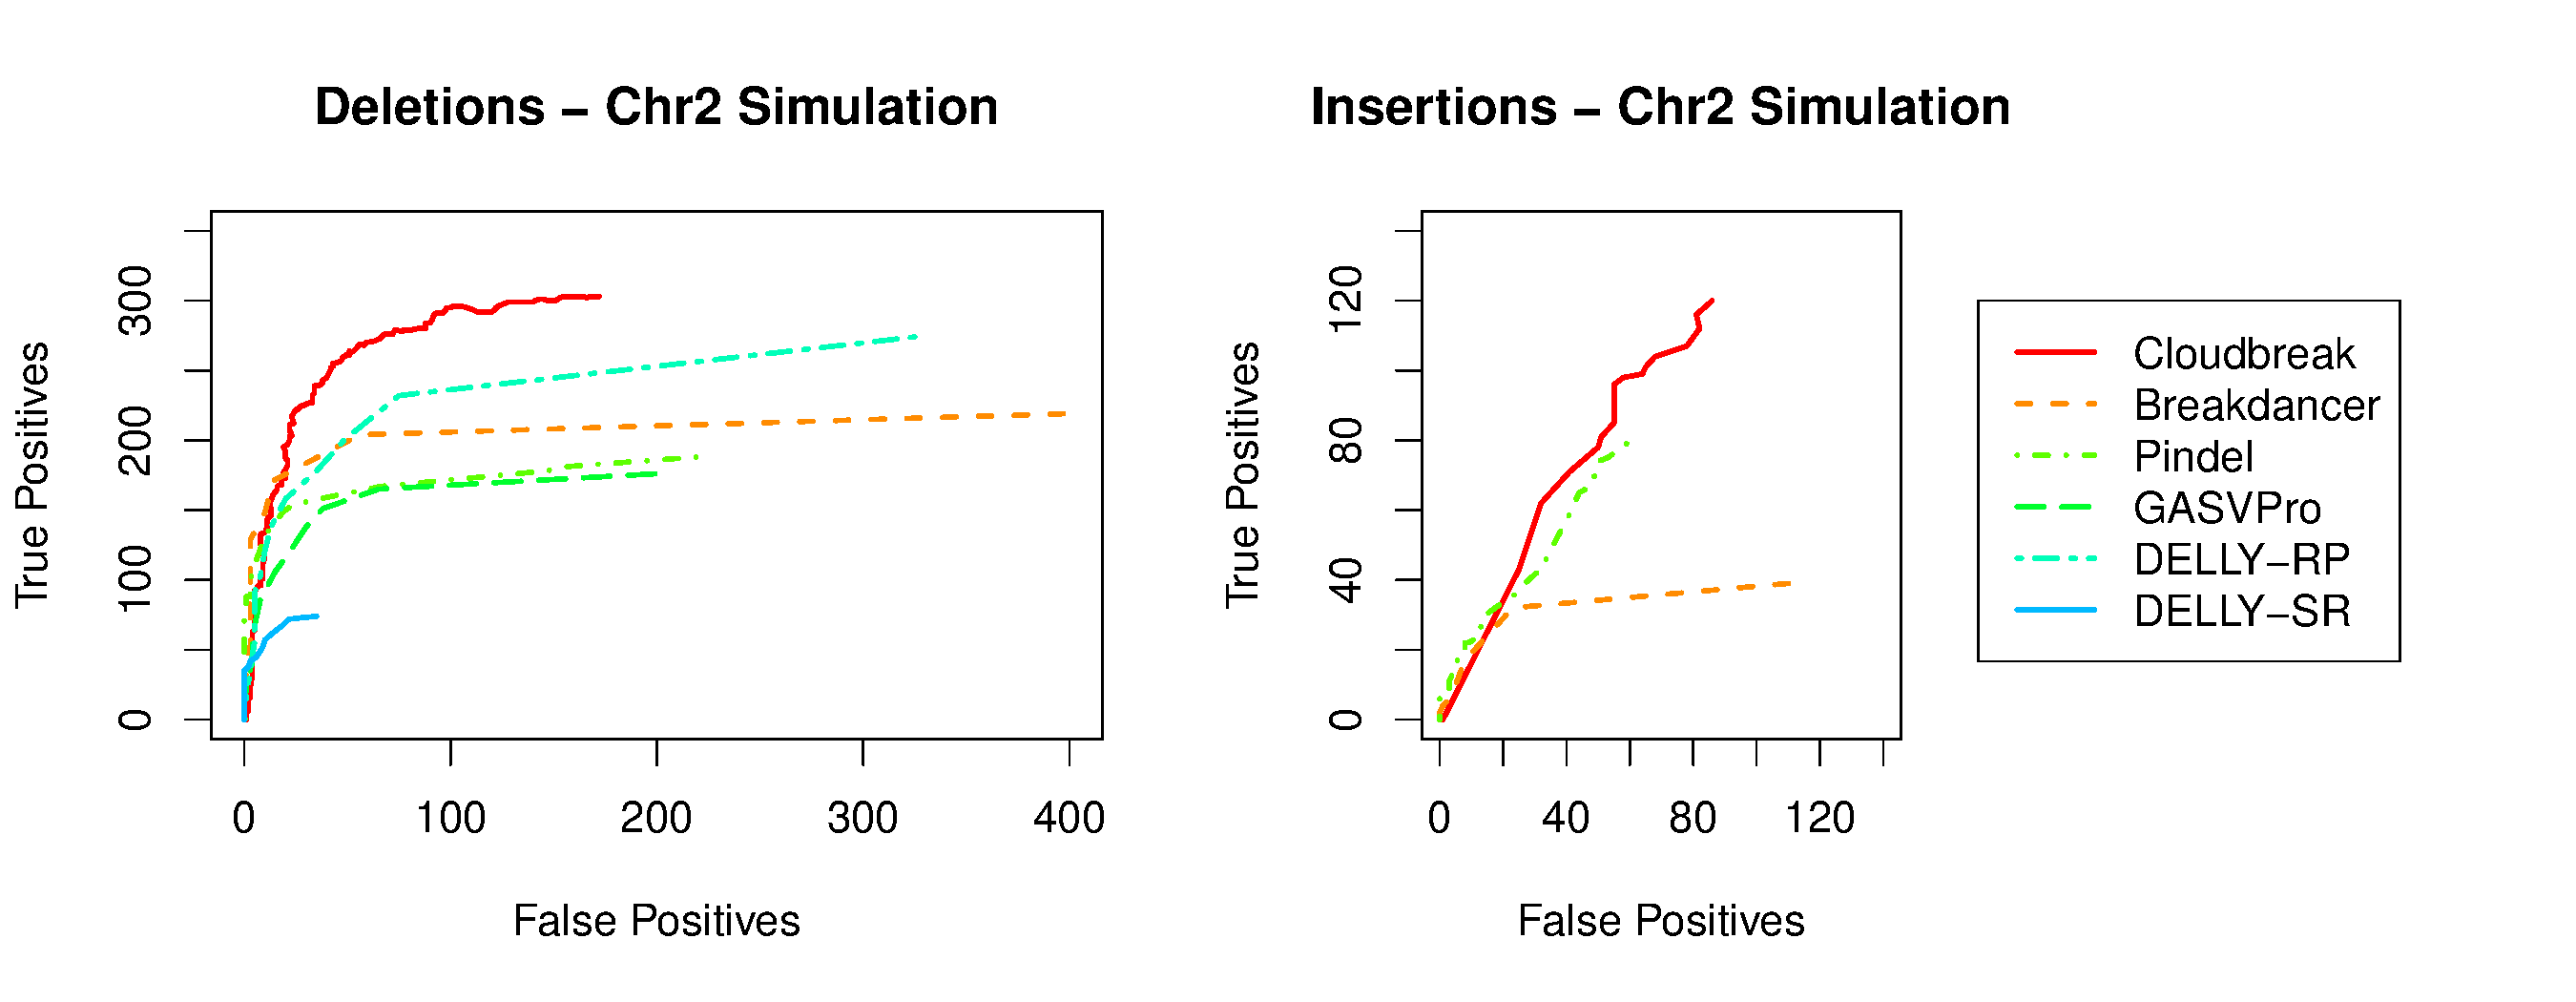
\includegraphics[width=1\textwidth]{figures/CHR2SIM_ROC_COMBINED_ROCS_POSTER.pdf}
\caption{Accuracy and runtime performance on a simulated data set. Receiver Operating Characteristic (ROC) curves showing the specificity and sensitivity of each tool to deletions and insertions larger than 40bp on a simulated set of reads giving diploid coverage of 30X on human chromosome 2. Deletions and insertions from the Venter genome were randomly added to one or both haplotypes. Each point on a curve represents a different threshold on the confidence of predictions made by that tool. Thresholds vary by: Cloudbreak - likelihood ratio; BreakDancer, DELLY, GASVPro - number of supporting read pairs; Pindel - simple score.}
\label{chr2CombinedRoc}
\end{figure}

Figure~\ref{chr2CombinedRoc} shows Receiver Operating Characteristics (ROC) curves of the performance of each algorithm for detecting deletions and insertions on the simulated data set. See Section~\ref{section_prediction_evaluation} for a description of how we identified correct predictions. All approaches show excellent specificity at high thresholds in this simulation. Cloudbreak provides the greatest specificity for deletions at higher levels of sensitivity, followed by DELLY. For insertions, Cloudbreak clearly provides the best combinations of sensitivity and specificity. Figure~\ref{chr2BestRuntimes} shows the runtimes for each tool on the simulated data set, parallelized when possible. Runtimes exlude alignment, which should be similar for all tools. Cloudbreak's runtime is half that of BreakDancer, the next fastest tool, processing the simulated data in under six minutes. Of course, Cloudbreak uses many more CPUs as a distributed algorithm. See Section~\ref{section_comparing_runtime} for a more detailed discussion of runtimes and the amount of parallelization that was done for each tool. The output which we obtained from MoDIL did not have a threshold that could be varied to correlate with the trade-off between precision and recall and therefore it is not included in ROC curves; in addition, MoDIL ran for 52,547 seconds using 250 CPUs in our cluster, so results are not included in the runtime figure. Apart from the alignment phase, which is embarrassingly parallel, the feature generation job is the most computationally intensive part of the Cloudbreak workflow. Therefore, to test the algorithm's scalability we measured the runtime of that job on Hadoop clusters made up of varying numbers of nodes and observed that linear speedups can be achieved in this portion of the algorithm by adding additional nodes to the cluster until a point of diminishing returns is reached (Figure~\ref{scalability}).

\begin{figure}
\centering
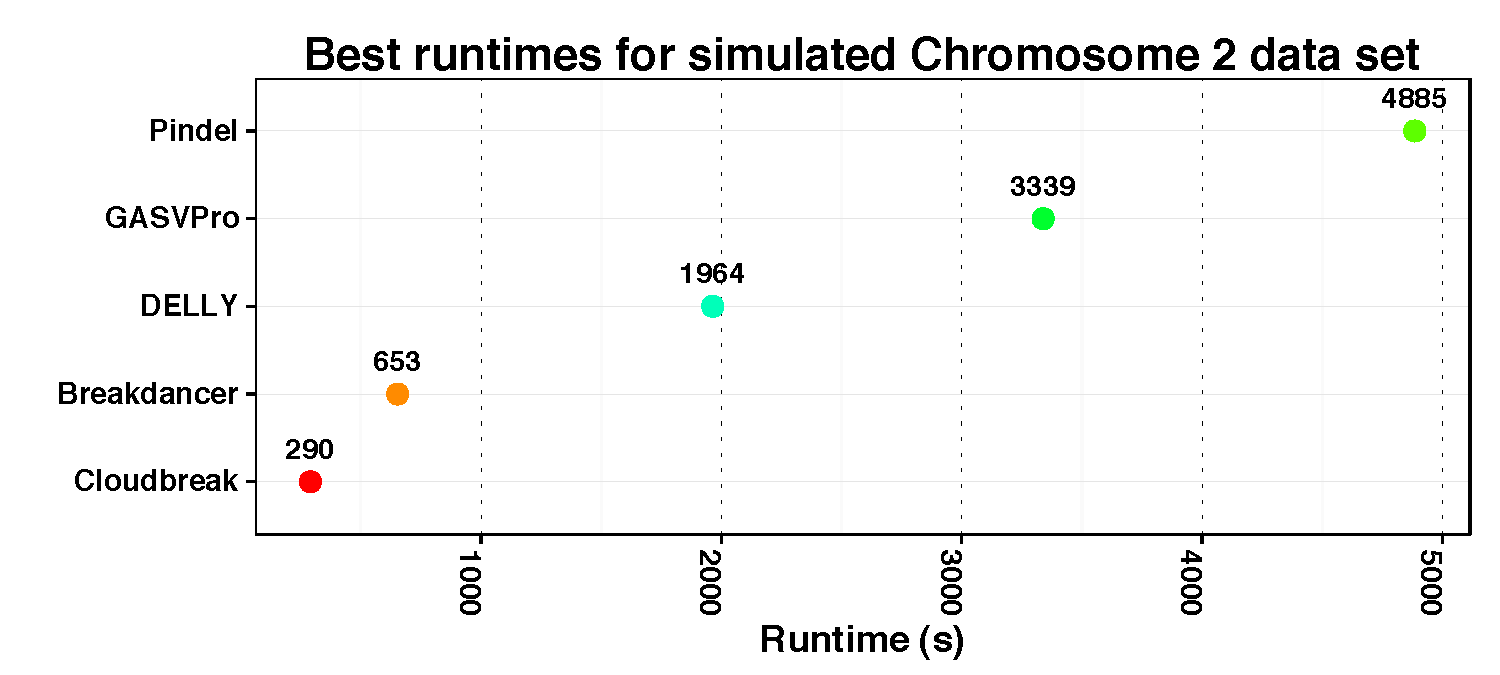
\includegraphics[width=1\textwidth]{figures/chr2BestRuntimes_horizontal.pdf}
\caption{Runtimes for each tool on the simulated data set, not including alignment time, parallelized when possible. See Section~\ref{section_comparing_runtime} for details on measuring and parallelizing the runtime of each tool.}
\label{chr2BestRuntimes}
\end{figure}

\begin{figure}
\centering
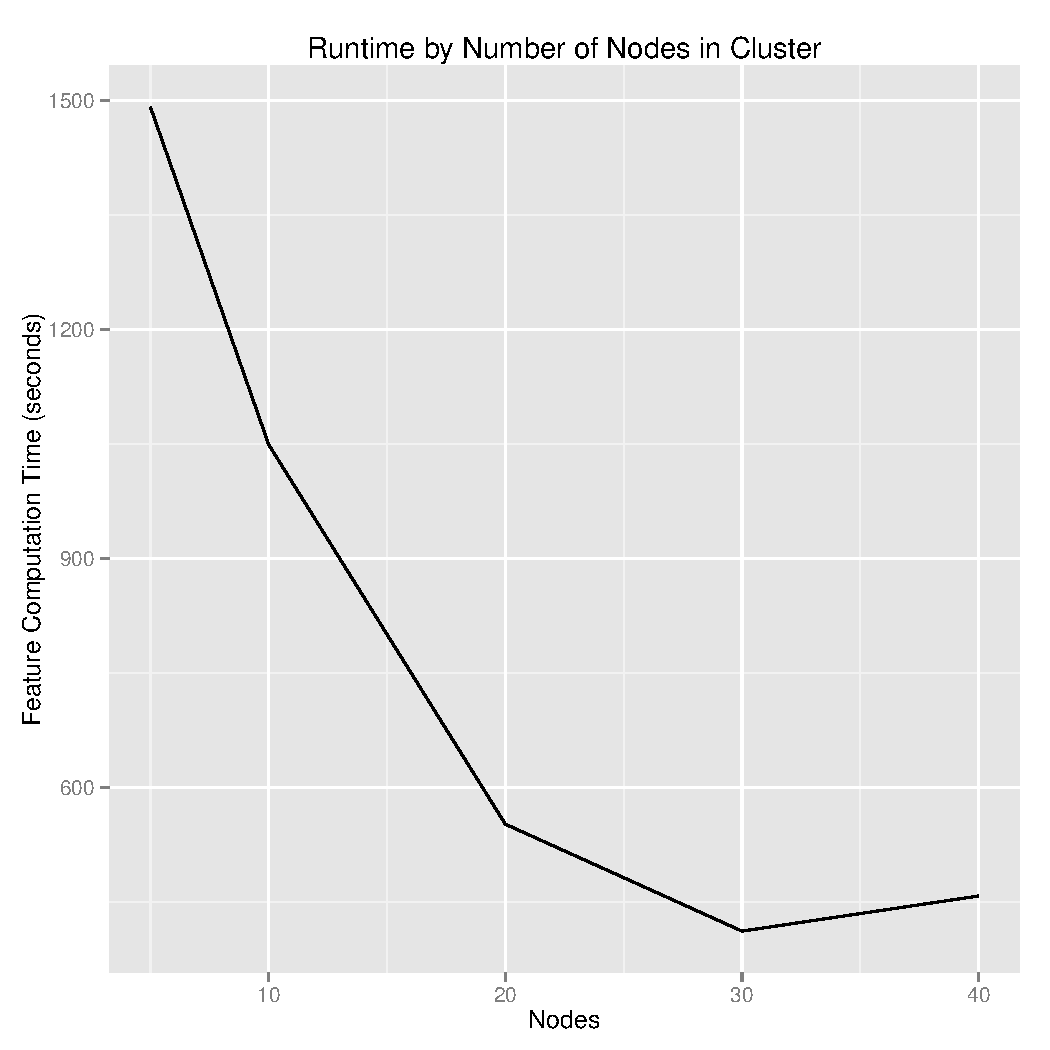
\includegraphics[width=.8\textwidth]{/Users/cwhelan/Documents/svpipeline/figures/runtimeByNodes.pdf}
\caption{Scalability of the Cloudbreak algorithm. Runtime of the Cloudbreak feature generation job for the simulated Chromosome 2 data is shown on Hadoop clusters consisting of varying numbers of compute nodes. Clusters were created in the Amazon Elastic Compute Cloud.}
\label{scalability}
\end{figure}

Choosing the correct operating point or threshold to set on the output of an SV calling algorithm can be difficult when operating on a new data set. The use of simulated data and ROC curves allows for some investigation of the performance characteristics of algorithms at varying levels. First, we characterized the predictions made by each algorithm at the operating point which gives them maximum sensitivity. For Cloudbreak we chose an operating point at which marginal improvements in sensitivity became very low. The results for both deletion and insertion predictions are summarized in Table~\ref{chr2DeletionAndInsertionPredsMaxSensitivity}. MoDIL and Cloudbreak exhibited the greatest recall for deletions. Cloudbreak has high precision and recall for deletions at this threshold, and discovers many more small deletions. For insertions, Cloudbreak has the highest recall, although recall is low for all four approaches. Cloudbreak again identifies the most small variants. Pindel is the only tool which can consistently identify large insertions, as insertions larger than the library insert size do not produce mapping signatures detectable by read-pair mapping. 

\begin{table}
\begin{center}
\resizebox{\textwidth}{!}{
\begin{tabular}{r|rrrr|rrrrr}
  \cline{2-10}
   &                     & Prec. & Recall & F1 & 40-100bp  & 101-250bp  & 251-500bp & 501-1000bp & $>$ 1000bp \\ 
\hline
\multirow{7}{*}{\begin{sideways}Deletions\end{sideways}} & Total Number &          &           &  &  224 &  84 & 82 &  31 & 26\\ 
  \hline
\cline{2-10}
&  Cloudbreak    &  0.638 & \textbf{0.678} & \textbf{0.657} & \textbf{153} (9)  & 61 (0) &  62 (0) & 12 (0) & 15 (0) \\ 
&  BreakDancer   &  0.356 & 0.49 & 0.412 & 89 (0)  & 54 (0) &  53 (0) & 8 (0) & 15 (0) \\ 
&  GASVPro        & 0.146 & 0.432 & 0.218 & 83 (2)  & 32 (0) &  55 (0) & 8 (0) & 15 (0) \\ 
&  DELLY-RP           & 0.457 & 0.613 & 0.613 & 114 (3)  & \textbf{68} (0) &  \textbf{66} (0) & 9 (1) & 17 (0) \\ 
&  DELLY-SR           & \textbf{0.679} & 0.166 &  0.266 & 0 (0)  & 3 (0) &  49 (0) & 6 (0) & 16 (0) \\ 
&  Pindel           & 0.462 & 0.421 &  0.44 & 96 (\textbf{11})  & 24 (0) &  48 (0) & 5 (0) & 15 (0)\\ 
&  MoDIL           & 0.132  & 0.66 & 0.22 & 123 (6)  & 66 (\textbf{3}) &  \textbf{66} (\textbf{11}) & \textbf{17} (\textbf{7}) & \textbf{23} (\textbf{8})\\ 
   \hline
\multirow{5}{*}{\begin{sideways}Insertions\end{sideways}} & Total Number &          &           & & 199 &  83 & 79 &  21 & 21\\ 
\cline{2-10}
&  Cloudbreak   &0.451 & \textbf{0.305}  & \textbf{0.364}  & \textbf{79} (\textbf{32})  & \textbf{32} (\textbf{18}) &  \textbf{11} (8) & 1 (0) & 0 (0) \\ 
&  BreakDancer & 0.262 & 0.0968  & 0.141  & 23 (5)  & 14 (5) &  2 (1) & 0 (0) & 0 (0) \\ 
&  Pindel          & \textbf{0.572} & 0.196 &  0.292 & 52 (25)  & 5 (1) &  10 (\textbf{9}) & \textbf{3} (\textbf{2}) & \textbf{9} (\textbf{9})\\ 
&  MoDIL          & 0.186 & 0.0521 &  0.0814 & 14 (1)  & 4 (0) &  1 (0) & 2 (\textbf{2}) & 0 (0)\\ 
\hline
\end{tabular}}
\end{center}
\caption{The number of simulated deletions and insertions in the 30X diploid chromosome 2 with Venter indels found by each tool at maximum sensitivity, as well as the number of those variants that were discovered exclusively by each tool (in parentheses). The total number of variants in each size class in the true set of deletions and insertions is shown in the first row of each section.}
\label{chr2DeletionAndInsertionPredsMaxSensitivity}
\end{table}

We also used the ROC curves to attempt to characterize the predictions made by each algorithm when a low false discovery rate is required. Table~\ref{chr2DeletionPredsFDR10} shows the total number of simulated deletions found by each tool when choosing a threshold that gives an FDR closest to 10\% based on the ROC curve. At this more stringent threshold, Cloudbreak identifies more deletions in every size category than any other tool. Performance on insertions never reached an FDR of 10\% for any threshold, so insertion predictions are not included in this table. 

\begin{table}
\begin{center}
\begin{tabular}{rrrrrr}
 \hline
 & 40-100bp & 101-250bp & 251-500bp & 501-1000bp & $>$ 1000bp \\ 
 Total Number & 224 & 84 & 82 & 31 & 26\\ 
 \hline
 Cloudbreak & \textbf{68} (17) & \textbf{67} (\textbf{10}) & \textbf{56} (\textbf{5}) & \textbf{11} (\textbf{3}) & \textbf{15} (\textbf{0}) \\ 
 BreakDancer & 52 (8) & 49 (2) & 49 (0) & 7 (0) & 14 (\textbf{0}) \\ 
 GASVPro  & 35 (2) & 26 (0) & 26 (0) & 2 (0) & 6 (\textbf{0}) \\ 
 DELLY-RP  & 22 (1) & 56 (1) & 40 (0) & 8 (0) & 12 (\textbf{0}) \\ 
 DELLY-SR  & 0 (0) & 2 (0) & 28 (0) & 2 (0) & 10 (\textbf{0}) \\ 
 Pindel  & 60 (\textbf{32}) & 16 (0) & 41 (2) & 1 (0) & 12 (\textbf{0})\\ 
 \hline
\end{tabular}
\end{center}
\caption{The number of simulated deletions in the 30X diploid chromosome 2 with Venter indels found by each tool at a 10\% FDR, as well as the number of those deletions that were discovered exclusively by each tool (in parentheses). The total number of deletions in each size class in the true set of deletions is shown in the second row of the header.}
\label{chr2DeletionPredsFDR10}
\end{table}

\subsection{Choice of Window Size}\label{section_window_size}

A key parameter choice for Cloudbreak is the size of the fixed-width, non-overlapping windows used for local feature computation. The experiments reported in this Chapter all used a window size of 25bp. Using the simulated data set, we evaluated the effect of choosing differing window sizes on runtime, breakpoint resolution, and accuracy. Figure~\ref{figure_runtime_by_window_size} shows the runtime of the feature computation and variant calling steps of Cloudbreak on the Chromosome 2 data set using differing window sizes. Runtime decreases dramatically with larger window sizes. For very small window sizes, the runtime is dominated by the variant extraction job, which is only parallelized by chromosome and therefore only runs on one core when running on the simulated data set. Table~\ref{chr2AccuracyByWindowSize} shows several accuracy measures for Cloudbreak running with varying window sizes, using the same threshold for each run. The greatest recall is achieved at very low window sizes, probably because evidence for smaller variants is less likely to be mixed in with non-variant supporting read pairs from the flanking regions. However, overall accuracy is high until window sizes reach 50bp, at which point recall decreases dramatically. Finally, we examined the effect of breakpoint accuracy on window size and found that it had little effect (Figure~\ref{breakpoint_resolution_by_windowSize}).

\begin{figure}
\centering
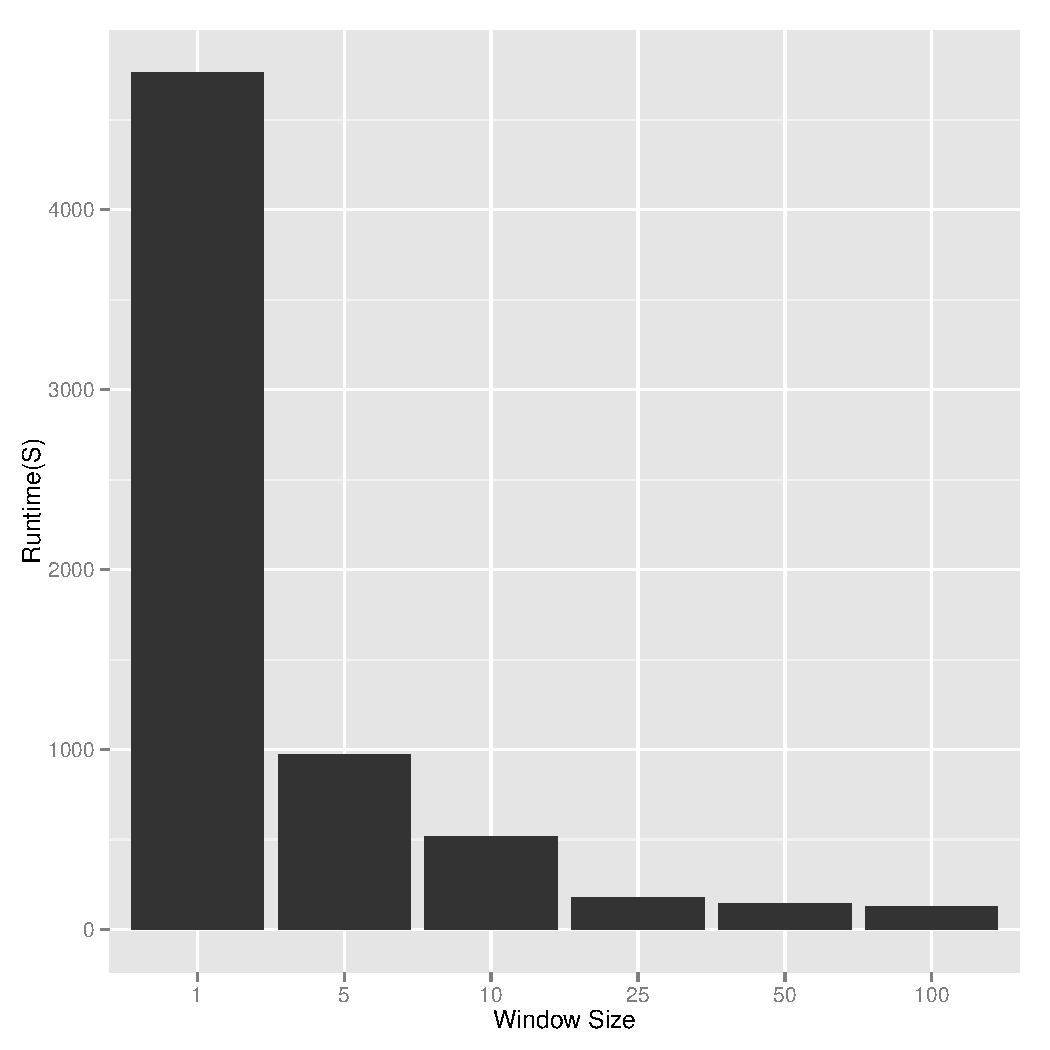
\includegraphics[width=.8\textwidth]{figures/runtime_by_windowSize.pdf}
\caption{Runtimes for Cloudbreak on the Chromosome 2 simulated data set using differing choices of window size. Runtimes include the feature computation and variant calling Cloudbreak Hadoop jobs.}
\label{figure_runtime_by_window_size}
\end{figure}

\begin{table}
\begin{center}
\begin{tabular}{r|rrrrr}
 \hline
 Window Size & Calls & True Positives & Precision & Recall & F1 \\ 
 \hline
   1 & 274 & 228 & 0.832 & 0.57 & 0.677 \\ 
   5 & 268 & 228 & 0.851 & 0.57 & 0.683 \\ 
   10 & 258 & 223 & 0.864 & 0.557 & 0.678 \\ 
   25 & 240 & 217 & 0.904 & 0.542 & 0.678 \\ 
   50 & 215 & 194 & 0.902 & 0.485 & 0.631 \\ 
   100 & 162 & 141 & 0.87 & 0.352 & 0.502 \\  
\end{tabular}
\end{center}
\caption{Accuracy measures for Cloudbreak on the Chromosome 2 simulated data set using different choices of window size. For each window size the same Cloudbreak score threshold was used (1.98).}
\label{chr2AccuracyByWindowSize}
\end{table}
\begin{figure}
\centering
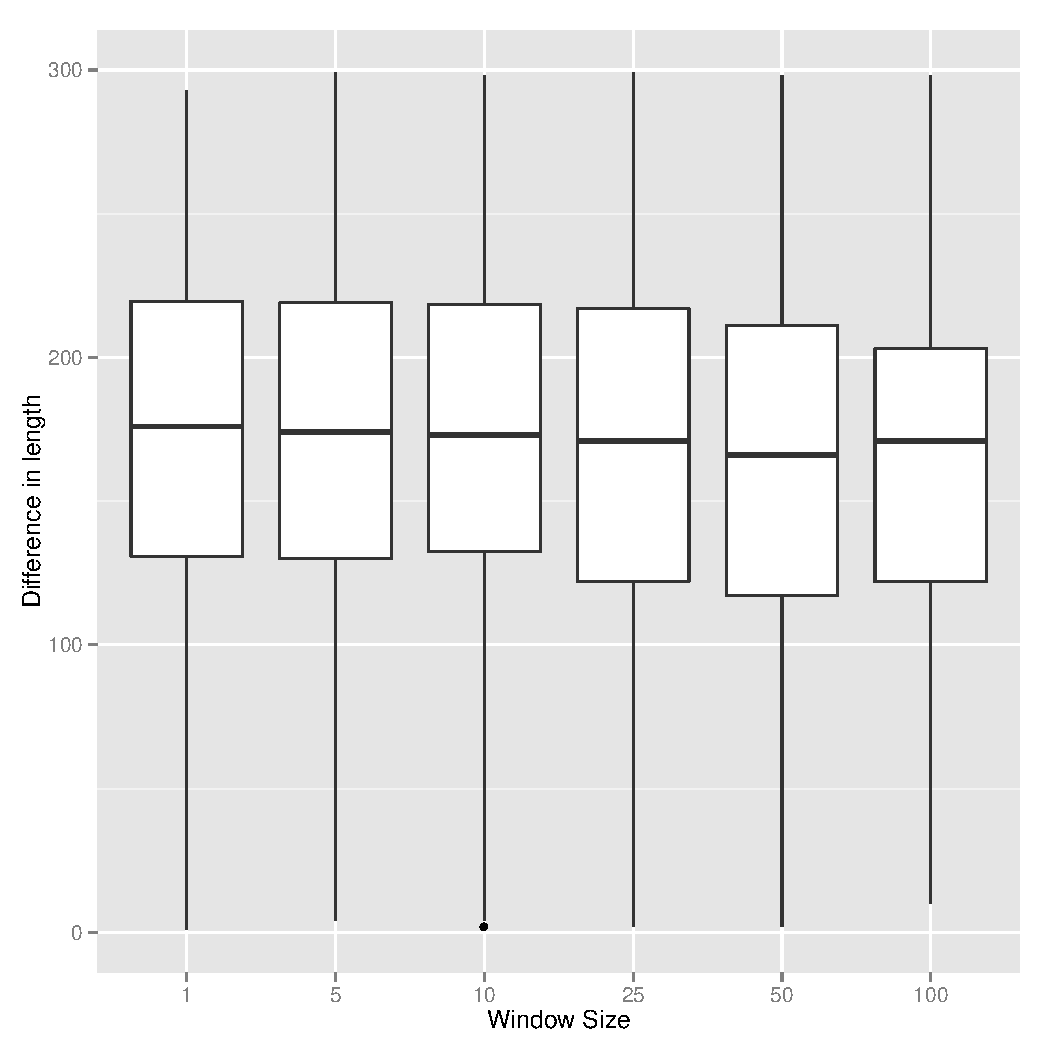
\includegraphics[width=.8\textwidth]{figures/breakpoint_resolution_by_windowSize.pdf}
\caption{Breakpoint resolution for Cloudbreak on the Chromosome 2 simulated data set using differing choices of window size.}
\label{breakpoint_resolution_by_windowSize}
\end{figure}

\section{Results on Biological Data}\label{section_na18507}

\subsection{Accuracy and Runtime}

\begin{figure}
\centering
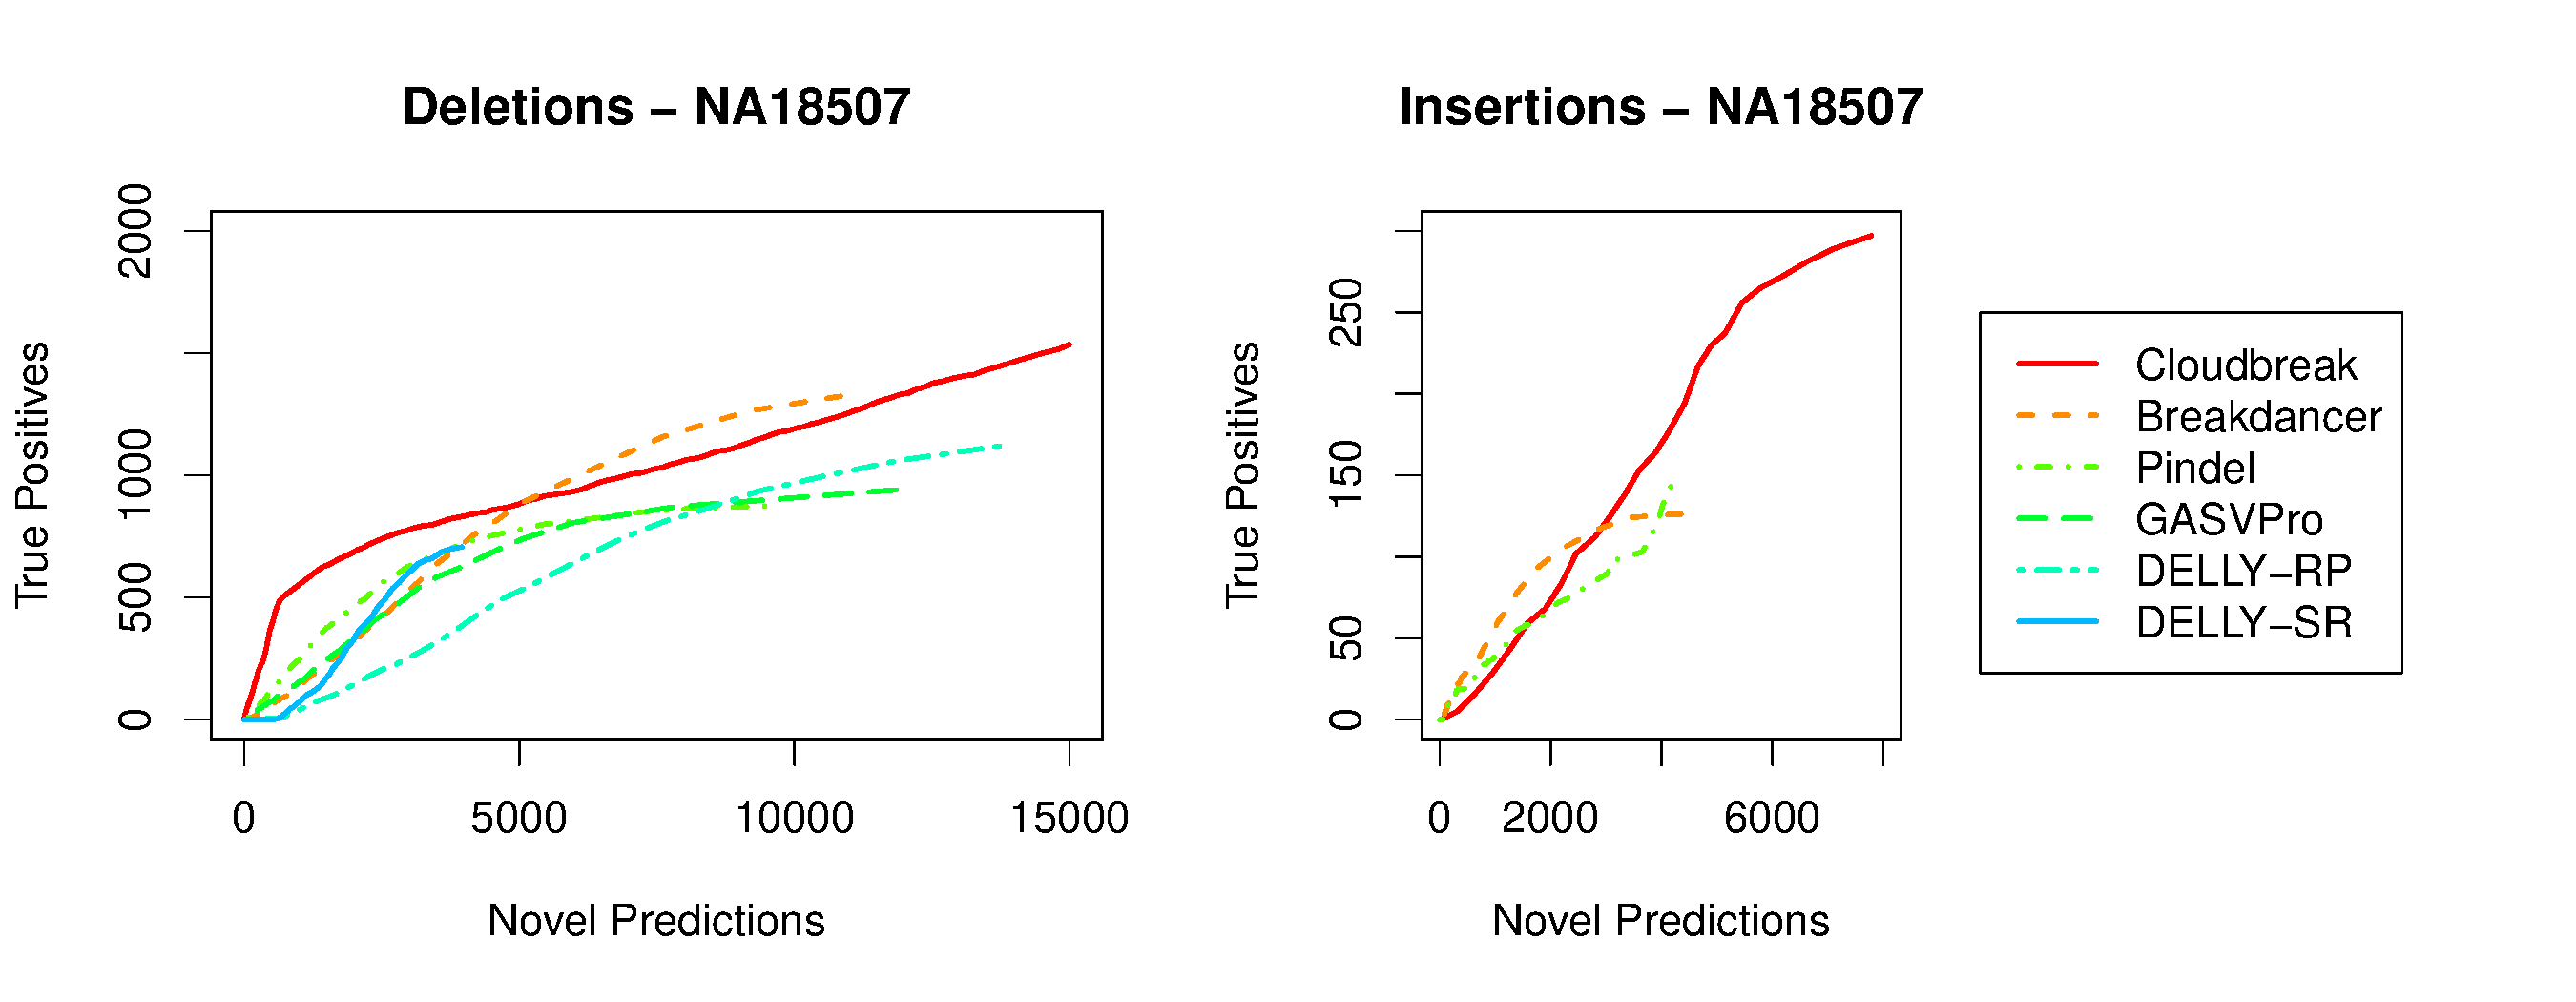
\includegraphics[width=1\textwidth]{figures/NA18507_COMBINED_ROCS_POSTER.pdf}
\caption{Accuracy on the 37X NA18507 sample. ROC curves for deletion and insertion prediction performance, tested against the combined gold standard sets of deletions taken from~\cite{Kidd:2008p926},~\cite{Mills:2011fi}, and~\cite{GenomesProjectConsortium:2012co}.}
\label{NA18507CombinedRoc}
\end{figure}

Figure~\ref{NA18507CombinedRoc} shows the performance of each algorithm on the NA18507 data set when compared against the gold standard set for both deletions and insertions. We were unable to run MoDIL on the whole-genome data set due to the estimated runtime and storage requirements. All other algorithms show far less specificity for the gold standard set than they did for the true variants in the single chromosome simulation, although it is difficult to tell how much of the difference is due to the added complexity of real data and a whole genome, and how much is due to missing variants in the gold standard set that are actually present in the sample. For deletions, Cloudbreak is the best performer at the most stringent thresholds, and has the highest or second highest precision at higher sensitivity levels. Cloudbreak has slightly lower accuracy for insertions than the other tools at more stringent thresholds, although it can identify the most variants at higher levels of sensitivity. Figure~\ref{NA18507BestRuntimes} and Table~\ref{runtimes} show the runtime of each of the tools on the NA18507 dataset. Cloudbreak processes the sample in under 15 minutes on our cluster, more than six times as fast as the next fastest program, BreakDancer, even when BreakDancer is run in parallel for each chromosome on different nodes in the cluster.

\begin{figure}
\centering
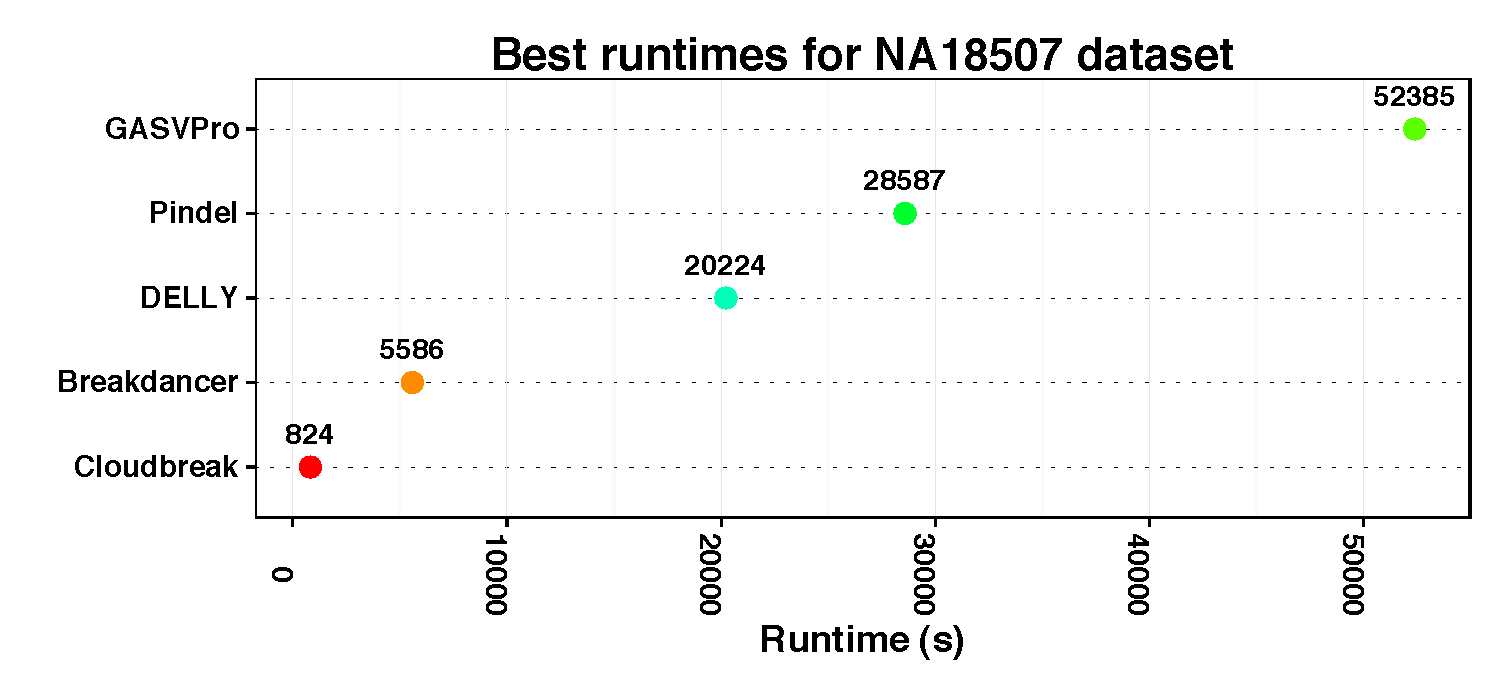
\includegraphics[width=1\textwidth]{figures/NA18507BestRuntimes_horizontal.pdf}
\caption{Runtimes for each tool on the NA18507 data set, not including alignment time, parallelized when possible. See Section~\ref{section_comparing_runtime} for details on measuring and parallelizing the runtime of each tool.}
\label{NA18507BestRuntimes}
\end{figure}

Given the high number of false positives produced by all tools at maximum sensitivity indicated by the ROC curves, we decided to characterize the predictions made by each tool at more stringent thresholds. We examined the deletion predictions made by each algorithm using the same cutoffs that yielded a 10\% FDR on the simulated chromosome 2 data set, adjusted proportionally for the difference in coverage from 30X to 37X. For insertions, again, we were forced to use the thresholds that gave maximum sensitivity for each tool due to the high observed FDR rates in the simulated data. The precision and recall at these thresholds with respect to the gold standard set, as well as the performance of each algorithm at predicting variants of each size class at those thresholds, is shown in Table~\ref{NA18507DeletionAndInsertionPreds}. For deletions, Cloudbreak has the greatest sensitivity of any tool at these thresholds, identifying the most variants in each size class. Pindel exhibits the highest precision with respect to the gold standard set. For insertions, Pindel again has the highest precision at maximum sensitivity, although according the ROC curve it is possible to choose a threshold for Cloudbreak with higher precision and recall. At maximum sensitivity, Cloudbreak identifies 120 more insertions from the gold standard set than Pindel, giving it by far the highest recall.

\begin{table}
\begin{center}
\resizebox{\textwidth}{!}{
\begin{tabular}{r|rrrr|rrrrr}
  \cline{2-10}
&  & Prec. & Recall & F1 & 40-100bp & 101-250bp & 251-500bp & 501-1000bp & $>$ 1000bp \\ 
\hline
\multirow{6}{*}{\begin{sideways}Deletions\end{sideways}} & Total Number & & & & 7,462 & 240 & 232 & 147 & 540 \\
  \hline
\cline{2-10}
& Cloudbreak & 0.0943 & \textbf{0.17} & 0.121 & \textbf{573} (\textbf{277})  & \textbf{176} (\textbf{30}) &  \textbf{197} (\textbf{18}) & \textbf{121} (\textbf{6}) & \textbf{399} (\textbf{24}) \\ 
& BreakDancer & 0.137 & 0.123 &  \textbf{0.13} & 261 (29)  & 136 (3) &  178 (0) & 114 (0) & 371 (0) \\  
&  GASVPro & 0.147 & 0.0474 &  0.0717 & 120 (21)  & 40 (2) &  85 (0) & 36 (0) & 128 (0) \\ 
&  DELLY-RP & 0.0931 & 0.1 &  0.0965 & 143 (6)  & 128 (3) &  167 (1) & 103 (0) & 323 (1) \\ 
&  DELLY-SR & 0.153 & 0.0485 &  0.0736 & 0 (0)  & 26 (0) &  123 (0) & 66 (0) & 203 (0) \\ 
&  Pindel & \textbf{0.179} & 0.0748 &  0.106 & 149 (8)  & 61 (0) &  149 (0) & 69 (1) & 217 (0) \\ 
\hline
\multirow{4}{*}{\begin{sideways}Insertions\end{sideways}} & Total Number & & & & 536 & 114 & 45 & 1 & 0 \\
\cline{2-10}
& Cloudbreak & 0.0323 & \textbf{0.455} &  0.0604 & \textbf{265} (\textbf{104})  & \textbf{49} (\textbf{24}) &  3 (1) & 0 (0)  & 0 (0)  \\ 
& BreakDancer & 0.0281 & 0.181 &  0.0487 & 97 (10)  & 27 (5) &  2 (1) & 0 (0) & 0 (0) \\  
&  Pindel & \textbf{0.0387} & 0.239 &  \textbf{0.0666} & 144 (45)  & 14 (7) &  \textbf{7} (\textbf{6}) & \textbf{1} (\textbf{1}) &  0 (0) \\ 
\hline
\end{tabular}}
\end{center}
\caption{The precision and recall with respect to the gold standard set of deletions and insertions for each tool on the NA18507 data, as well as the number of variants found in each size class found. Exclusive predictions are in parentheses. For deletions, the same cutoffs were used as for the simulated data as in Table~\ref{chr2DeletionPredsFDR10}, adjusted for the difference in coverage from 30X to 37X. For insertions, the maximum sensitivity cutoff was used.}
\label{NA18507DeletionAndInsertionPreds}
\end{table}

\subsection{Breakpoint Resolution}

We expected that the methods tested here would vary in their breakpoint resolution: SR methods can achieve single nucleotide breakpoint resolution, while RP methods depend on insert size evidence from overlapping fragments that will likely not indicate the exact location of the breakpoint. This distinction can be seen clearly in Figure~\ref{breakpoint_resolution}. Cloudbreak has the lowest resolution of any of the RP tools tested, with GASVPro also having relatively poor resolution. Pindel and DELLY-SR, meanwhile, use split read mappings to pinpoint the exact breakpoint correctly in many cases. Cloudbreak's resolution suffers because the independent calculation of features from the distribution of overlapping insert sizes does not allow the algorithm to keep track of the actual coordinates of the mapped reads from each pair, which other tools use to set bounds on the true breakpoint locations. Cloudbreak's goal, however, is to increase sensitivity and specificity to actual variants in the hopes that such calls could still be useful even if their resolution is limited. This seems reasonable to us, especially given the possibility of pipelines in which RP calls are validated \emph{in silico} by local assembly methods or split-read methods.

\begin{figure}
\centering
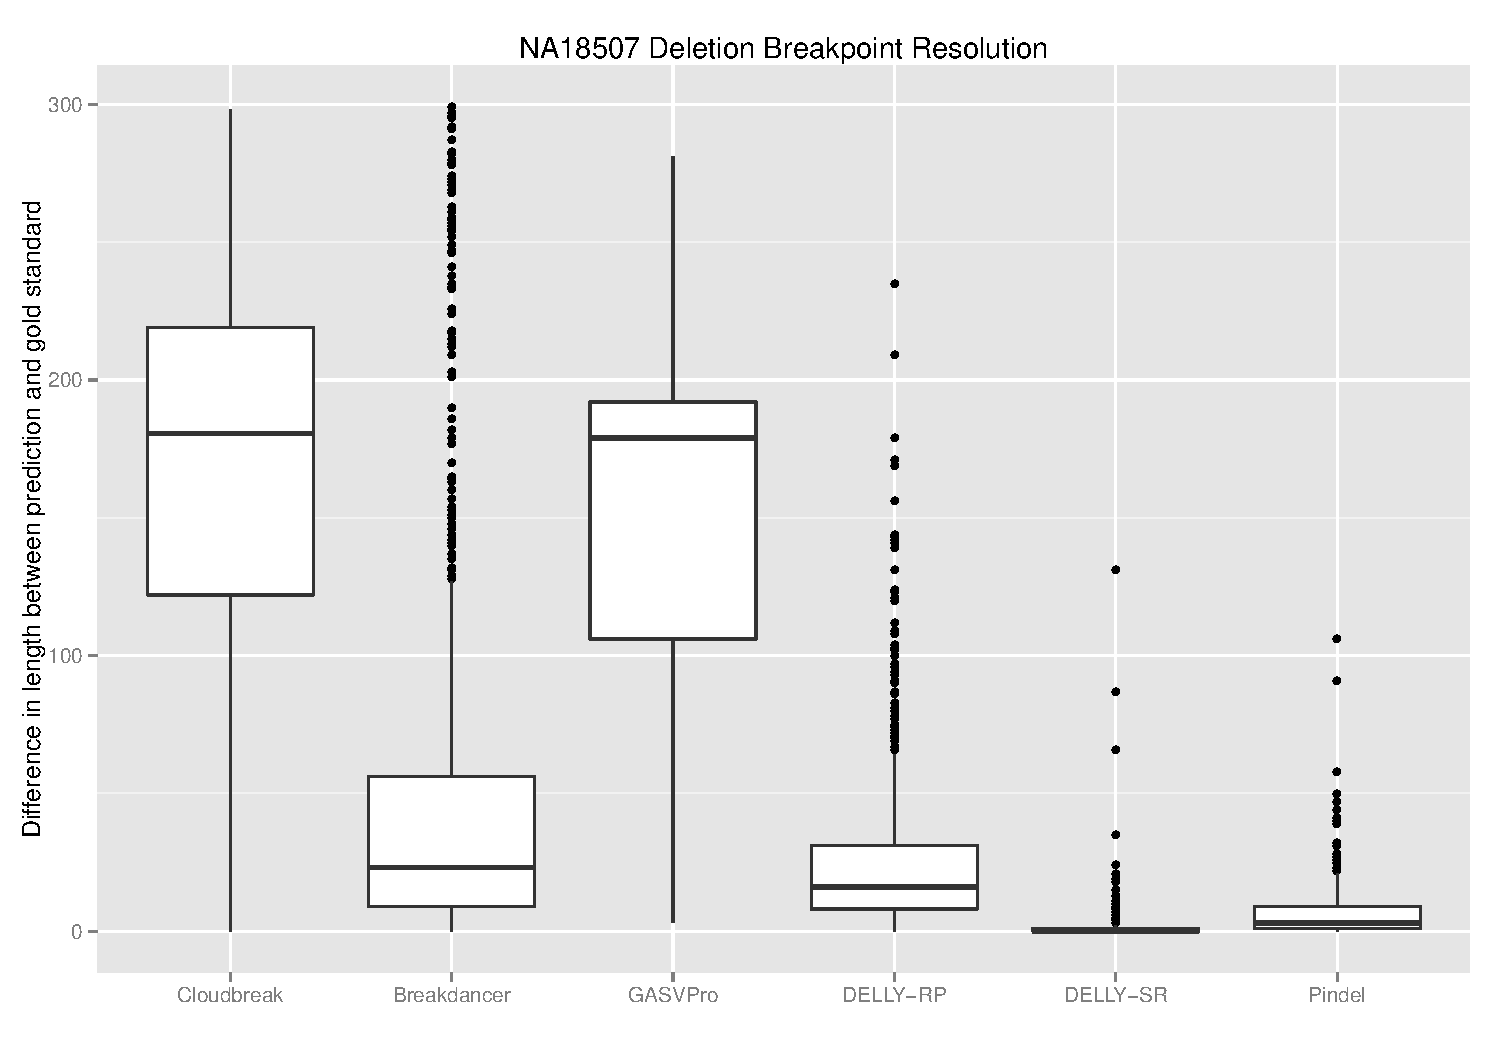
\includegraphics[width=.8\textwidth]{/Users/cwhelan/Documents/svpipeline/figures/breakpointResolutionNA18507.pdf}
\caption{Breakpoint resolution for each tool for deletions from the gold standard set on the NA18507 data. For each correctly predicted deletion, we calculated the difference in length between the true deletion and the prediction.}
\label{breakpoint_resolution}
\end{figure}

\section{Results on a Low-Coverage Cancer Data Set}\label{section_cloudbreak_eval_aml}

We also tested Cloudbreak on the sequencing data set obtained from a patient with acute myeloid leukemia (AML) described in Section~\ref{section_aml_pipeline}. This data set consisted of 76bp paired end reads with a mean insert size of 285bp and standard deviation of 50bp, yielding sequence coverage of 5X and physical coverage of 8X. Using a pipeline consisting of Novoalign, BreakDancer, and a set of custom scripts for filtering and annotating candidate SVs, we had previously identified a set of variants present in this sample and validated several using PCR, including 8 deletions. Cloudbreak was able to identify all 8 of the validated deletions, showing that it is still sensitive to variants even when using lower coverage data sets with a greater variance of insert sizes.

\section{Genotyping Variants}\label{section_genotyping_eval}

Because Cloudbreak explicitly models zygosity in its feature generation algorithm, it can predict the genotypes of identified variants. We tested this on both the simulated and NA18507 data sets. For the NA18507 data set, we considered the deletions from the 1000 Genomes Project, which had been genotyped using the population-scale SV detection algorithm Genome STRiP \cite{Handsaker:2011ki}. Cloudbreak was able to achieve 92.7\% and 95.9\% accuracy in predicting the genotype of the deletions it detected at our 10\% FDR threshold in the simulated and real data sets, respectively. Table~\ref{deletionGenotypeaccuracy} shows confusion matrices for the two samples using this classifier. None of the three input sets that made up the gold standard for NA18507 contained a sufficient number of insertions that met our size threshold and also had genotyping information. Of the 123 insertions detected by Cloudbreak on the simulated data set, 43 were heterozygous. Cloudbreak correctly classified 78 of the 80 homozygous insertions and 31 of the 43 heterozygous insertions, for an overall accuracy of 88.6\%.

\begin{table}
\begin{center}
\resizebox{\textwidth}{!}{
\begin{tabular}{r|r|rr|rr|}
\multicolumn{2}{c}{}  & \multicolumn{4}{c}{Actual Genotypes} \\
\multicolumn{2}{c}{}  & \multicolumn{2}{c}{Simulated Data} & \multicolumn{2}{c}{NA18507} \\
\cline{3-6}
\multicolumn{2}{c|}{} &  Homozygous & Heterozygous & Homozygous & Heterozygous \\ 
\cline{2-6}
\multirow{2}{*}{\shortstack{Predicted \\ Genotypes}} & Homozygous & 35 & 2 &  96 & 21 \\
 & Heterozygous & 0 & 39 &  2 & 448 \\
\cline{2-6}
\end{tabular}
}
\end{center}
\caption{Confusion matrices for the predicted genotype of deletions found by Cloudbreak on both the simulated and NA18507 data sets.}
\label{deletionGenotypeaccuracy}
\end{table}

\section{Notes on Evaluating  Runtime}\label{section_comparing_runtime}

We implemented and executed Cloudbreak on a 56-node Hadoop cluster, with 636 map slots and 477 reduce slots. Not including alignment time, we were able to process the Chromosome 2 simulated data in under six minutes, and the the NA18507 data set in under 15 minutes. For the simulated data set we used 100 reducers for the compute SV features job; for the real data set we used 300. The bulk of Cloudbreak's execution is spent in the feature generation step. Extracting deletion and insertion calls take under two minutes each for both the real and simulated data sets; the times are equal because each reducer is responsible for processing a single chromosome, and so the runtime is bounded by the length of time it takes to process the largest chromosome. 

Cloudbreak's elapsed times are faster than all of the other tools tested; however, there are several ways in which to compare runtime performance between tools that support different levels of parallelization. In Table \ref{runtimes} we display a comparison of runtimes on the real and simulated data sets for all of the tools evaluated in this work. We report runtimes for each tools run in its default single-threaded mode, as well as for levels of parallelization achievable with basic scripting, noting that one of the key advantages of Hadoop/MapReduce is the ability to scale parallel execution to the size of the available compute cluster without any custom programming. Pindel allows multi-threaded operation on multicore servers. Pindel and BreakDancer allow processing of a single chromosome in one process, so it is possible to execute all chromosomes in parallel on a cluster that has a job scheduler and shared filesystem. BreakDancer has an additional preprocessing step (\texttt{bam2cfg.pl}) which runs in a single thread. DELLY suggests splitting the input BAM file by chromosome, after which a separate DELLY process can be executed on the data for each chromosome; splitting a large BAM file is a time consuming process and consumes most of the time in this parallel workflow, in fact making it faster to run in single-threaded mode. GASVPro allows parallelization of the MCMC component for resolving ambiguously mapped read pairs; however, this requires a significant amount of custom scripting, and we did not find that the MCMC module consumed most of the runtime in our experiments, so we do not attempt to parallelize this component. The MoDIL distribution contains a set of scripts that can be used to submit parallel jobs to the SGE scheduling engine or modified for other schedulers; we adapted these for use in our cluster.

\begin{table}
\begin{center}
\resizebox{\textwidth}{!}{
\begin{tabular}{r|r|rrr|rrr}
\multicolumn{2}{c}{}  & \multicolumn{3}{c}{Simulated Data} & \multicolumn{3}{c}{NA18507} \\
\hline
 & SV Types &  Single CPU & Parallel & Proc. &  Single CPU & Parallel & Proc.  \\ 
  \hline
  Cloudbreak & D,I &   NA    & 290 & 312    & NA         & 824 & 636 \\ 
  BreakDancer & D,I,V,T &  653   & NA       & NA          & 134,170 &  5,586 & 84 \\
  GASVPro & D,V   &  3,339  & NA       & NA         & 52,385  & NA & NA \\
  DELLY & D         &  1,964 & NA          & NA      & 30,311  & 20,224 & 84 \\
  Pindel & D,I,V,P         & 37,006 &  4,885     & 8          &  284,932  & 28,587 & 84 \\ 
  MoDIL & D,I        &  NA      & 52,547 & 250 & NA         & NA  & NA\\ 
   \hline
\end{tabular}
}
\end{center}
\caption{Runtimes (elapsed) on both data sets of each tool tested, in single-processor and parallel mode. For parallel runs, Proc. is the maximum number of simultaneously running processes or threads. All times are in seconds. The types of variants detected by each program are listed with the abbreviations: D - deletion; I - insertion; V - Inversion; P - duplication; T - translocation. Interchromosomal translocations are only detected by BreakDancer in single CPU mode. }
\label{runtimes}
\end{table}

In parallel execution, the total time to execute is bounded by the runtime of the longest-running process. In the case of chromosome-parallelizable tools including BreakDancer, Pindel, and DELLY, this is typically the process working on the largest chromosome.\footnote{We note that one BreakDancer process, handling an unplaced contig in the hg19 reference genome, never completed in our runs and had to be killed manually; we exclude that process from our results.} In the case of MoDIL's run on the simulated data, we found that the different processes varied widely in their execution times, likely caused by regions of high coverage or with many ambiguously mapped reads. Cloudbreak mitigates this problem during the time-consuming feature generation process by using Hadoop partitioners to randomly assign each genomic location to one of the set of reducers, ensuring that the work is evenly distributed across all processes. This distribution of processing across the entire cluster also serves to protect against server slowdowns and hardware failures - for example, we were still able to complete processing of the NA18507 data set during a run where one of the compute nodes was rebooted midway through the feature generation job.

\section{Choice of Aligner and Use of Multiple Mappings}\label{section_multiple_mappings_eval}

\begin{figure}
\centering
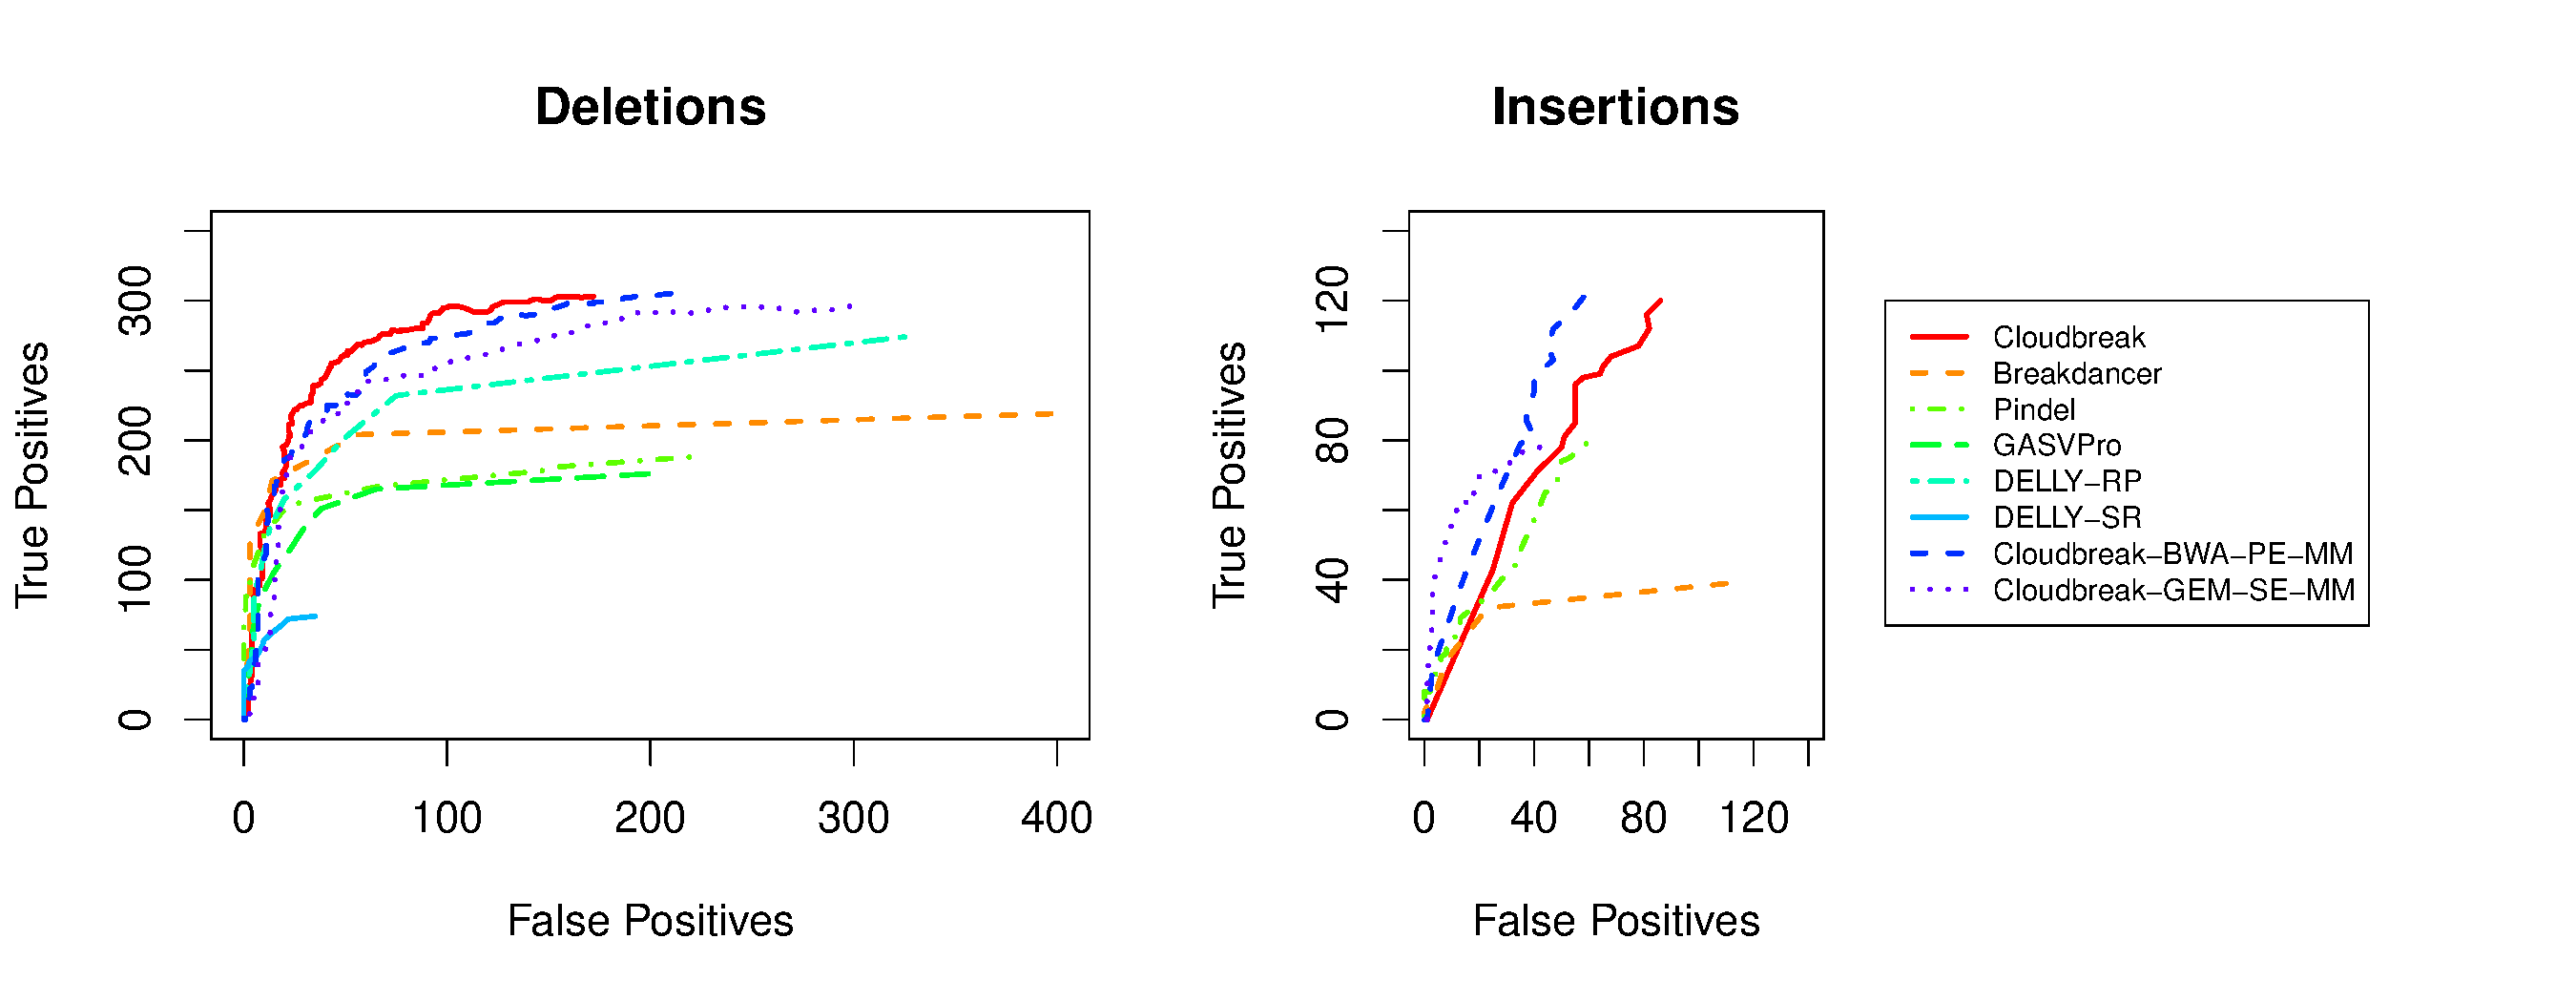
\includegraphics[width=1\textwidth]{/Users/cwhelan/Documents/svpipeline/figures/CHR2SIM_ROCS_MULTIPLE_MAPPINGS.pdf}
\caption{Cloudbreak performance on the chromosome 2 simulation using different alignment strategies. ROC curves show the number of true positives and false positives for each operating point for deletions and insertions. The Cloudbreak alignment strategies are: 1) ``Cloudbreak'': Alignments generated with BWA in paired-end mode, reporting the best hit for each pair. 2) ``Cloudbreak-BWA-PE-MM'': Alignments generated with BWA in paired-end mode, reporting up to 25 additional hits for each mapping. 3) ``Cloudbreak-GEM-SE-MM'': Alignments generated by running the GEM aligner in single-ended mode, reporting up to 1000 additional hits per alignment. Considering multiple mappings improves Cloudbreak's specificity for insertions but decreases sensitivity to deletions.}
\label{alignment_comparison}
\end{figure}

As mentioned in Section~\ref{section_incorrect_and_ambiguous_mappings}, one goal for developing Cloudbreak was to see if the use of Hadoop would allow productive use of large sets of possible mappings for ambiguously mapped read pairs. Therefore, we also tested the effect of using different aligners and including multiple mappings for ambiguously mapped reads. In addition to the BWA paired end best alignments used in the results reported above, we also used BWA in paired end mode set to report up to 25 possible mapping locations for each ambiguously mapped read pair, as well as the GEM aligner run in single ended mode on each read in each pair and set to report up to 1000 additional mappings per read. Interestingly, we found that including multiple mappings increases accuracy on insertions, but decreases performance for deletions (Figure~\ref{alignment_comparison}). This seems to indicate that while BWA's paired end mode is very good at picking correct alignments for pairs that map with long implied insert sizes, it seems to not be as good at finding correct pairings for the shorter distances indicative of insertions. We also examined the ability of all of the approaches, including Cloudbreak using both the BWA unambiguous best alignments and the GEM alignments, to detect events in repetitive regions of the genome, as shown in Table~\ref{predsByRepmask}. We found that all of the tested methods detected a similar proportion of such variants, although we did find that when used with the GEM multiple mappings, Cloudbreak does exclusively find a set of both deletion and insertion variants. In terms of runtime, use of the large set of multiple mappings did not change elapsed time to run the simulated data sample greatly, taking 308 seconds versus the 290 sections reported in the previous section. For the NA18507 dataset, the difference in runtime was more substantial, with Cloudbreak moving from taking 824 seconds to process the best alignments to 2,310 seconds to process the multiple mappings data set, a runtime which is still almost 50\% less than the next fastest approach, BreakDancer parallelized by chromosome. Although the runtimes were very manageable, we see no substantial benefit in terms of accuracy in using large sets of ambiguous mappings, at least in our current implementation.

\begin{table}
\begin{center}
\begin{tabular}{r|r|rr|rr}
  \cline{2-6}
 & & \multicolumn{2}{c}{Simulated Data} & \multicolumn{2}{c}{NA18507} \\
\hline
 & & Non-repeat & Repeat  & Non-repeat & Repeat \\ 
\multirow{9}{*}{\begin{sideways}Deletions\end{sideways}} & Total Number & 120 & 327 & 562 & 8059 \\ 
  \cline{2-6}
&  Cloudbreak  & 62 (0) & \textbf{241} (3) & \textbf{300} (\textbf{44}) & \textbf{1166} (\textbf{150}) \\ 
&  Cloudbreak-GEM  & 65 (2) & 230 (4) & 226 (8) & 1001 (17) \\ 
&  BreakDancer & 42 (0) & 177 (0) & 192 (11) & 868 (20) \\
&  GASVPro     & 37 (1) & 156 (1) & 79 (6) & 330 (16) \\
&  DELLY-RP       & 57 (1) & 217 (2) & 152 (4) & 712 (3) \\
&  DELLY-SR       & 3 (0) & 71 (0) & 27 (0) & 391 (0) \\
&  Pindel      & 26 (4) & 162 (7) & 109 (2) & 536 (6) \\ 
&  MoDIL      & \textbf{72} (\textbf{12}) & 223 (\textbf{16}) & NA & NA \\ 
   \hline
\multirow{6}{*}{\begin{sideways}Insertions\end{sideways}} & Total Number & 133 & 270 & 341 & 355 \\ 
\cline{2-6}
&  Cloudbreak  & \textbf{32} (7) & \textbf{91} (\textbf{30}) & \textbf{169} (\textbf{41}) & \textbf{148} (\textbf{43}) \\ 
&  Cloudbreak-GEM  & 21 (0) & 58 (7) & 137 (30) & 135 (32) \\ 
&  Breakdancer & 17 (5) & 22 (3) & 82 (22) & 44 (8) \\
&  Pindel      & 25 (\textbf{16}) & 54 (26) & 84 (13) & 82 (15) \\ 
&  MoDIL      & 5 (0) & 16 (2) & NA & NA \\ 
\hline
\end{tabular}
\end{center}
\caption{Detected deletions and insertions on the simulated and NA18507 data sets identified by each tool, broken down by whether the deletion overlaps with a RepeatMasker-annotated element. For all calls the maximum sensitivity cutoff was used.}
\label{predsByRepmask}
\end{table}

\section{Discussion}

We have demonstrated the Cloudbreak can deliver excellent accuracy at identifying regions that contain deletion and insertion SVs while at the same time achieving dramatically faster runtimes than other approaches through the use of the Hadoop framework and its implementation of parallel computing with data locality. In particular, the algorithm we developed for Cloudbreak is better able to identify small variants (50bp-150bp) than other tools. The downside to Cloudbreak's performance on our evaluations is its poor breakpoint resolution. As we mentioned previously, we believe that in most cases, predictions from SV detection tools require further validation, either through wet lab techniques or by further computational validation through techniques such as the split-read refinement offered by tools like DELLY, or through breakpoint assembly techniques such as TIGRA~\cite{Chen:2013gf}. In the next chapter, we will demonstrate an additional technique that improves Cloudbreak's resolution: a discriminative machine learning framework that can identify breakpoint locations by integrating read pairing, depth of coverage, and split read signals from sequencing data sets.

\chapter{Extending Local Feature Based Models of SV Detection in a Discriminative Machine Learning Framework}\label{chap_crf}

In my formulation of a general approach for SV prediction in the MapReduce framework, a crucial phase is the computation of a set of features for each genomic location. In my current implementation of Cloudbreak, these features are the parameters which are estimated by fitting a GMM to the distribution of insert sizes that span that location. However, the nature of these features are purposefully not specified in the algorithmic framework to allow flexibility in the implementation of the framework.

Given a set of arbitrary features that encode information about a set of loci that are connected in a sequence, a natural approach is to apply techniques from machine learning to identify regions of interest in that sequence, rather than the heuristics and noise reduction techniques from signal processing that are used in the Cloudbreak implementation described in Chapter \ref{chap_cloudbreak_impl}. Discriminative machine learning techniques have been applied to SV detection in the packages forestSV~\cite{Michaelson:2012fj} and SVM$^2$~\cite{Chiara:2012ey}. However, neither of these tools use machine learning techniques that take into account the sequential nature of the data. 

\section{SV Detection as a Sequence Labeling Problem}

In the the algorithmic framework for solving the structural variation detection problem in MapReduce that we presented in Chapter \ref{chap_framework}, we reduced the problem to one of computing a set of features that described the short read evidence for SVs at each of a set of small regions along the genome. These are then transformed into variant calls by a function which examines the features along each chromosome of the reference sequentially and identifies contiguous blocks of regions with features values that combine to coherently indicate the presence of a variant. This latter part of the process, which we named the \textsc{Postprocess} function in Algorithm \ref{cb_algo}, can be thought of as a sequencing labeling problem based on sequence features. To take the example of deletion detection, we could define two labels: ``Deletion'' if the window participates in a deletion variant, and ``No Deletion'' if it does not. More formally, we can let $Y_i$ be the label at genomic window $i$, where $1 \le i \le n$ where $n$ is the number of windows in the chromosome. If we similarly name the features for genomic window $i$ $X_i$, we can then refer to the entire sequence of labels and features as $Y$ and $X$, respectively.

The goal of fhe \textsc{Postprocess} function, can be broken down into two parts: first, to assign a label to each window in the reference sequence, and second, to consolidate neighboring windows with the same label into variant calls which affect larger regions. Using this model to think about the implementation of Cloudbreak described in Chapter \ref{chap_cloudbreak_impl}, we used a simple linear threshold on the likelihood ratio of the insert size data to label each window, and then consolidated neighboring windows with hand-tuned rules such as the median filter and restriction on the estimated mean of the second GMM component. These latter rules were made necessary by the noisy nature of the data and the simplicity of the window-labeling procedure. However, if we had a completely accurate window-labeling procedure, we could remove much of the complexity of the consolidation step. Since real world data is noisy, however, the best that we can do is to try to find the most likely sequence of labels given the observed data:

\[ \argmax_Y P(Y|X) \]

To acheive the goal of a more principled and more accurate window-labeling procedure we would need to be able to take into account information from multiple features, as well as the labels of nearby windows. In other words, the label of each window should be dependent not only on the observed features at that window but also on the labels of other windows nearby. Probabilistic graphical models provide a framework for defining and learning models that describe these types of dependencies. \todo{Describe PGMs here} One class of graphical model that has been used extensively for sequence labeling tasks in bioinformatics are Hidden Markov Models (HMMs). \todo{describe HMMs}

\section{Integrating Features with Conditional Random Fields}

To overcome these drawbacks of HMMs, we implemented a linear-chain conditional random field~\cite{Lafferty:2001:CRF:645530.655813} model to label genomic deletions. The model was developed using Factorie~\cite{mccallum09:factorie}. Factorie is a toolkit written in Scala that supports a wide variety of factor-graph based models, trainers, and tools, particularly for NLP tasks such as named entity recognition. Our Factorie-based implementation of a structural variation detection program consists of two parts: a modular and configurable set of code for data management of features defined along the genome, along with conversion of real-valued features into into binary binned feature values, and code to construct, train, and run inference on linear-chain CRF models. The code developed for this project was written in Scala and is available on GitHub at \url{http://github.com/cwhelan/svfactorie}. 

\todo{Feature management. Integration of disparate tracks. Selection of windows. Cumulative vs discrete binning.}

\todo{Model training}

We developed a linear chain CRF model in Factorie. For optimization during training we use the LGBFS algorithm with L2 regularization. We have also experimented with other optimizers including the online AdaGrad regularized dual averaging algorithm \cite{Duchi:2011:ASM:1953048.2021068} with L1 regularization but did not see large differences in preliminary testing. To conduct inference we use the Viterbi max-product belief propogation algorithm.

\section{Features for SV Detection}

As described in Chapter \ref{chap_background}, there are three main signals available for SV detection in short read sequencing data sets: those that come from read pairing information, those that come from read depth, and those that come from split reads. The creation of a discriminative machine learning framework as described above can be used with any arbitrary set of features. Therefore it is possible to create feature sets that combine information from all three SV detection signals and integrate them into this framework. In addition, we can model interactions between features and use those in our predictions. Finally, the arbitrary nature of the feature function allows us to incorporate prior knowledge about given genomic regions, including sequence annotations. We have constructed a feature set that includes all of these types of features, as described below:

\subsection{Read Pair Features}

Read pair features are those that are based upon the inferred insert sizes and orientations linking paired reads, as described previously. We use the following RP features:

\begin{itemize}

\item The three features generated by Cloudbreak and described in Chapter~\ref{chap_cloudbreak_impl}: the log likelihood ratio of the insert sizes observed at each window in the two-component GMM fit vs. the likelihood under the expected normal distribution for the sample; the estimated mean $\mu_2$ of the second component of the two-component GMM, and $\alpha$, the estimated weight of the second component in the two-component GMM.

\item Insert size change point features: in addition to the insert size calculations described in the Cloudbreak implementation, we also wanted to consider alternative features based on insert sizes. In particular, we wanted to test whether the addition of features that indicate whether a window represents a point at which the insert size distribution in a local surrounding region is changing would improve identification of variants. We compute such a score as follows: let $i$ be the index of a window in the genome, and $S_{i..j}$ be the list of observed insert sizes spanning the windows labeled $i$ through $j$. Now consider a local neighborhood of size $n$ which comprises the windows $i-\frac{n}{2},...,i,...,i+\frac{n}{2}$. Let $\Theta_{i..j}$ be model parameters that can be estimated from the distribution of insert sizes $S_{i..j}$, and $P(S_{i..j}|\Theta_{i..j})$ be the likelihood of observing $S_{i..j}$ under the model with parameters $\Theta$. We can calculate a change score for each window $i$ by examining the likelihood of the data in the halves of the neighborhood to the right and left of that window, by estimating $P(S_{i-\frac{n}{2}..i})$ and $P(S_{i+1..i+\frac{n}{2}})$. Simultaenously, we can perform the same estimates for all of the data in the neighborhood and compute $P(S_{i-\frac{n}{2}..i+\frac{n}{2}})$. The likelihood ratio between these two models:

\[ \frac{P(S_{i-\frac{n}{2}..i}) * P(S_{i+1..i+\frac{n}{2}})}{ P(S_{i-\frac{n}{2}..i+\frac{n}{2}})} \]

then serves a score indicating the presence of a change between the segments to the left and right of point $i$. This has the advantage of being a parameter-free calculation, since parameters are re-estimated from each segment for each calculation. According to the Cloudbreak's model, it would be natural to estimate two component GMMs for each segment of insert size data. However, in practice we found that changes were well captured by the likelihood ratio score when only a single-component Gaussian is used for each segment, and so we have used that model for the sake of efficiency. We use a neighborhood size of 200 bp.

\end{itemize}

\subsection{Split-read features}

Split read signals are caused when a read overlaps a genome breakpoint, disrupting the full alignment of that read. If only simple variants are considered, such a scenario should reveal the exact location of the breakpoint. However, these are difficult to resolve in practice, because the algorithm must first identify potentially split reads from those that fail to align or partially align, and then align the two ends of the split read to the genome, potentially at large distances from one another. True split-read based SV detection methods use dynamic programming and heuristics to try to accomplish this; however, the difficulty of doing so with current read lengths means that they have low sensitivity (although very high specificity). Rather than conduct an exhaustive split read alignment search, we instead use indirect evidence of split reads that can be extracted from standard first-pass alignments:

\begin{itemize}
\item Soft clipping: When reads are aligned to the genome by short read mappers like BWA, they can in some cases be only partially aligned. In BWA, this occurs when a parameterized clipping penalty is less than the additional cost of aligning the rest of the read according to a Smith-Waterman dynamic programming alignment. Aligners refer to this "soft clipping", and flag the read with specific indicators when it occurs. Although there are other possible reasons for soft clipping (for example, the quality could fall at the end of the read, producing many erroneous mismatches wit the reference), this could potentially be indicative of a structural variation breakpoint disrupting the read's alignment to the reference. For integration into the CRF feature set, we created a feature track that counts the number of times a soft clip occurred in each 25bp genomic window.

\item Singleton alignments: For paired end reads, sometimes only one read in the pair can be successfully aligned to the genome. These are referred to as "singleton" alignments. Potentially a singleton alignment could indicate that the other read in the pair contains a variant that prevented it from being aligned, and therefore that a breakpoint could lie somewhere within the distance of the insert size, or could have disrupted the alignment of the other read in the pair. We count the number of singleton alignments in each window. \todo{Visually inspecting the data, and looking at the trained weights in my model, this doesn't seem like a very useful feature in practice.}
\end{itemize}

\subsection{Read depth features}

The third major signals of structural variations from short-read sequencing data are related to read depth. In the context of deletions, one would expect to see fewer reads aligning to sections of the genome which have been deleted in the sample; if the deletion is 100\% represented in the sample and is homozygous, any reads aligning to that location must be incorrect alignments. In practice, coverage depth is affected by lots of noise resulting from incorrect mappings and biases of the sequencing process (for example, the amount of GC content in a given fragment of DNA will affect its representation in the sequencing data set). 

\begin{itemize}
\item Coverage depth: As one feature, we calculate the average coverage depth of each base in each 25bp window.

\item Coverage change points: We applied the change point detection algorithm outlined in the previous section to identify windows at which the coverage changes. Although we experimented with different neighborhood sizes, we found that this was not a very valuable feature for breakpoint identification. For the results reported below, we used a neighborhood size of 600bp.

\item Coverage Drops: We speculated that for the specific case of deletion detection, the most informative coverage statistic might be one that indicates whether or not the coverage at a given window drops relative to its local neighborhood. Therefore, we compute for each window the drop in coverage depth from the mean coverage depth of the windows that lie in the surrounding 500bp.
\end{itemize}

\subsection{Genome annotations}

Finally, the ability to include arbitrary features in the model allows us to incorporate prior knowledge about the genome into our feature set. In particular, some types of genomic features frequently cause incorrect alignments; training the model based on those feature annotations could help the variant caller calibrate its confidence in each prediction.

\begin{itemize}
\item Repetitive regions: We took the UCSC RepeatMasker track for the reference genomes used in the testing and training sets and created a binary feature for each window in the genome, which was true if the window overlaps with a repetitive element designated by RepeatMasker \cite{repeatmasker}.

\item Simple repeats: these are a subset of the repetitive regions track that are made up of repeated k-mers of lengths from one to six. Simple repeats are very difficult to align to, and are therefore the source of many alignment errors. We set a binary feature for each window if it overlapped with an element from the UCSC Simple Repeats track \cite{Benson01011999} for the reference genome.

\item Segmental duplications: These are larger regions (10kb+) that have at least one other copy in the genome with high sequence similarity between the two regions, and are again the source of many alignment errors. We used the UCSC Segmental Duplications track to set binary features on each window in the genome.

\end{itemize}

\subsection{Binarization of real-valued features}

Although conditional random fields can support real-valued features, the fact that they are linear models means that it is often helpful to convert real-valued features into related set of binary-valued features for labelling problems. For example, this can help prevent the domination of the output by single real-valued features with very high values. Therefore, we built two binarization schemes into our codebase for real valued features. The first allows the user who is training the system to specify a set of cut points $c_{1..k}$ which divide the range of the variable into $k + 1$ bins. If the value of the feature lies in bin $i$, the system sets binary feature $b_i$ to true and all others to false. The second binarization procedure is a cumulative binning scheme. Again, the user specifies cut points which divide the range of the variable into $i$ bins. In this case, however, binary features are set to true for bin whose end point is greater than or equal to the actual value of the variable. To specify all feature definitions and their types, the user defines each feature variable, its location in the training and test data files, the binning scheme, and the cutoff points for binning. Table~\ref{crf_feature_definitions} shows the feature definitions used for the results reported later in this chapter. This scheme allows for rapid testing of different feature combinations and binning schemes, depending on what data is available.

\begin{table}
\begin{center}
\footnotesize
\begin{tabular}{rrrp{3.5cm}r}
 \hline
Feature Name & Type & Column & Description & Cutpoints \\
 \hline
 mu1 & binnedReal & 1 & $\mu_2$ from Cloudbreak GMM  &  260.0,340.0 \\
 lr &  cumulativeBinnedReal  &  2   & Likelihood Ratio from Cloudbreak GMM &  0.75,2.5,10.0,75.0,500.0 \\
 singletons & cumulativeBinnedReal &  6  & Singleton alignments  &  1.0,2.0 \\
 changePoint & cumulativeBinnedReal & 7 & Insert size change point & 5.0,15.0,50.0 \\
 softClip & cumulativeBinnedReal & 8 & Soft clipped alignments &  1.0,2.0,3.0 \\
 rdepth & cumulativeBinnedReal & 9 & Average read depth & 0.1,0.25,0.5,0.75,1.0 \\
 covChangePoint & cumulativeBinnedReal &  10 & Depth of coverage change point scores &  10.0,20.0,30.0 \\
 covDrop20 &  cumulativeBinnedReal  &  11 & Coverage drop &  5.0,10.0,20.0 \\
 simpleRepeat & boolean &  13  & Simple Repeat & \\
 repeat & boolean &  14  & Repeat & \\
 segdup & boolean &  15  &  Segmental Duplication & \\
 \hline
\end{tabular}
\end{center}
\caption{Feature definition for the CRF training and test data. Each line indicates the feature's name and type, as well as the type of binning scheme (simple or cumulative), and the cut points to use when binning.}
\label{crf_feature_definitions}
\end{table}

\subsection{Interaction and neighbor features}

I've been adding lots of features and hoping that the optimizer / regularizer will help to find the right ones. To that end, in addition to adding the features defined above to each bin, I also add as separate features: interaction terms for all of the features for the current bin, the features of the bins immediately preceding and after the current bin, and the features of the bins within a certain radius of the current bin (currently 7 neighboring bins).

Figure \ref{crf_features_example} shows an example deletion from the NA18507 gold standard data set, along with tracks showing each of the features described above, as well as the original Cloudbreak call identifying the deletion and a call made by running inference on the trained CRF model.

\begin{figure}
\centering
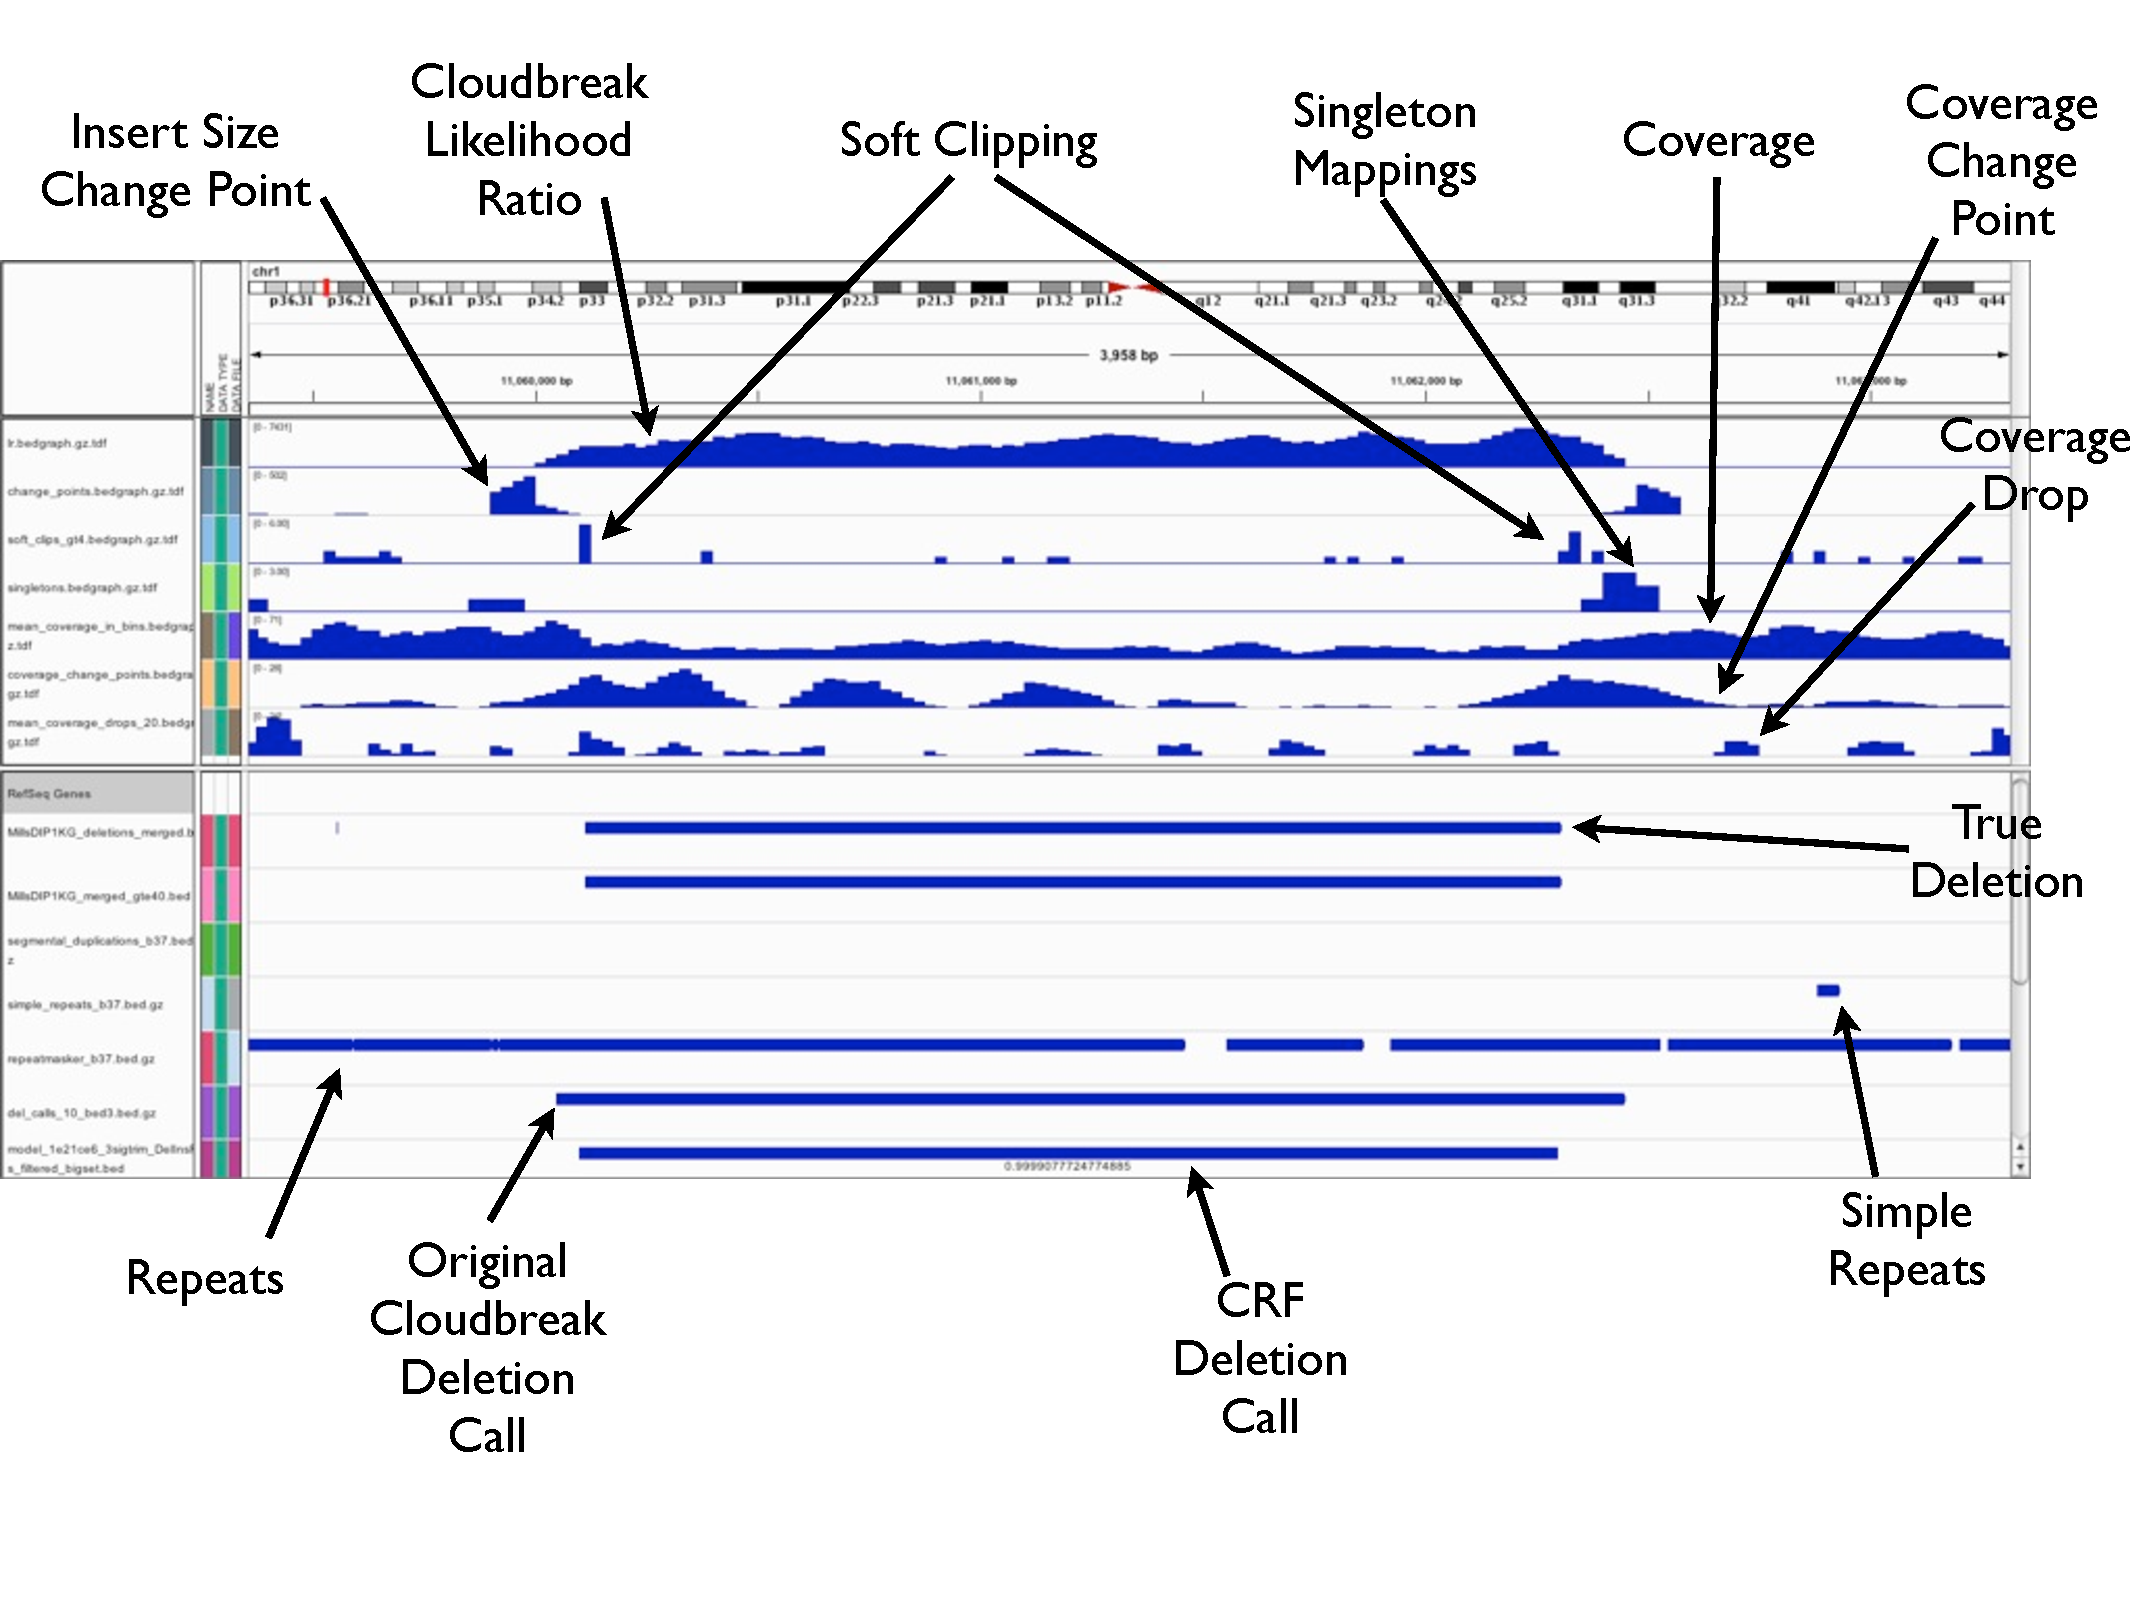
\includegraphics[width=.8\textwidth]{true_example_with_features.pdf}
\caption{An example deletion from the NA18507 data set. The true deletion is shown in track 8. Features shown are in each track are: 1) Likelihood ratio of distribution of insert sizes. 2) Insert size change points. 3) Number of soft clipping events in each window. 4) Number of singleton mappings in each window. 5) Read coverage in each window. 6) Coverage change points. 7) Coverage drops. 11) Simple repeats. 12) Repeats. The original Cloudbreak call is shown in Track 13, and a call made by running inference in the CRF model is shown in Track 14.}
\label{crf_features_example}
\end{figure}

\section{Improving Cloudbreak Calls with CRF Predictions}

\section{Training and Evaluation}
First, I had to decide what data to train and test on. Since we don't have complete annotations of real data sets available, I decided to try training on simulated data. For this, I took my original simulation of chromosome 2 that I did for my Cloudbreak paper and expanded it to a whole genome to try to get more training data, and make the problem a little harder. This simulation includes all of the insertions and deletions annotated for J. Craig Venter's genome. For deletions and insertions with a length over 40bp, there are 5,610 deletions and 6068 insertions. I simulated 30x coverage 100bp paired-end reads with an insert size of 300bp and realigned them to the genome using BWA, as I did for my earlier work. For my test set, I'm using the same data set for individual NA18507, which is 37X coverage with high-quality 100bp paired end reads with an insert size of 300bp. As in my previous work, I then divided both training and test sets into windows of 25bp and computed features for each window.

I also had to choose what data from these sets to feed to the model for training and testing. I ended up creating training windows centered on all of simulated insertion and deletion variants, with flanking regions added on either end. In some runs I've also added all of the Cloudbreak deletion calls made at a very sensitive threshold, so that I could get a lot of false positives into the training set. 

To pick regions to test on, I'm taking the approach of rapidly identifying candidate regions using a fast tool (Cloudbreak in this instance), adding flanking regions to them, and then running the CRF model on those candidate regions to try to label the true variants. This will of course limit the recall of the CRF approach to the recall of the candidate regions I pick but this strategy seemed like a more efficient one than trying to label the entire genome.

\begin{figure}
\centering
\includegraphics[width=\textwidth]{/Users/cwhelan/Documents/svpipeline/figures/NA18507_DELS_ROC_with_CRF.pdf}
\caption{ROC curve showing the accuracy of Cloudbreak calls that have been verified and refined with conditional random field predictions (Cloudbreak-CRF)}
\label{roc_NA18507_with_crf}
\end{figure}

\begin{figure}
\centering
\includegraphics[width=.8\textwidth]{/Users/cwhelan/Documents/svpipeline/figures/breakpointResolutionNA18507_withCRF.pdf}
\caption{Breakpoint resolution of each tool's successful predictions on the NA18507 data set, including Cloudbreak calls which were verified and refined with CRF predictions (Cloudbreak-CRF)}
\label{breakpoint_resolution_NA18507_with_crf}
\end{figure}

\section{Discussion}

As an alternative to CRFs, I will also investigate the use of deep learning techniques such as sequential deep belief networks~\cite{andrew2012:sdbn}, which have been used successfully in sequence processing tasks in speech recognition and other domains.

The outcome of this extension will be: the creation of a training, development, and test set, along with a feature generation scheme and description of the model used; an evaluation of the performance gains that can be achieved, with a comparison to other SV detection approaches; and a discussion of the benefits and drawbacks of using such an approach.


\chapter{Analysis of Evolutionary Breakpoint Features}
\label{chap_breakpoint_analysis}

This chapter describes a data analysis project unrelated to the algorithmic development of Cloudbreak and its extensions, although it is related at the biological level because it deals with genome breakpoints and rearrangements. In addition to being able to locate genomic breakpoints, we also seek to understand the genomic contexts in which they are located to gain insights into their origins. As we discussed in Chapter~\ref{chap_background}, the sequence features of the genome that neighbor structural variations can leave clues about the mechanisms that caused the rearrangements, as in the cases of large homologies that point to the activity of non-allelic homologous recombination (NAHR) or the microhomologies that indicate non-homologous end joining (NEHJ). In this chapter we examine a set of structural variations that have reshaped a genome at the evolutionary timescale: the chromosomal rearrangements of the gibbon genome. We analyze the locations in which the gibbon genome has been rearranged relative to humans and the other apes, first using a smaller set of breakpoint data, and then using the entire gibbon genome reference sequence created by the International Consortium for Sequencing and Annotation of the Gibbon Genome. The associations we discover could help to provide insights into the mechanisms into which the gibbon genome was rearranged. \todo{and perhaps its structure and function} The main contributions of this chapter are 1) the statistical analysis of the enrichment or depletion of certain genomic features in regions of the gibbon genome that have participated in genomic breakpoints, 2) development of an open-source software tool that can harness compute clusters to conduct permutation analysis for statistical enrichment of features in the genome, and 3) a novel, cross-species analysis of the locations of binding sites of the transcription factor CTCF with respect to genome breakpoints in the gibbon family.

\section{Background}

In Chapter~\ref{chap_background}, we described how SVs can occur in the genomes at many different levels, ranging from the rearrangements that occur in populations of cells within a tumor in a single individual, to SVs that are polymorphic within the population of a species, and all the way to the structural differences between the genomes of different species. This last type of rearrangement represents SVs that occurred within a population and then became fixed in that species and were preserved as it evolved and differentiated. 

Rather than identifying them by comparing short-read sequencing data to a reference genome, as has been the focus of the previous chapters, we can detect these evolutionary breakpoints by directly comparing the genomes of species to each other. This can be done biochemically, by mapping the location of individual genes or large fragments of DNA from one species to particular chromosomes in another; this is the case of the BAC analysis we will describe in Section~\ref{gibbon_breakpoint_bac_analysis}. With the advent of whole genome sequences they can be found by conducting sequence alignments (or multiple sequence alignments) of the the reference genomes for the species under study. When species share regions that contain the same genes and other genomic features, in the same order, it is referred to as \emph{shared synteny}. By examining the endpoints of syntenic blocks of the genomes of two species, or \emph{synteny breakpoints}, it is possible to find the breakpoints of the structural variations that rearranged the structure of the two genomes.

Identifying evolutionary breakpoints can give insights into the mechanisms of their formation. It was long thought that chromosomal breakpoints were largely random, such that they are equally likely to occur at any location in the genome~\cite{Ono:1973tr,Nadeau:1984tm}. Higher-resolution analysis, however, revealed that certain regions of the genome are much more likely to give rise to evolutionary breakpoints~\cite{Pevzner:2003ba}, and this result was re-confirmed once whole-genome reference sequences for many species became available~\cite{Murphy:2005hv}. Tantalizingly, Murphy et al. also showed that these reused evolutionary breakpoint regions overlapped significantly with the breakpoints of SVs found in cancer genomes~\cite{Murphy:2005hv}.

This raises the question of whether these regions of the genome have special properties that make them more likely to participate in evolutionary breakpoints. In Chapter~\ref{chap_background}, we described the fact that certain mechanisms for SV formation, in particular NAHR, are a result of having regions with high sequence similarity at different locations in the genome, as the cell's machinery attempts to repair double-stranded breaks in DNA by joining homologous regions together. As one might expect if evolutionary breakpoints were the result of NAHR, a large number of chromosomal rearrangements in mammals, approaching 40\%, are associated with segmental duplications~\cite{Bailey:2004fb,Bailey:2006fn}. Closer examination of breakpoints from a variety of species, including human, chimp, macaque, rat, mouse, pig, cattle, dog, opossum, and chicken, confirmed that they contain more sequence that is not unique relative to the rest of the genome than would be expected by chance, including segmental duplications (SDs) and other low-copy number repeats~\cite{Larkin:2009ij}. However, analysis of evolutionary sequence divergence in these repeats indicates that some of the duplications may have occurred after the rearrangements, casting doubt on the theory that an NAHR-like process is primarily responsible~\cite{Bailey:2004fb}, and indeed the precise mechanisms behind evolutionary breakpoints remain unknown.

Gibbons represent a unique opportunity to study the process of evolutionary genomic rearrangement because of their highly rearranged genomes. In most branches of the evolutionary tree, large genomic rearrangements are rare events, occurring at a rate of approximately two every ten million years~\cite{Wienberg:2004gt}. However, some species appear to have faster or slower rates of rearrangements. For example, the orang-utan genome has very few medium and large scale rearrangements relative to the expected number given its time of evolutionary divergence~\cite{Locke:2011gn}. At the other end of the spectrum, gibbon genomes have 10 to 20 times more rearrangements than would be expected given the rate in other mammals, and in fact the four genera of gibbons have numbers of chromosomes ranging from 28 to 52, suggesting that gibbon genome has been shuffled rapidly since it diverged from the other apes 17 to 18 million years ago~\cite{Misceo:2008kg}.

Given their highly rearranged karyotypes, gibbons represent an excellent model in which to study mechanisms of chromosomal rearrangements. Until recently, however, the whole genome sequence of the gibbon was not available. Therefore, several studies analyzed gibbon genome breakpoints using techniques involving bacterial artificial chromosomes (BACs)~~\cite{Girirajan:2009kw,Carbone:2006jk,Carbone:2009p1012}. BACs are medium sized (150-350kb) fragments of DNA from a sample that are isolated, turned into plasmid bacterial chromosomes, and then amplified in a culture. By probing gibbon BACs with arrays or testing their hybridization to human chromosomes using fluorescent \emph{in situ} hybridization (FISH) experiments, it is possible to isolate BACs which span human-gibbon evolutionary breakpoints. This allows one to locate the breakpoint regions to within several hundred kilobases, and the small size of the BACs relative to the entire genome makes them much easier to sequence, allowing the analysis of sequence features near the breakpoints; or, if sequencing is not possible, to identify the regions orthologous to the breakpoints in the genome of a well characterized genome. Initial studies examined selected BACs from the northern white-cheeked gibbon species \emph{Nomascus leucogenys leucogenys} (NLE) and found a high level of segmental duplications and repetitive sequence at the breakpoints~\cite{Carbone:2006jk,Roberto:2007dt}. Similar results were found in BACs from the white-handed gibbon species \emph{Hylobates lar} (HLE)~\cite{Misceo:2008kg}. A later study increased the scope by examining 24 sequenced NLE BACs that spanned breakpoints, and analyzed gibbon-specific insertions of repeats and segmental duplications at the breakpoints to postulate several possible rearrangement mechanisms~\cite{Girirajan:2009kw}. More recently, Carbone et al.~\cite{Carbone:2009p1012} analyzed 57 NLE BACs and, in addition to segmental duplications, found enrichment for \emph{Alu} repetitive elements. The latter study also found differences in CpG methylation marks on \emph{Alu} elements near the breakpoints, suggesting that there may be an epigenetic process involved in gibbon genomic rearrangements.

\section{Evolutionary Breakpoints in the Gibbon Genome  Identified by BACs}\label{gibbon_breakpoint_bac_analysis}

To determine whether or not the characteristics observed in the breakpoints identified by BACs from NLE and HLE gibbons were generalizable to the entire gibbon family, we conducted an expanded analysis of gibbon breakpoints based on the identification of additional BACs covering breakpoints in the remaining two gibbon genera using samples from the species \emph{Symphalangus syndactylus} (SSY) and \emph{Hoolock leuconedys}. Since each of the gibbon genera has a different karyotype, identifying breakpoints across all four allows for greater insight into the mechanisms and timing of the evolution of the gibbon family. I contributed to this research by analyzing the overlap between breakpoints from all four gibbon genera with genomic features. This work was published in Capozzi et al.~\cite{Capozzi:2012bb}.

\subsection{Methods}

To determine whether there exists an enrichment or depletion for genomic features associated with gibbon chromosomal breakpoints we computed the significance of their overlap using Monte Carlo permutation tests. The purpose of the permutation analysis is to discover the null distribution for the number of overlaps a set of intervals has with a particular feature in the genome. In essence, the test asks: if my intervals were placed in random locations on the genome, what is the probability of seeing the number of overlaps we observed with that features in the actual data? In this case, the intervals whose locations we permute are the gibbon breakpoint regions.

For this test, we identified the human regions that are syntenic to the locations of the breakpoints in gibbons. We then permuted their start coordinates 10,000 times using BEDTools version 2.16.2~\cite{Quinlan:2010km}, while maintaining the chromosomal assignment and length of breakpoint regions. Genomic regions annotated as centromeres and telomeres in the ``Gaps'' track of the hg19 build were excluded from possible random placements of the regions. Locations of the features were held constant. We then compared the actual number of features that overlapped a breakpoint region to the distribution of overlap counts among the randomly permuted regions, and used the quantile of the real observed value in that distribution as an estimate of the P-value of observing a value equal to or greater than the real observation. For events that are rare, it is necessary to consider a large number of permutations or Monte Carlo samples in order to accurately estimate the p-value~\cite{Rubinstein:2007:SMC:1349778}. In order to facilitate conducting many permutations, we created a pipeline for distributing the necessary computation across a compute cluster using the grid management system HTCondor~\cite{condor-practice}.

The analysis was performed on the human hg19 assembly. The features examined were genes, human segmental duplications, and some repeat families (\emph{Alu}, LINE, ERV, and SVA). We also investigated the associations between breakpoint regions and chromatin structure by testing the overlap with open chromatin regions in human embryonic stem cells reported by the ENCODE consortium~\cite{ENCODEProjectConsortium:2011iz}. 

\subsection{Results}

We found a significant enrichment for genes (Bonferroni adjusted P-value = 0.0287), human segmental duplications (P = 0.0366), \emph{Alu} (P < 0.0001), and SVA (P = 0.0008) Figure~\ref{gibbon_bac_permutations} displays the histograms of overlap counts in the random distributions for segmental duplications, \emph{Alu} elements, and SVA elements. We did not find significant enrichment for LINE and ERV repeats, nor for the ENCODE open chromatin regions. SVA elements are not found in gibbons; therefore, their status as significantly enriched in the human syntenic breakpoint regions is surprising. However, SVAs are known to correlate with \emph{Alu} elements due to their preference for G+C rich regions of the genome (Wang et al. 2005). It seems likely that the association between human SVA locations and gibbon breakpoint regions is therefore an indirect one, dependent on the presence of additional genomic features present in both humans and gibbons. 

Systematically shifting the location of breakpoint regions by increments of 10 kb up- and downstream of their actual location, up to a maximum of 1 MB, shows that the locations of the breakpoint regions gives the greatest or close to the greatest number of overlaps with the four significantly overlapping features (genes, segmental duplications, \emph{Alu}, and SVA) in the local genomic neighborhood, also shown in Figure~\ref{gibbon_bac_permutations}.

\begin{figure}
\centering
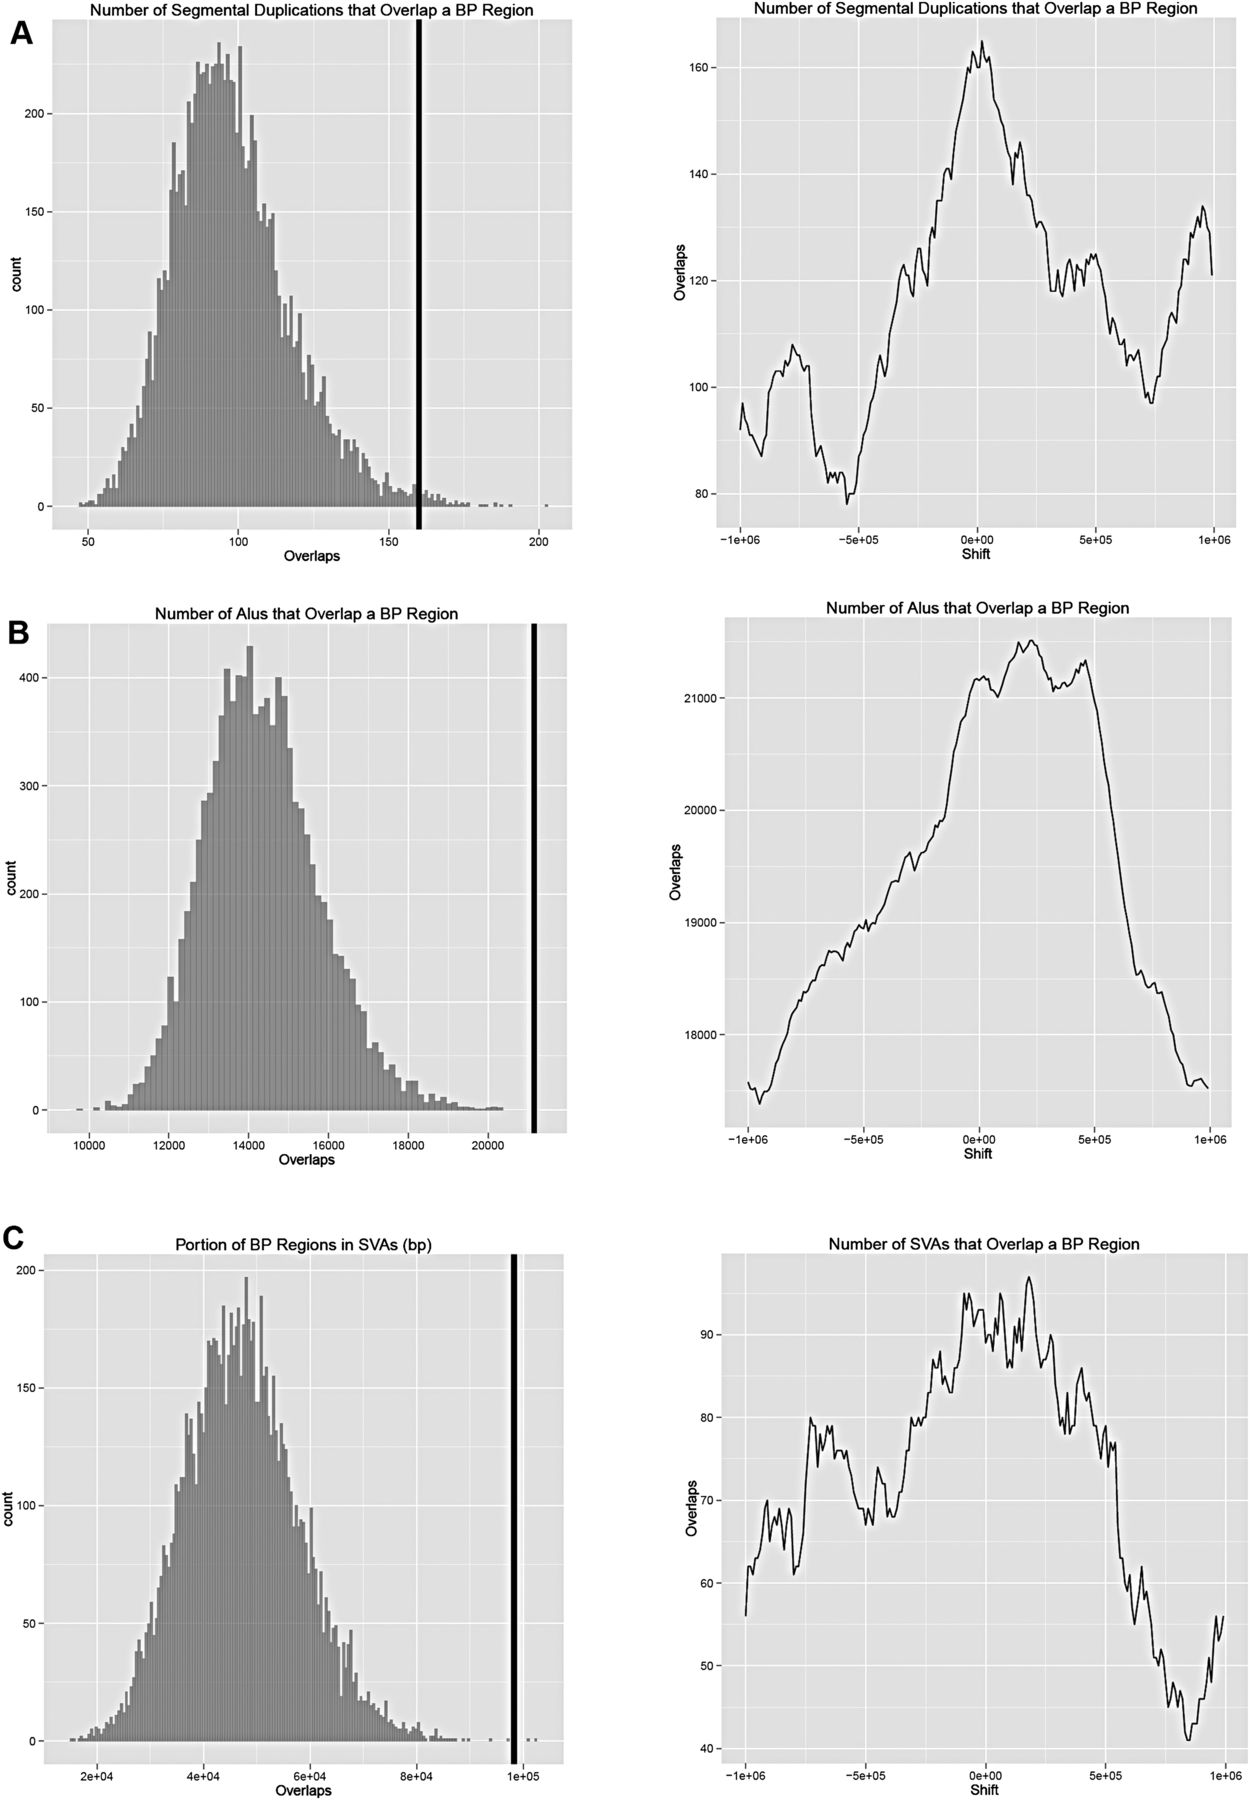
\includegraphics[width=.85\textwidth]{figures/gibbon_bac_permutations.jpg}
\caption{Enrichment of genomic features in regions of the human genome syntenic to gibbon breakpoint regions identified using BACs. Permutation tests were used to assess the overlap between the gibbon breakpoints and genomic features. (A) Segmental duplications; (B) \emph{Alu} elements; and (C) SVA elements. The black vertical line indicates the observed value for the breakpoints identified in the study. In all three cases it is evident that the genomic features have a higher overlap with the breakpoints than one could expect by chance. Figure reproduced from Capozzi et al.~\cite{Capozzi:2012bb}.}
\label{gibbon_bac_permutations}
\end{figure}

\section{Analysis of Breakpoints from the Gibbon Genome Reference Sequence}

While analysis using breakpoints identified with BAC clones has provided useful results, the International Consortium for Sequencing and Annotation of the Gibbon Genome has recently created a draft assembly of the whole gibbon genome for an NLE individual. Comparison of the assembly sequence with the human reference genome has enabled the identification of a complete set of synteny breakpoints between the human and gibbon genomes at single nucleotide resolution. This allows for a much more comprehensive picture of the sequence features surrounding gibbon breakpoints than was previously possible. As a member of the project, I was responsible for the breakpoint analyses described here.

\subsection{Overlap with Genomic Features: Repeats and Genes}

To analyze the enrichment of genomic features in the regions flanking evolutionary breakpoints, we again used a permutation based approach. The number of overlaps between breakpoint flanks and each feature of interest in the assembled genome (the observed overlap count) was again compared to a background distribution estimated by randomly permuting the locations of breakpoint regions 100,000 times. The Nleu1.1 version of the assembly was used for these analyses. To create breakpoint regions, for those breakpoints for which we had single nucleotide resolution we added flanking regions to either side of the breakpoint; for breakpoints that fell within a gibbon-specific repeat element, we chose the flanking regions of the repeat. In each permutation, the location of each breakpoint region was randomly changed, while keeping the length and scaffold assignment of the breakpoint region the same. We then counted the number of overlaps between the randomized breakpoint regions and the feature of interest (the permuted overlap count). Enrichment p-values were computed as the proportion of permuted overlap counts that were more extreme than the observed overlap count. We also visualized the spatial relationship of breakpoint regions to each type of figure by simultaneously shifting the locations of the breakpoint regions up to 1MB in each direction, in increments of 25kb, and counting the proportion of shifted breakpoint regions that overlapped a feature of interest, after discarding regions that were shifted beyond the beginning or end of a scaffold. Permutation testing and shift testing were carried out using custom Python scripts and the BEDtools~\cite{Quinlan:2010km}, pybedtools\cite{Dale:2011cl}, and BEDOPS~\cite{Neph:2012kq} libraries. For this project we enhanced the pipeline and made the code publicly available at \url{https://github.com/cwhelan/permuting-feature-enrichment-test}.

We tested for enrichment in the breakpoint regions of the following features: genes, segmental duplications, and several classes of repetitive elements: \emph{Alu}, L1, LAVA, and LTR. In addition to testing the entire \emph{Alu} family, we also tested the subfamilies \emph{AluS}, \emph{AluJ}, and \emph{AluY} individually. Gene locations were taken from Ensembl build 70. For the segmental duplication analysis, we used the segmental duplications identified by our collaborators in the Eichler laboratory using the WSSD method~\cite{Bailey:2002jp}. \emph{Alu}, L1, and LTR locations were identified using RepeatMasker output. In order to determine the distance from the breakpoints at which enrichments are strongest, we varied the size of the breakpoint flanking regions by adding differently sized intervals; we tested flanking regions of size 100bp, 250bp, 500bp, and 1000bp. We corrected for multiple testing using the FDR under dependency method of Bejamini and Yekutieli~\cite{Benjamini:2001fs}. 

Breakpoint regions are depleted for genes, but enriched for \emph{Alu} elements and segmental duplications. The enrichment for \emph{Alu} becomes particularly strong at distances of 750bp or 1000bp from the breakpoint (Figure~\ref{gibbon_genome_enrich_by_distance}). The enrichment for \emph{Alu} is primarily due to a strong enrichment of the \emph{AluS} subfamily.

\begin{figure}
\centering
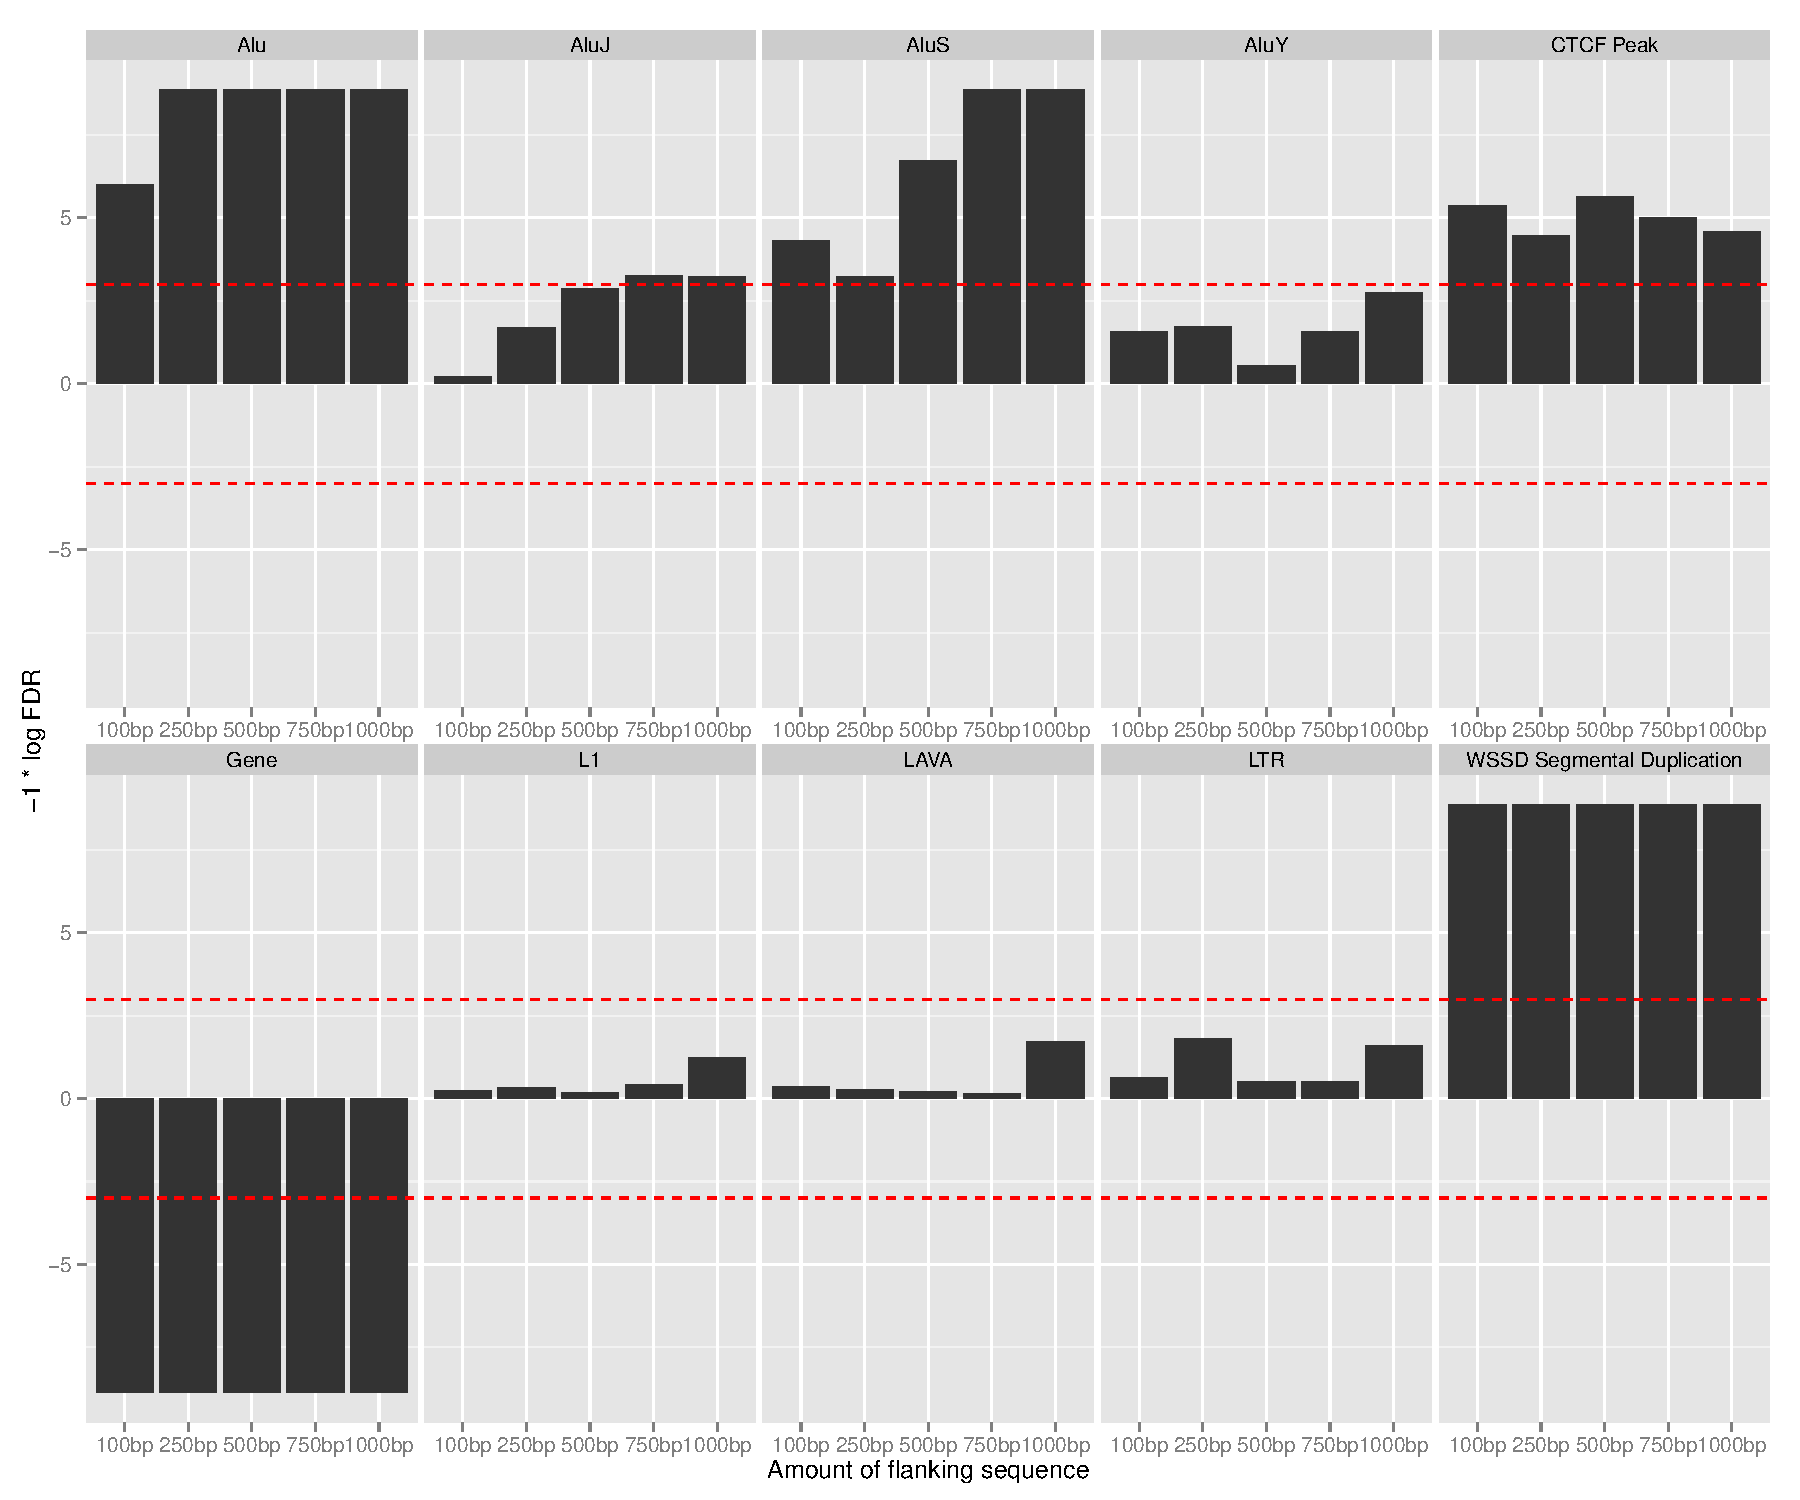
\includegraphics[width=1\textwidth]{figures/regionHitQuantiles.pdf}
\caption{Enrichment or depletion of regions of the gibbon genome for various features, broken down by distance from the breakpoint. Positive y values are the negative log q-values of enrichment for each feature in the regions flanking the breakpoint of the size indicated on the x-axis. Negative y-values represent the q-values of depletion. Q values were calculated using the FDR correction under dependency procedure. The dotted line indicates an FDR threshold of 0.05. Breakpoints are enriched for \emph{Alu} elements, and particularly the \emph{AluS} subfamily, especially at distances of 750bp and 1000bp from the breakpoints. Breakpoints are also enriched for segmental duplications, depleted for genes, and enriched for CTCF binding sites (see Section~\ref{gibbon_ctcf_binding_sites}.)}
\label{gibbon_genome_enrich_by_distance}
\end{figure}

\todo{Even though genes were depleted overall, some of the genes overlapping with breakpoints belong to interesting biological categories \todo{(Table ST5.1 )}.}

In conjunction with our collaborator Larry Wilhelm, in addition to testing the count of overlaps between breakpoint flanking regions and repeats, we also conducted a complementary test that examined the distance of each breakpoint to the nearest repeat of a given class. For this test we used only the 44 breakpoints for which we had single nucleotide breakpoint resolution, with no Gibbon-specific repeats directly intersecting the breakpoint. We compared these breakpoint locations to 10,000 randomly selected regions in the nomLeu2 genome. For each random location, we determined the distance to the nearest repeat. We compared the distribution of distances to a repeat from the breakpoints to the distribution of distances to a repeat from the randomly selected positions using a Kolmogorov-Smirnov test. We examined the distance to any repeat, as well as those for \emph{Alu}, LINE, and LTR elements, and finally the \emph{AluJ}, \emph{AluS}, and \emph{AluY} subfamilies. After FDR correction for multiple hypothesis testing, the distance test showed similar results to the overlap test described above, with significant results for the \emph{Alu} family as a whole, and for the \emph{AluJ} and \emph{AluS} subfamilies, indicating that the breakpoints tend to be closer to those repeats than random locations in the genome.

We also conducted a shift analysis similar to that displayed in Figure~\ref{gibbon_bac_permutations}. Breakpoint regions were simultaneously shifted in increments of 25kb, up to a maximum of 1MB in each direction, and the proportion of breakpoint regions that overlap a feature of interest is reported. Shifts show that breakpoints are centered on regions that are depleted in genes but close to regions that contain genes, while the opposite is true for segmental duplications. \emph{Alu} elements are more evenly spread across the shift regions (Figure~\ref{gibbon_genome_feature_shifts}).

\begin{figure}
\centering
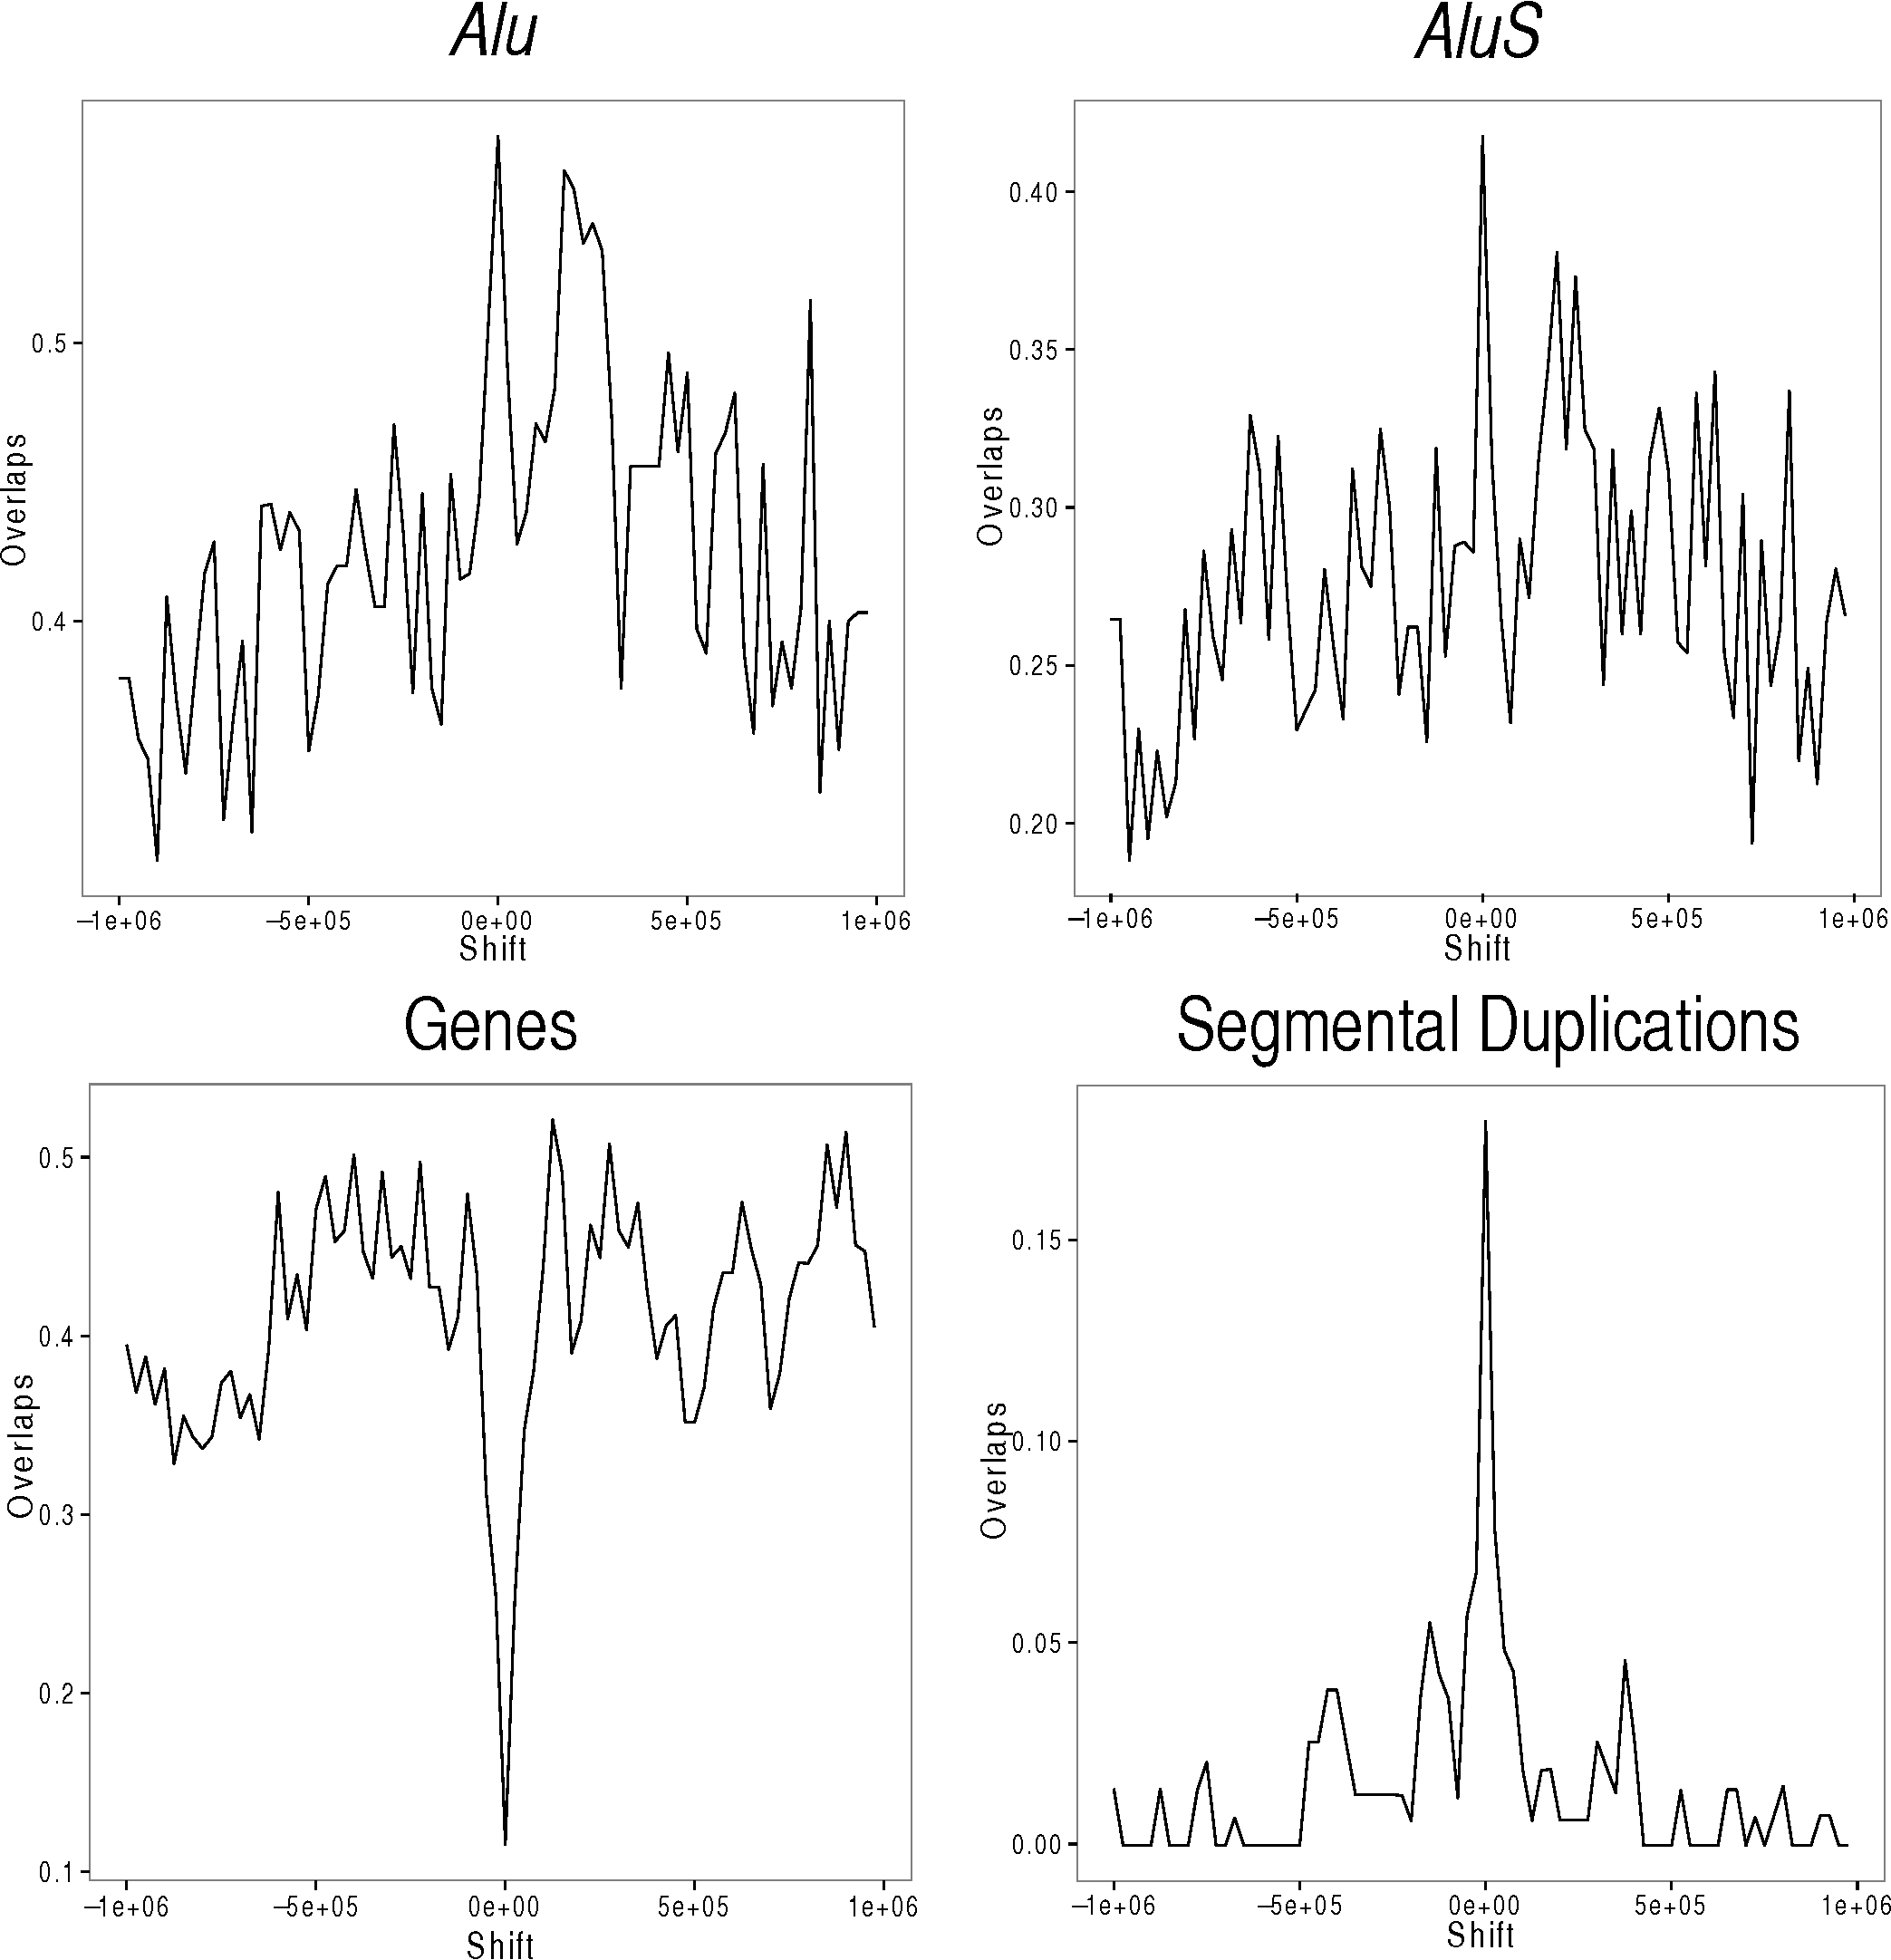
\includegraphics[height=.75\textheight]{figures/gibbon_genome_feature_shifts.pdf}
\caption{The proportion of breakpoint flanking intervals (defined as the 1000bp intervals flanking exact breakpoint locations or gibbon-specific repeats located at the breakpoints) which overlap with a feature of interest, when the flanking intervals are shifted left or right from their actual locations. Breakpoints are located in locations enriched in \emph{Alu} (especially \emph{AluS}) and segmental duplications relative to their genomic neighborhoods, but which are depleted for genes relative to their genomic neighborhoods.}
\label{gibbon_genome_feature_shifts}
\end{figure}

\subsection{Overlap with CTCF Binding Sites}\label{gibbon_ctcf_binding_sites}

Using the gibbon genome reference, we conducted another set of analyses to determine the relationship of gibbon genome breakpoints with binding sites of the evolutionarily conserved binding factor CTCF. CTCF is a transcription factor with many functions, including the ability to separate regulatory domains in the genome from one another~\cite{Phillips:2009fr}. CTCF has also recently been shown to be associated with the three-dimensional structure of DNA and chromatin in the cell~\cite{Dixon:2012gc}, and therefore may have important associations with genomic DNA breakpoints and structural variations. We examined CTCF in the gibbon through the analysis of chromatin immunoprecipitation followed by sequencing (ChIP-seq) data~\cite{Park:2009gl}. Briefly, in ChIP-seq DNA from a sample is cross-linked \emph{in vivo} and then fragmented, so that proteins (in particular transcription factors) remain bound to the fragments of DNA that contain their binding sites. After selecting only those fragments with a bound protein of interest using immunoprecipitation, the DNA is then sequenced. Mapping the reads back to the genome reference sequence creates ``peaks'' of coverage along the genome that indicate the location of transcription factor binding sites. In this analysis we identified a set of CTCF binding sites using gibbon ChIP-seq data, and conducted a comparative analysis using CTCF peaks from other primate species to separate CTCF peaks shared with a common ancestor from those that are unique to gibbons.

\subsubsection{ChIP-seq for CTCF}

CTCF ChIP-seq assays were performed by our collaborators in the laboratories of Duncan Odom and Paul Flicek according to the protocols described in Schmidt et al.~\cite{Schmidt:2012dt} on eight EBV-transformed gibbon lymphoblastoid cell lines. In brief, CTCF-bound DNA was immunoprecipitated using an Anti-CTCF rabbit polyclonal antibody (07-729, Millipore). End-repair was performed on immunoprecipitated and input DNA prior to A-tailing and ligation to single-end Illumina sequencing adapters. DNA was amplified using Illumina primers 1.1 and 2.1 in an 18-cycle PCR reaction. Gel electrophoresis was used to select 200-300 bp DNA fragments. DNA libraries were sequenced using 36 bp reads on an Illumina Genome Analyser II according to the manufacturer's instructions.

\subsubsection{Peak Calling from CTCF ChIP-seq Data}

We aligned reads to the nomLeu2 reference using BWA (version 0.62)~\cite{Li:2009p836} with default parameters, and removed non-uniquely mapping reads. We then called peaks using CCAT~\cite{Xu:2010fu}, with parameters fragmentSize 100, slidingWindowSize 150, movingStep 10, isStrandSensitiveMode 1, minCount 10, minScore 4.0, and bootstrapPass 50. We then combined the peaks called across the different individuals and chose the following set for further analysis: any peak called in an individual individual by CCAT with an FDR of less than 0.05, as well as any peak that was called in more than one individual with an FDR of less than 0.1. \todo{(Table ST5.2)}

\subsubsection{Determination of Gibbon-specific and Shared CTCF Binding Sites}

We classified Gibbon peaks as shared or gibbon-specific by comparing them to a set of CTCF peaks called on human, macaque, and orangutan individuals~\cite{Schwalie:2014}. This work was carried out in conjunction with our collaborators Javier Herrero and Larry Wilhelm. First, orthologous locations of gibbon CTCF peaks in other primate species were determined using a local installation of the EnsemblCompara multi-species alignment database~\cite{ensembl_compara,Vilella:2009ju}. This database contains alignments of the references for human (GRCh37), chimp (CHIMP2.1.4), gorilla (gorGor3.1), orangutan (PPYG2), rhesus macaque (MMUL\_1), and gibbon (Nleu1.1). Gibbon CTCF peaks for which no multi-species alignment were present, or where the nucleotide alignment identity to human and macaque was less than 70\%, were excluded from analysis. We then created a non-redundant list of non-gibbon CTCF peaks by converting the human, orangutan and macaque peaks to gibbon coordinates using the Compara database and removing redundant entries. Shared and gibbon-specific CTCF peaks were then identified as those gibbon CTCF peaks that did or did not intersect a peak in the non-redundant list of non-gibbon CTCF peaks.

\subsubsection{Analysis of Enrichment for CTCF Binding Sites in Gibbon Genome Breakpoints}

We identified 52,685 gibbon CTCF binding sites from the eight individuals. We found that 12 of the 1kb regions flanking breakpoints overlap with CTCF binding sites (see Figure~\ref{example_ctcf_breakpoint} for an example). Using the same permutation analysis described above, this overlap has an enrichment p-value of 0.0009. This effect was even stronger when we expanded the breakpoint flanking regions to 25kb, as 95 expanded flanking regions overlap CTCF peaks for an enrichment p-value <0.0001\todo{(Extended data figure 2)}.

\begin{sidewaysfigure}
\centering
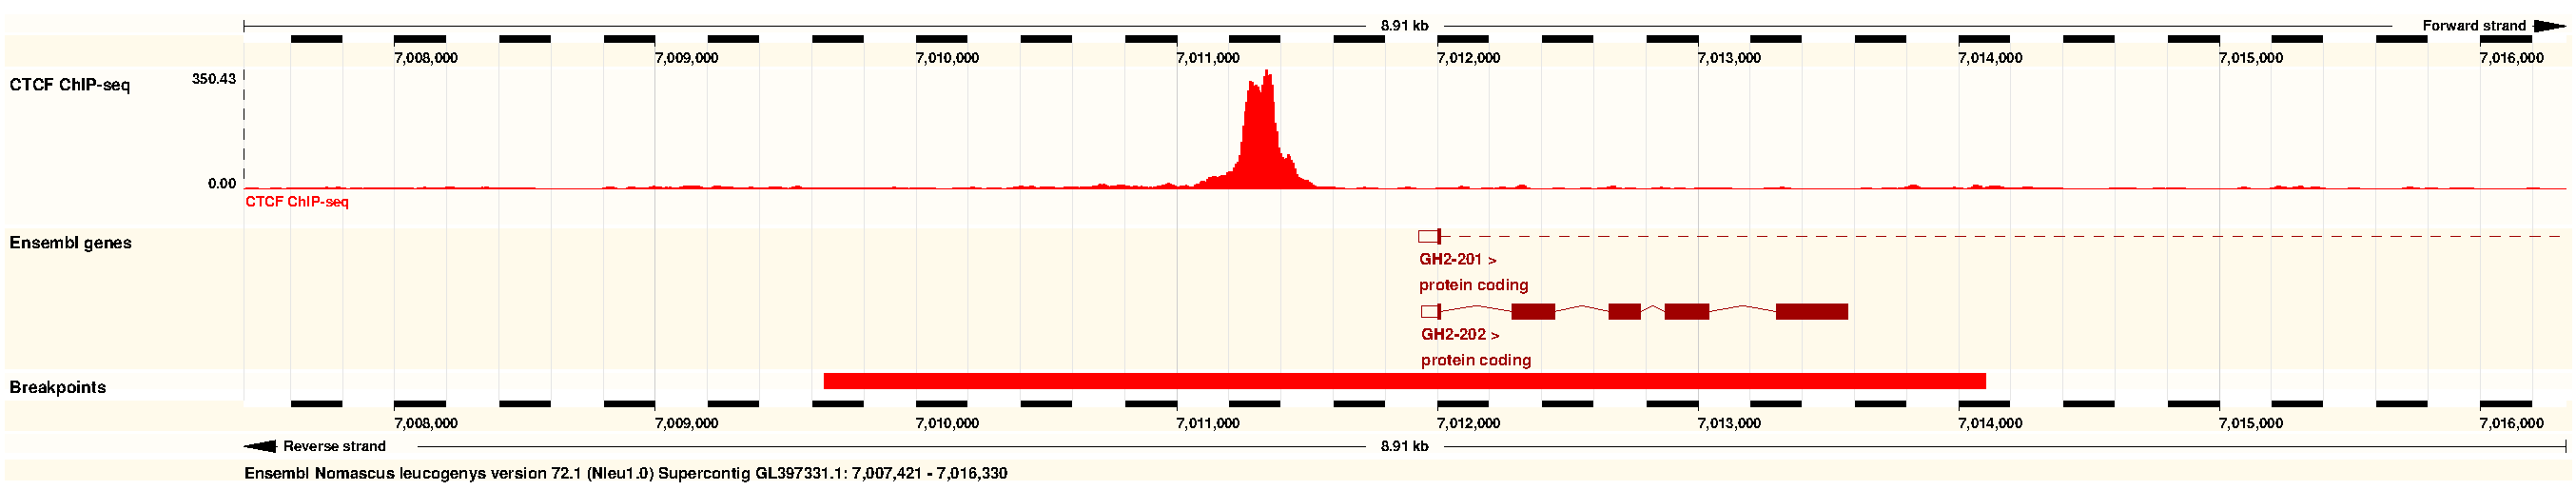
\includegraphics[width=1\textwidth]{figures/merged_CTCF_GL397331.pdf}
\caption{An example of CTCF binding sites in a breakpoint region. The track labeled ``CTCF ChIP-seq'' shows merged read coverage depth from the eight gibbon CTCF ChIP-seq samples, clearly showing a peak representing a CTCF binding site. The ``Breakpoints'' track shows the location of a gibbon breakpoint region. This breakpoint also contains a protein-coding gene, GH2-202.}
\label{example_ctcf_breakpoint}
\end{sidewaysfigure}

We then tested whether the CTCF peaks causing the enrichment in breakpoint regions are specific to gibbons. Using the CTCF ChIP-seq data from other species described above, we classified CTCF binding sites as unique to gibbons (11,449 sites) or shared with a primate ancestor (41,236 sites). We found that the gibbon breakpoint regions are heavily enriched for CTCF binding sites shared with a primate ancestor (enrichment p-value = 0.0006) but are not significantly enriched for gibbon-specific CTCF binding sites. Again, the enrichment is stronger in the 25kb expanded breakpoint regions (enrichment p-value <0.0001) for shared binding sites, but not for gibbon-specific binding sites. This suggests that the formation or selection of gibbon genome rearrangements was associated with ancestral CTCF binding sites.

\todo{I am also helping to analyze the breakpoints from a set of over forty mesenchymal tumor samples in which genomic rearrangements have created ring-shaped chromosomes. The breakpoints that cause these chromosomal rearrangements cluster into several frequently broken areas. I am currently working on analyzing these breakpoint regions using my permutation analysis pipeline in order to determine genomic features that may be significantly associated with these breakpoints, including repeat elements, open chromatin sites and other data from ENCODE, and binding motifs for enzymes known to be involved with breakpoint formation.}

\section{Discussion}

In our work examining breakpoints that included data from HLE and SSY gibbons, we extended previous analyses that had only considered data from NLE. This confirmed that the associations between breakpoints and segmental duplications, genes, and repetitive elements of the \emph{Alu} family previously observed in NLE extended to breakpoints in other genera of the gibbon family. Extending this analysis to the other genera should assist the study of gibbon chromosome evolution, especially when used in conjunction with the release of the gibbon genome reference, which is based on data from an NLE individual.

In Capozzi et al.\cite{Capozzi:2012bb}, we were surprised to find an association between breakpoints and genes given that most genome breaks will have deleterious effects if they occur in coding or regulatory sequence. However, we noted that those results were based on analyzing the features of the human genome reference that are orthologous to the gibbon breakpoint regions, and that the result might change when the full gibbon genome sequence was available to be tested. Indeed, that proved to be the case, as the depletion for genes in the breakpoints from the gibbon reference data shows. This could be an interesting finding in itself, as regions of segmental duplication, which are enriched according to both data sets, are progenitors of novel genes and gene families~\cite{Bailey:2006fn}, possibly providing an explanation for the presence of genes in the orthologous human breakpoint regions.

Our discovery that gibbon genome breakpoints are enriched for CTCF binding sites indicates that there is a connection between regions with similar regulatory environments and the genome rearrangements preserved in the gibbon family, and the fact that breakpoints are only enriched for CTCF binding sites shared with gibbon's common ancestors suggests that the heavy rearrangement of the gibbon genome may have had to respect existing regulatory domains; breakages in other locations may have been too deleterious to survival to be preserved through evolution. In addition, the interaction between genomic structural variation and the three-dimensional structure of DNA in the cell is just beginning to be explored~\cite{Dixon:2012gc}, but it is interesting to hypothesize that locations where the three-dimensional conformation of chromatin in the cell change, as represented by CTCF binding sites, might be vulnerable to genomic breakage under certain circumstances that may have been present in the gibbon's evolutionary past.

\chapter{Future Work}\label{chap_future_work}

In this thesis we have demonstrated that distributed computing, in the form of Hadoop and MapReduce, can be applied to the SV detection problem, enabling highly accurate algorithms with very fast runtimes. In addition, we showed that the use of discriminative sequence labeling techniques, in the form of conditional random fields, can be used to integrate many different signals of SVs and by doing so can improve Cloudbreak's results. We hope that the work presented in this thesis is not only useful in itself but is extensible enough to contribute to additional innovations in the detection of structural variations.

\section{Cloudbreak}

There are many possible extensions that could be made to enhance Cloudbreak's effectiveness as a general SV analysis tool for high-throughput sequencing data. These include:

\begin{itemize}
 \item \emph{Support the detection of additional SV types such as longer deletions, inversions, and translocations}. These would be useful and necessary additions to a complete variant detection pipeline. We hope that the abstract formulation of our MapReduce framework in Chapter~\ref{chap_framework} will create a base from which to extend Cloudbreak's capabilities and implement many additional SV detection algorithms in the future. For example, detection of small to medium-sized inversions could be realized by adding the orientation of mapped read pairs as an additional component of the mixtures used in Cloudbreak's feature generation function. One difficulty in this effort will be the relative lack of validated SVs that are not deletions and inversion to develop and test against, but as large scale projects such as the 1000 Genomes continue to generate data this concern should be mitigated.
 \item \emph{Extend Cloudbreak's GMM-based feature generation function to relax the assumption of a diploid genome sample}. Currently Cloudbreak forces a GMM with two components. This assumption would not apply for some sequencing projects, especially in cancer-related research. In a heterogeneous tumor sample, for example, there may be multiple tumor sub-clones, as well as normal DNA, in the sequenced sample, and each set of input DNA might have different genotypes. With additional modeling of these mixtures, it might be possible for Cloudbreak not only to detect different variants in a sample but also to estimate their relative abundances, something that would be useful for tracking tumor clone evolution.
 \item \emph{Add a local assembly step to increase breakpoint resolution and validate SV candidates.} Cloudbreak's breakpoint resolution is lower than that of many other RP algorithms. Although we improved that result in Chapter~\ref{chap_crf}, we could not obtain single nucleotide resolution, because our features were defined in terms of fixed-size genomic windows. As we mentioned in Chapter~\ref{chap_related_work}, one approach to improving breakpoint resolution, and providing additional validation of predicted results, is to attempt to conduct a \emph{de novo} assembly of the reads that mapped near the breakpoints as well as their paired sequences. If effectively implemented, this would be a very useful addition to any SV detection algorithm. Theoretically, each breakpoint could be assembled simultaneously in reduce tasks in an additional MapReduce job. This would greatly increase the confidence and utility of Cloudbreak's predictions.
 \item \emph{Support the simultaneous analysis of multiple samples and libraries.} Approaches such as Genome STRiP~\cite{Handsaker:2011ki} have demonstrated that they can achieve higher accuracy than single-sample SV detection algorithms by simultaneously considering many samples at once. Even if a variant is only supported by a very low number of reads in each individual sample, by pooling data from multiple samples the presence of a variant can become clear. Additional modeling in Cloudbreak of multiple samples, each with its own insert size distribution, might provide a similar increase in power. Alternatively, data could be pooled in Cloudbreak and the resulting predictions could be used as features in our discriminative machine learning models.
 \item \emph{Adopt emerging standardized Hadoop libraries and file formats.} As more effort is put into developing Hadoop-based sequencing analysis applications, it will become increasingly important that these applications use consistent APIs and data formats so that they can be composed into large pipelines. Once they contain the requisite features, refactoring Cloudbreak to use libraries such as Hadoop-BAM~\cite{Niemenmaa:2012hu} would be a step in that direction.
\end{itemize}

\section{SV Detection with Discriminative Machine Learning}

We believe that the application of CRFs to SV detection we described in Chapter~\ref{chap_crf} is very promising and could be extended in many directions:

\begin{itemize}
\item \emph{Construction of improved training data sets.} The most obvious limiting factor for this project was the training and test data used. Training on simulated data ignores many potential sources of noise as well as possible signals that could be used to detect SVs. Training on real data sets, such as those that are being generated for the 1000 Genomes project, would allow much greater potential for learning.
\item \emph{Using additional or different sets of labels.} In some sequence labeling tasks, it can improve performance to model the start and end of variants with separate labels, or to use different types of labels for flanking sequence. It would be useful to test different labeling schemes to determine the optimal one for this task. In addition, the authors of forestSV~\cite{Michaelson:2012fj} demonstrated some utility in directly labeling regions known to cause false positives for other algorithms in training their classifier; this might be useful in our model as well.
\item \emph{Add additional features to the model.} There are many possible additional features that could be used in our model. One example would be possible SNVs near the breakpoint locations, indicated by mismatches between the reads and the reference. There are also many other possible genome annotations or sources of prior knowledge that could be used as features, including the locations of previously identified variants in other samples. 
\item \emph{Learning for additional variant types.} As mentioned above, it would be useful to train our model to detect additional variant types by expanding the label set and set of features used
\item \emph{Alternative learning methods.} Recently, many advances have been made in machine learning for sequencing labeling tasks through the use of deep learning using artificial neural networks. With additional data to train on, it may be possible to apply these techniques to the SV detection problem.
\todo{\item Integrate generation of training and testing data seamlessly into the Cloudbreak workflow.}
\end{itemize}

\section{Gibbon Genome Breakpoint Analysis}

The identification of enrichment of genomic features at the location of gibbon-human synteny breakpoints can be used as background for further research into the evolutionary history of gibbons, with an ultimate goal of understanding the processes that caused them:

\begin{itemize}
\item \emph{Analysis of epigenetic marks associated with breakpoints.} The Carbone lab has been investigating epigenetic signatures near genomic breakpoints, and has found distinct patterns of DNA methylation in breakpoint-associated transposable elements~\cite{Lazar:2014}. DNA methylation may have a role in the formation or conservation of rearranged genomes. Further analysis may reveal new mechanisms of gibbon genome rearrangement.
\item \emph{Exploration of association of large DNA structures and domains with breakpoints.} The association of CTCF binding sites with gibbon breakpoints suggests a possible relationship between rearrangement sites and the three dimensional structure of DNA. Alternatively, CTCF's role as separator of regulatory domains may have rendered genome rearrangements that did not respect those boundaries unviable, causing only those present in today's gibbons to be preserved. Additional analysis of other types of data may allow us to gain insight into these questions.
\end{itemize}


% The library likes numbers rather than the `alpha' style.
\bibliographystyle{acm}
% Single space the bibliography to save space.
\begin{singlespace}
\bibliography{thesis}
\end{singlespace}
%\printbibliography

% The appendices are optional, but they must follow the references.
%\appendix

% This section (the final one) contains a biographical note.
%
%\vita
%This section contains a biographical note.
%The following information (in essay form) should be contained in this section:
%place of birth; date of birth; schools attended; degrees awarded; areas of
%special interest; relevant profession experience; awards and honors; list
%of publications.

\end{document}
